\documentclass[a4paper,10pt]{book}
\usepackage[utf8]{inputenc}
\usepackage{graphicx}
\usepackage[hidelinks]{hyperref}
\usepackage{amssymb}
\usepackage{amsmath}
\usepackage{mathtools}
\usepackage{framed}
\usepackage{mdframed}

\usepackage{helvet}
\renewcommand{\familydefault}{\sfdefault}

\usepackage[margin=1in]{geometry}

\setcounter{secnumdepth}{3}
\setcounter{tocdepth}{4}

\title{{\LARGE\bf{RobotSDK 4.0 : A Complete Top-down Modular Software Development Framework}} \\ {\Large[Quick Manual]}}
\author{HMW-Alexander}
\date{2015-04-18}

\begin{document}

\maketitle
\tableofcontents

\chapter{Introduction}

After two weeks of hard programming with many accumulated new ideas and important feedbacks, a powerful RobotSDK 4.0 is coming.
It has indeed realized a complete top-down software development framework compared with its predecessors, but still follows their principle of abstract graph model and modular software development.

\section{New Features of RobotSDK 4.0}

\subsection{Robot-X}

For RobotSDK 2.1, 2.2 and 3.0, users need to program a high level application to realize a conceptual graph-model, in which functional modules could embed. Although, RobotSDK 3.0 provides a set of simplified functions to draw such graph-model, users are still trapped in the problems like misspelling of node name, frustrating complex network and confusion of node types.

Now, in RobotSDK 4.0, instead of programming annoying high level applications, users only need to draw it on Robot-X without considering different node types (Fig.\ref{fig:robotx}). And then, users can freely embed required functional modules via shared library and fully control all nodes in it. Therefore, in RobotSDK 4.0, for common development, additional high level programming is not needed.

Meanwhile, Robot-X provides a convenient Config Panel UI (Fig.\ref{fig:configvalue}) to modify configuration values in XML file for each node. With this tool, users need not to manually modify confused XML config file.

\begin{figure}
 \centering
 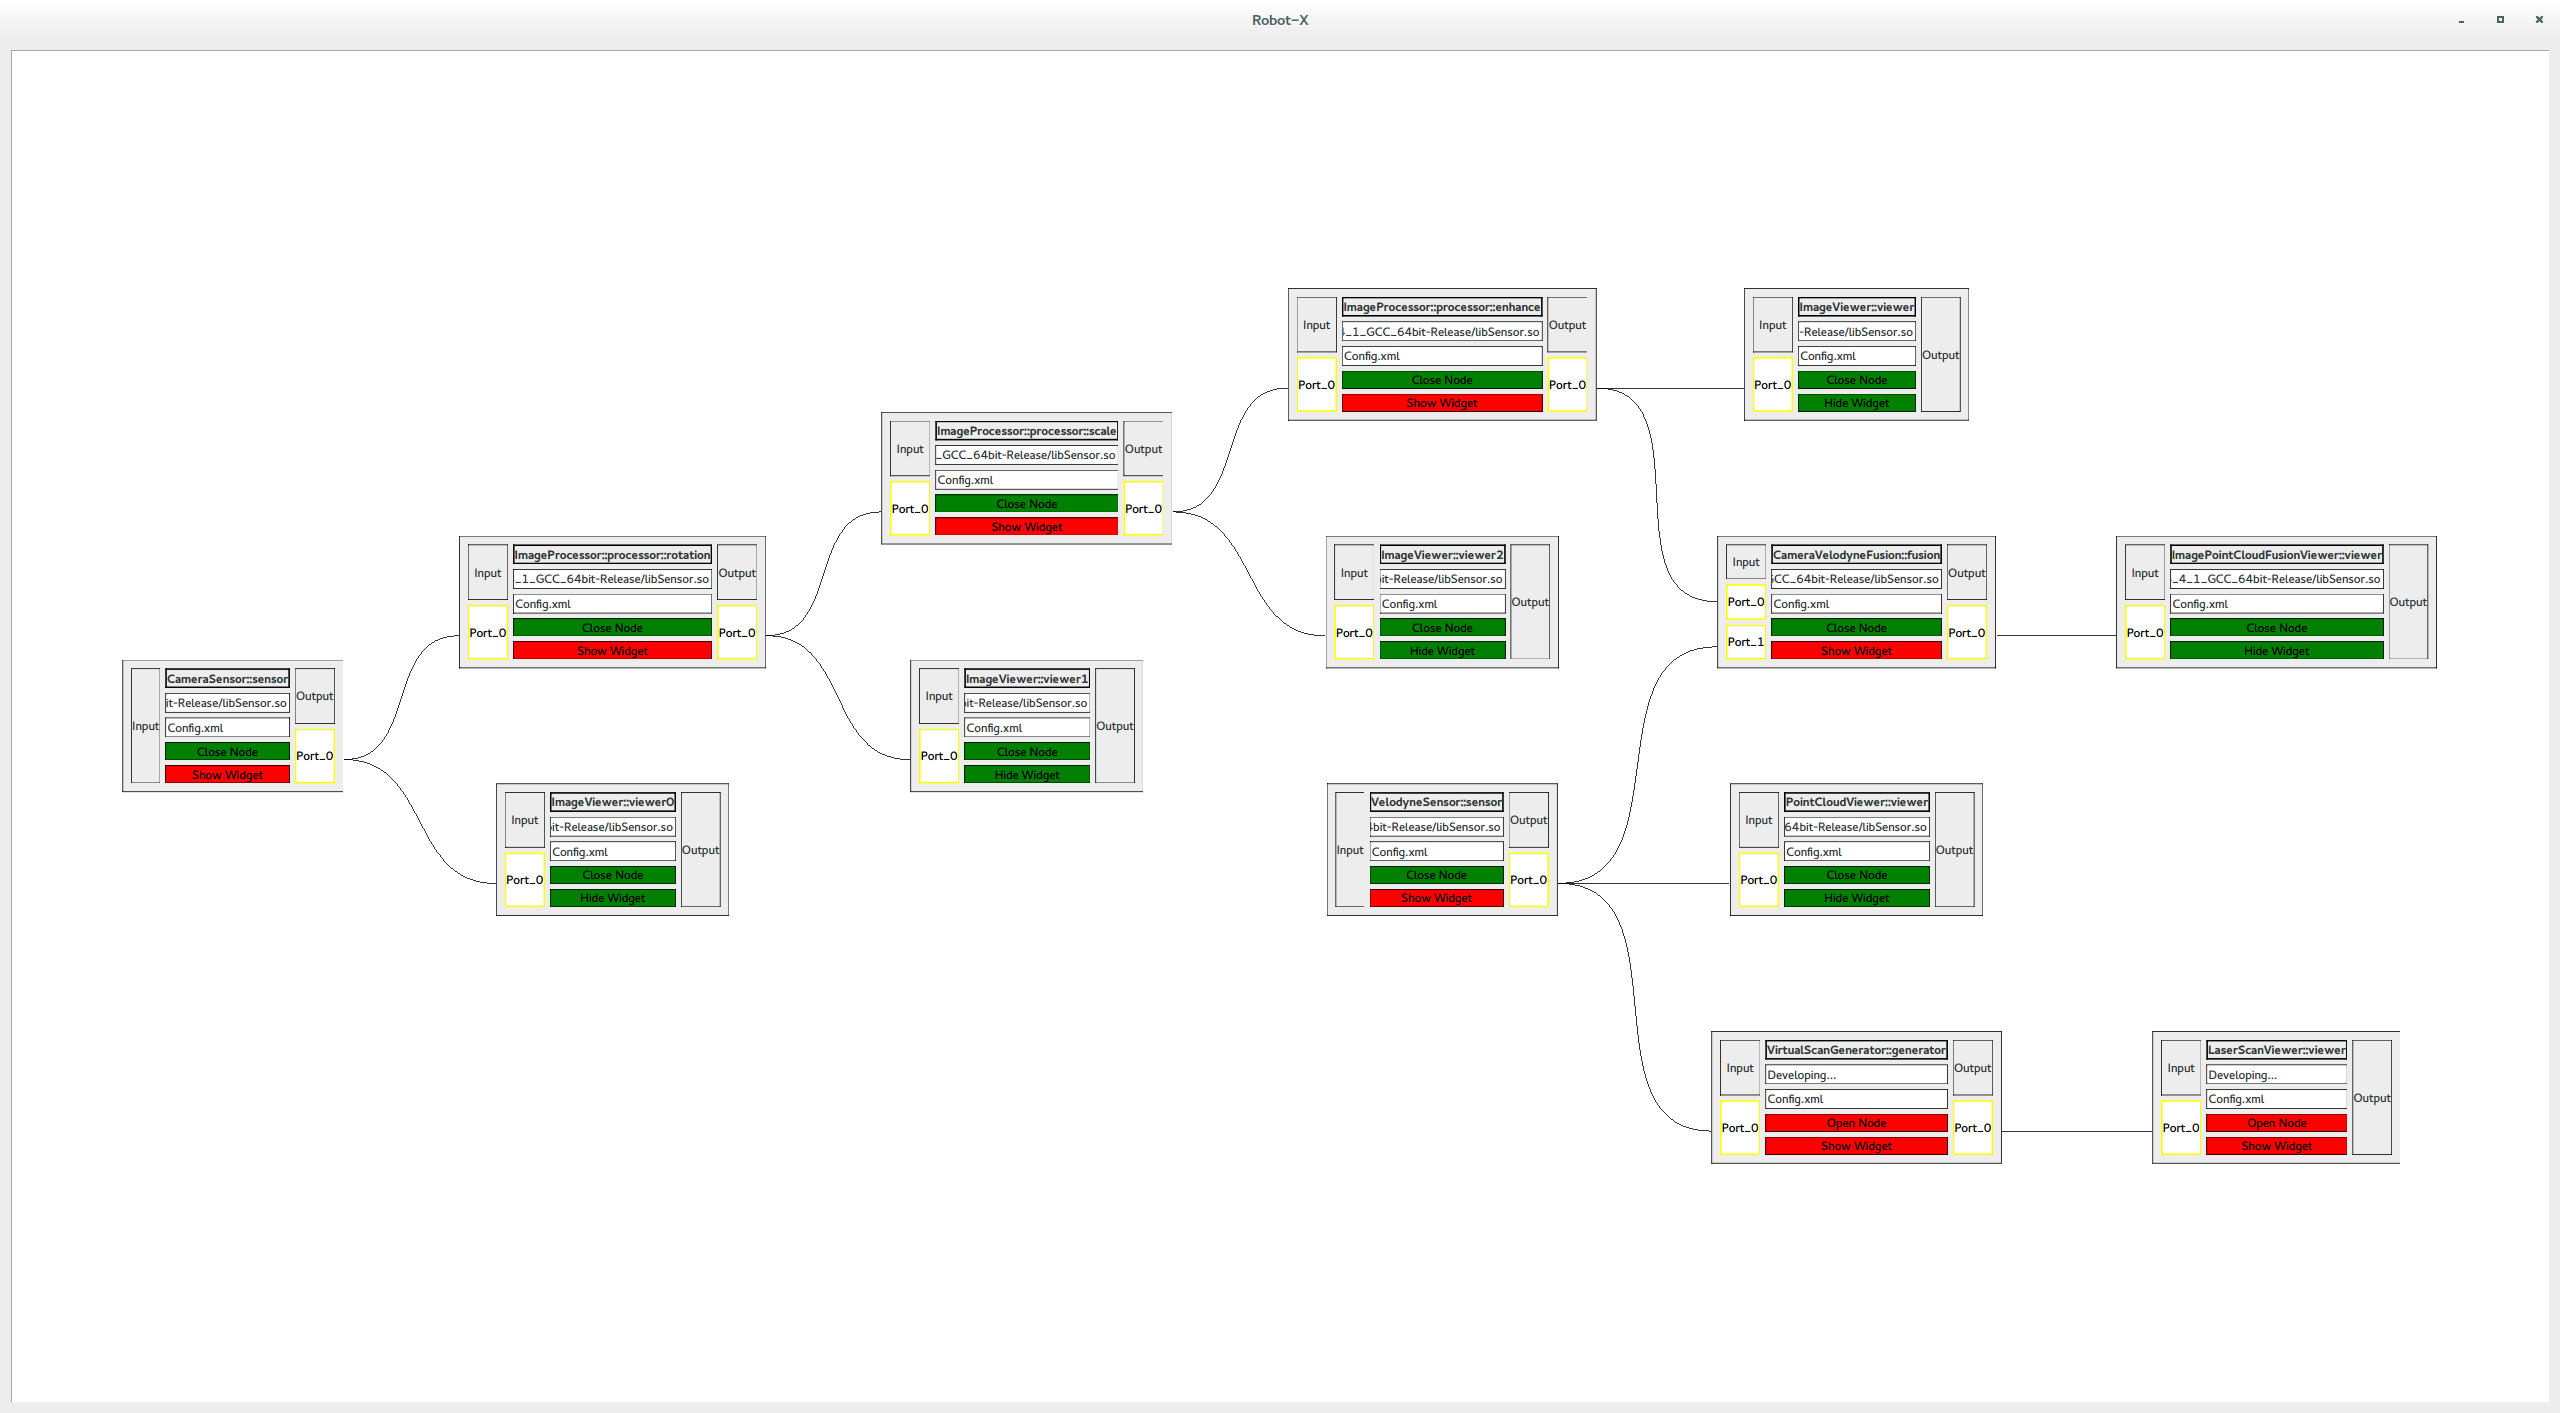
\includegraphics[width=0.8\textwidth]{img/Robot-X.png}
 \caption{Robot-X and the Conceptual Graph-Model}
 \label{fig:robotx}
\end{figure}

\begin{figure}
 \centering
 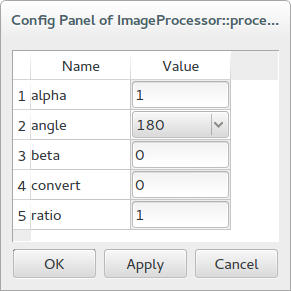
\includegraphics[width=0.2\textwidth]{img/configvalue.png}
 \caption{Config Panel UI to modify configurations values of ImageProcessor node}
 \label{fig:configvalue}
\end{figure}

\subsection{Simple and Free Module Development}

From RobotSDK 2.2, assistant tools were created to automatically generate interface source codes for module development. However, the auto-generated source codes are so long and complex that developers could not easily handle them. About 40\% error feedbacks are related to such sick source codes. Another bad thing is that the auto-generated source codes limited developers to their constant frame and even for experienced developers, it is not free to program modules as they want.

For RobotSDK 4.0, thanks to C++11 techniques, the module development becomes simple and free. The auto-generated interface source codes become very short and for each module, the number of generated files shrinks from 6 to 2 (1 header and 1 source). Moreover, a set of intuitive syntax is introduced to simplify programming. For functions development, there is no constant framework. Just like C programming, it only needs a entry function, which is also named as "main", therefore, developers can freely program module in C style.

\subsection{Kernel Update}

Up to now, there are about 50\% bug feedbacks are related to Kernel and there are 4 critical bugs related to design defects of RobotSDK 3.0:
\begin{enumerate}
 \item Data stream is not stable: caused by unbalanced producer-consumer model.
 \item Simulator is not accurate: caused by mixture of intra-thread and inter-thread communication.
 \item Timestamp of received data is not accurate: same with 2.
 \item High-speed data stream overwhelms others with low-speed for node while using Edge Monitor: same with 2.
\end{enumerate}

In RobotSDK 4.0, the construction, maintenance and destruction of data stream are redesigned after learning related Qt source codes.

Each node, if it has input, output and some intrinsic triggers, it will have 4 independent threads: Main thread, InputPorts thread, OutputPorts thread and QObjectPool thread. Unlike RobotSDK 3.0, these threads will not be closed until the node is destroyed (not closed, see abstract node state machine in Fig.\ref{fig:nodestate}). Therefore, even the node is closed, the independent input ports could still receive data in its InputPorts thread and also send the packed data (if and only if the port buffer fulfills user's requirement) to the Main thread. Then, for the node thread, it uses a EventFilter technique provided by Qt to filter out packed data when the node is closed. This guarantees the balance of producer-consumer model, as well as no deadlock while closing node.

\begin{figure}
 \centering
 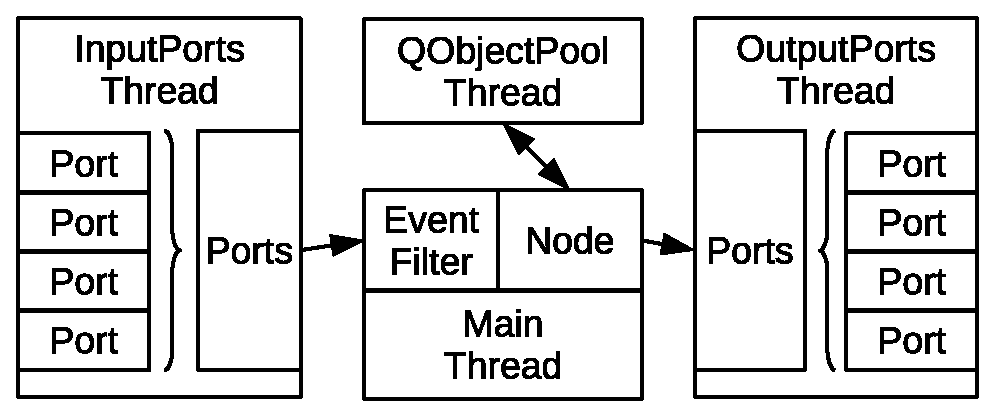
\includegraphics[width=0.4\textwidth]{img/threads.eps}~~
 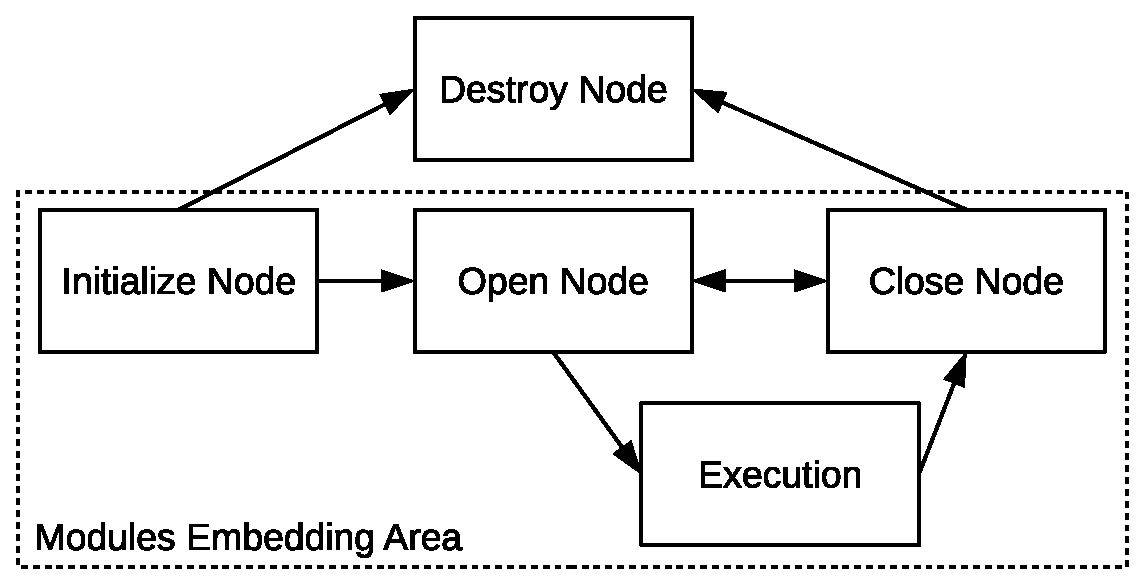
\includegraphics[width=0.4\textwidth]{img/nodestate.eps}
 \caption{Threads of a node and abstract node state machine}
 \label{fig:nodestate}
\end{figure}

The mixture of intra-thread and inter-thread communication is the most significant design defect of RobotSDK 3.0. The default intra-thread communication between signal and slot is direct call and the inter-thread communication between them is based on event-loop. The direct call would block event-loop and event-loop itself means lag existence for high frequency communication. I will explain the problems with some examples below.

Take Simulator in RobotSDK 3.0 for example, it takes a QTimer in the abstract node to trigger itself according the data record. However, the QTimer is not in the node's Main thread, therefore, the signal timeout" emitted by QTimer is queued in the event-loop of Main thread. Then high frequent data record will lead to signal block in the Main thread, which will cause simulator not accurate. In RobotSDK 4.0, developers could freely set QTimer in module and link it to the Main thread without moving it to the QObjectPool thread. Then the link between QTimer and the Main thread is intra-thread communication and there will be no lag except that the execution time costs exceeds time interval.

Take EncoderIMU node developed by Chen for example, it is a duplex communication node for COM port. It uses inter-thread communication for data receiving: after serial port receiving a byte data, it will emit a signal to Main thread to ask node to check serial port buffer. However, the serial port object is in another thread, therefore, the signal is queued in the event-loop. If the COM frequency is very high, then the event-loop will be blocked. Meanwhile, the timestamp is determined in the Main thread after checking serial port buffer. Therefore, the timestamp is not accurate. In RobotSDK 4.0, we recommend developers to redesign serial port and make it check its own buffer and determine the timestamp of data before emit signal to Main thread. With such serial port, it is safe to move it to the QObjectPool thread and use inter-thread communication.

Take Edge Monitor in RobotSDK 3.0 for example, to make sure it can monitor all nodes behavior in real-time, the communication between node and edge is forcefully set as "DirectConnection" and thus they are actually in the same thread with intra-thread communication. The surprising thing is that it is not nodes that move into the edge's thread, but is on the contrary, meanwhile, all nodes are still in their own threads. That is the problem, for a high frequent node, it communicates with edge using intra-thread mechanism (direct call), which will indirectly block other nodes' direct call and event-loop. Therefore, in RobotSDK 4.0, we removed the Edge Monitor and developers could freely customize monitor tools by implementing extended node (see Chapter \ref{nodeextension}).

\subsection{Integrate Mature Tools}

RobotSDK 4.0 integrates 3 mature tools for module development.

\begin{itemize}
 \item Sync: synchronize multi-input data
 \item GLViewer: 3D visualization tools (needs Eigen library)
 \item ROSInterface: Communication interface to ROS (needs Linux and ROS)
\end{itemize}

These tools have been tested for a long time and are reliable for developers.

\section{How to Install RobotSDK 4.0}

\subsection{Linux}

For Linux users, to install RobotSDK 4.0 is very easy.

\begin{enumerate}
 \item {\bf{Open Termianl:}} Ctrl + Alt + t
 \item {\bf{Get Source Code:}} git clone https://github.com/RobotSDK/RobotSDK.git
 \item {\bf{Go to RobotSDK:}} cd RobotSDK
 \item {\bf{Install RobotSDK:}} sh install.sh
\end{enumerate}

Then RobotSDK 4.0 will be installed under \$(HOME)/SDK/RobotSDK\_4.0, there are four folders.

\begin{itemize}
 \item Build: intermediate products of compiling
 \item Doc: documentation
 \item Kernel: RobotSDK kernel
 \item Robot-X: The super high level application
\end{itemize}

\subsection{Windows}

For Windows users, to install RobotSDK 4.0 needs additional work.

\begin{enumerate}
 \item {\bf{Prerequisite:}}
 \begin{itemize}
  \item Visual Studio 2013 or later,  C++11 support: \\ \url{https://msdn.microsoft.com/en-us/library/hh567368.aspx}
  \item Qt (includes QtCreator and Qt Visual Studio Add-in): \\ \url{https://www.qt.io/download-open-source/}
  \item GraphViz (for Robot-X), only 32bit installation, compile 64bit version from source code: \\ \url{http://www.graphviz.org/Download_windows.php} \\
  \url{https://github.com/RobotSDK/graphviz}
  \item Eigen (for GLViewer [optional]): \\ \url{http://eigen.tuxfamily.org/index.php?title=Main_Page}
 \end{itemize}
 \item {\bf{Configure PATH:}} You need to add Qt's and GraphViz's bin folders to PATH and restart system. 
 \item {\bf{Get Source Code:}} Download from GitHub: \\ \url{https://github.com/RobotSDK/RobotSDK.git}
 \item {\bf{Open Visual Studio Console and cd to source code:}} \\ Only Visual Studio Console has nmake
 \item {\bf{Set Environment Variables:}} input commands in console \\
 set GRAPHVIZ\_PATH=(Graphviz Installation path) \\
 set EIGEN\_PATH=(Eigen Installation Path [optional]) \\
 (It is better to add them to system environment variables. If you have added them, you need not to input these in console for installation and this will be convenient for functional module development.)
 \item {\bf{Install RobotSDK:}} input commands in console \\ install.bat
\end{enumerate}

Then RobotSDK 4.0 will be installed under c:/SDK/RobotSDK\_4.0, there are also four folders like Linux and the VS project file is in the Build folder.

\section{About the Quick Manual}

In this Quick Manual, I only show how to develop software system via RobotSDK 4.0 without too much details. If you have any questions, please leave issues on my GitHub [\url{https://github.com/RobotSDK/RobotSDK/issues}]. I will respond it as soon as possible. 

All the examples in this manual are conducted in Linux, the general operation steps in Windows are same with that in Linux, and we will inform readers the differences in Windows just after each example.

The images in this manual are in .eps format, therefore, you could zoom in for clear view of details.

\chapter{Robot-X: A Super High Level Application}\label{robotx}

\section{Abstract Graph Model Construction}

Many softwares could be described as an abstract graph model, whose node represents functional module and edge represents communication link. The abstract graph model is a high level concept which is the start of developing software in top-down way. RobotSDK is designed to help developers to easily conduct top-down software development.

After starting Robot-X, an empty canvas is shown as Fig.\ref{fig:robotxui}. You can add nodes and connect them with edges to form an abstract graph model, and also modify it as you want. After construction of graph model, you can use Robot-X to generate source code for modules development. Finally, after module development, you can use Robot-X to launch the software. In this chapter, we will introduce how to use Robot-X.

\begin{figure}
 \centering
 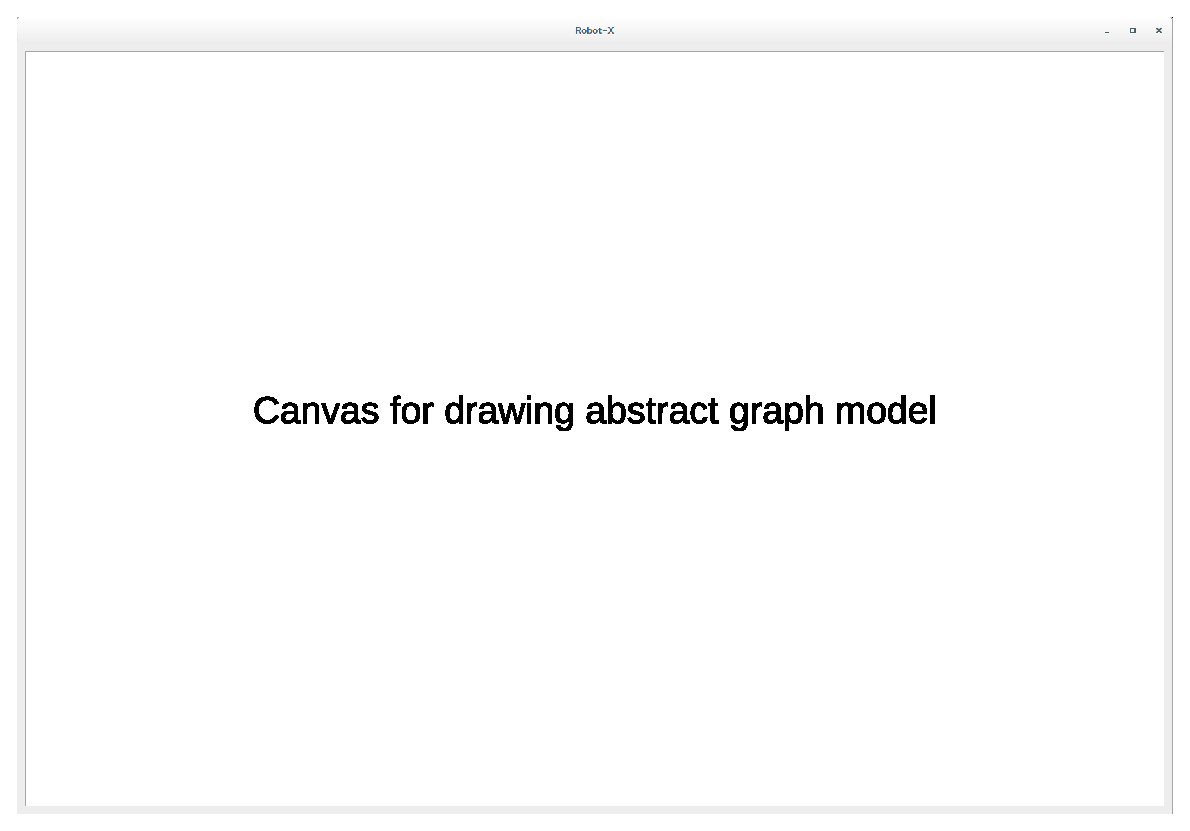
\includegraphics[width=0.32\textwidth]{img/RobotXUI.eps}
  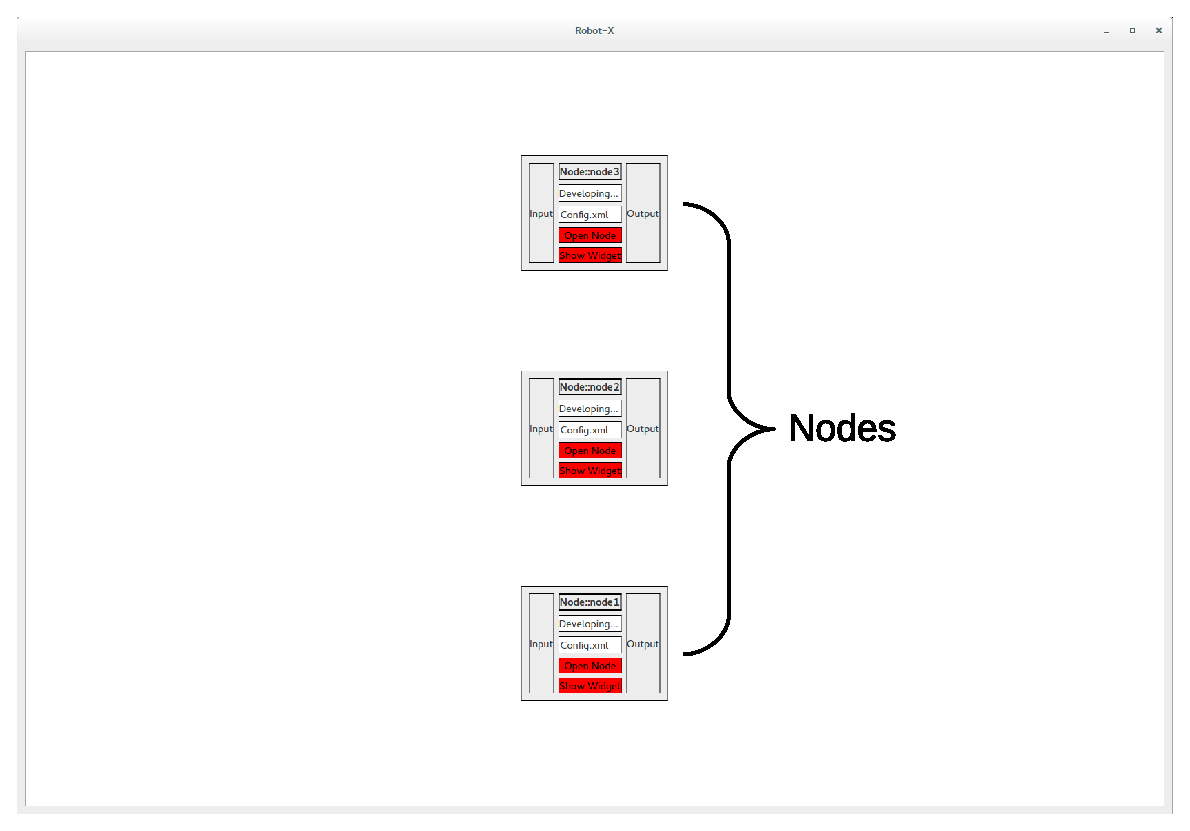
\includegraphics[width=0.32\textwidth]{img/RobotXnode.eps}
   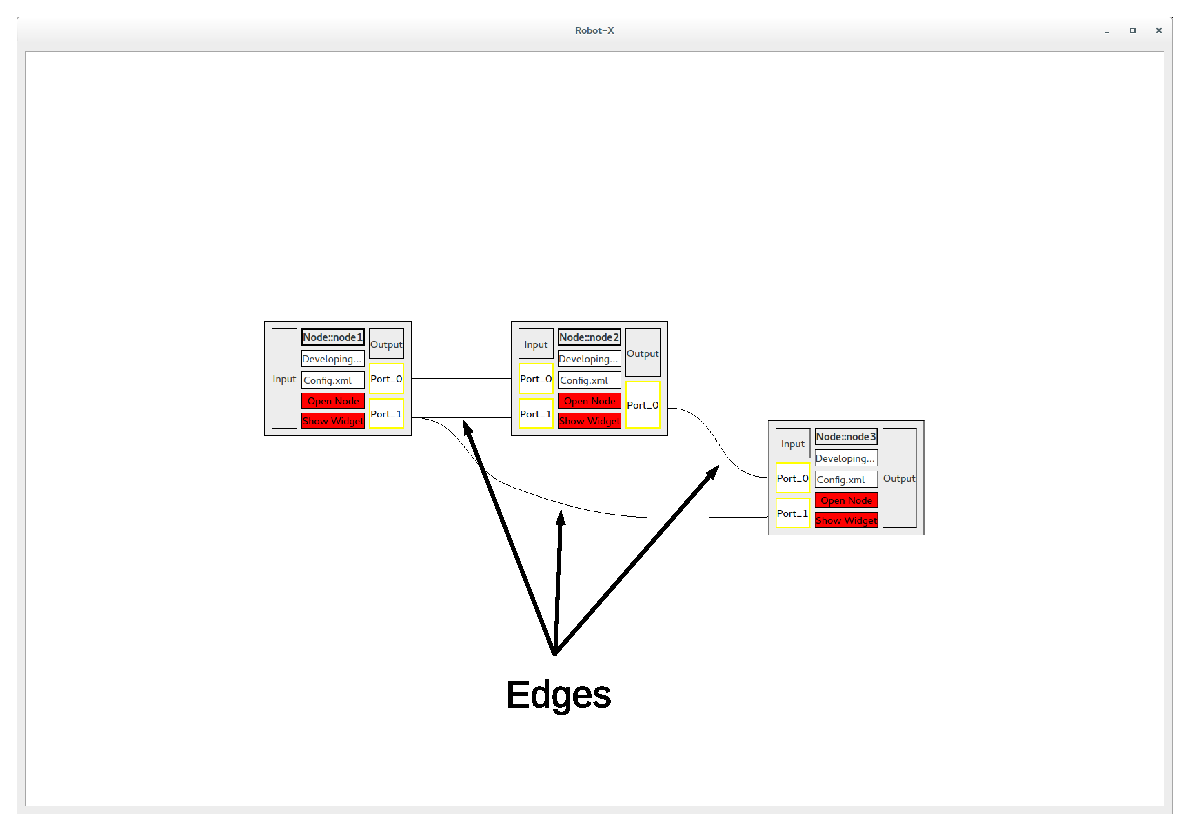
\includegraphics[width=0.32\textwidth]{img/RobotXedge.eps}
 \caption{Robot-X UI}
 \label{fig:robotxui}
\end{figure}

\subsection{Node}

\subsubsection{Add Node}

To add a node, right click on the empty part of the canvas and a menu pop up as Fig.\ref{fig:addnode} left. There are two kinds of node you can add to the graph: virtual node and real node. The virtual node is an abstract node, whose functional module has not been developed. But it can still be included in the abstract graph model and this is the key for top-down development. The real node's functional module has been compiled in some shared libraries, which should be loaded after creating the node as Fig. \ref{fig:addnode} right.

\begin{figure}
 \centering
 \includegraphics[width=1.0\textwidth]{img/addnode.eps}
 \caption{Add Virtual Node and Real Node Operations}
 \label{fig:addnode}
\end{figure}

As shown in the middle of Fig.\ref{fig:addnode}, in order to create a node, you need to give it a {\em{"Node Full Name"}}. The name rule is: 

\begin{framed}
\centering
NodeClass::NodeName[::ExName]
\end{framed}

The "NodeClass" of a node is one part of query ID for RobotSDK to locate its functional module in shared library. For each module, it should have a unique "NodeClass" in one shared library. The "NodeName" could be any name you want to instantiate a "NodeClass". The "ExName" is optional and is another part of the query ID for RobotSDK to locate the module's extended functionality in the shared library. In a graph model, users only need to guarantee the uniqueness of "Node Full Name".

\subsubsection{Virtual Node and Real Node}

After adding either virtual or real node, it will be included in the graph as shown in the middle of Fig.\ref{fig:robotxui}. From Fig.\ref{fig:node}, we could find that the only differences between new created virtual and real nodes are 1) input or output ports and 2) shared library. The virtual node does not have any input or output ports and the shared library is still in "Developing...". The real node has input or output ports which is defined in the functional module from a certain shared library.

\begin{figure}
 \centering
 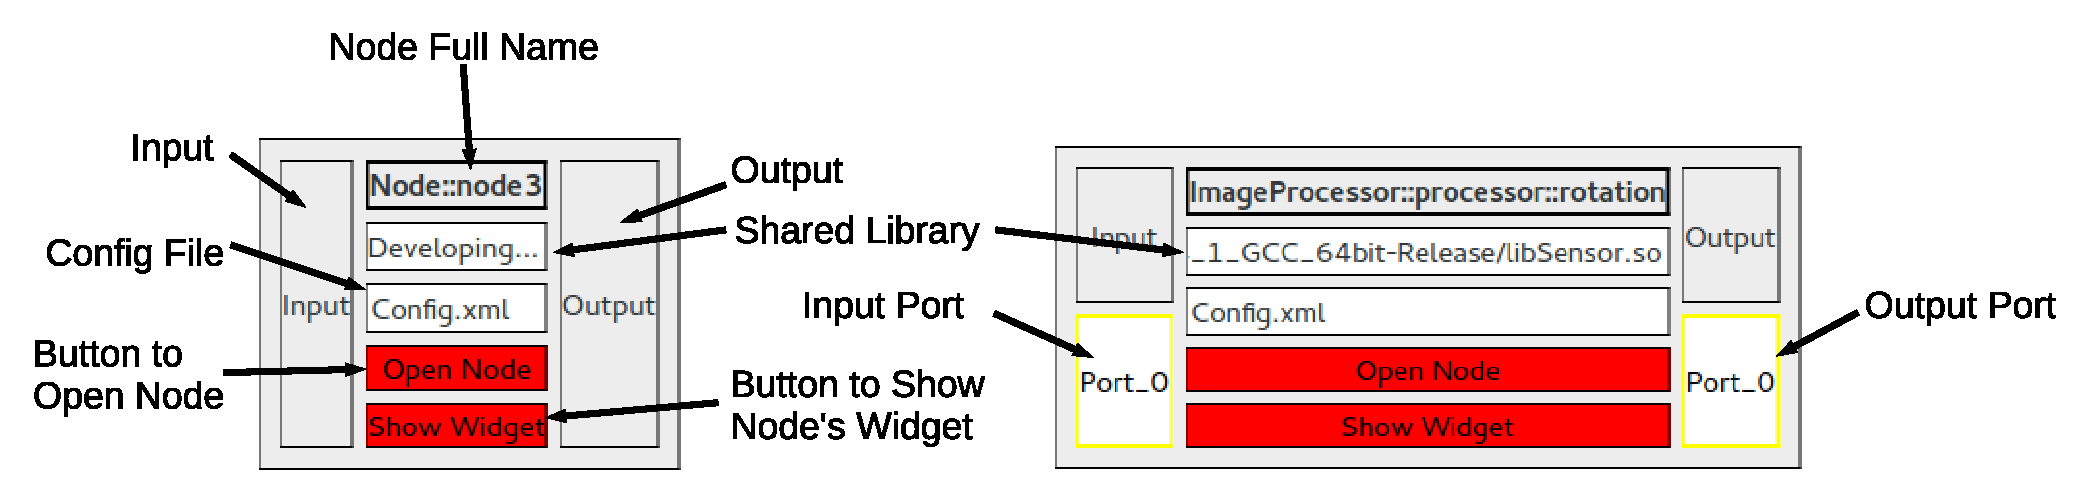
\includegraphics[width=1.0\textwidth]{img/node.eps}
 \caption{New Virtual Node (Left) and Real Node (Right) in Abstract Graph Model}
 \label{fig:node}
\end{figure}

\subsubsection{Set Port Number}

After adding virtual node, it does not have both input and output ports as shown in Fig.\ref{fig:node} left, and users need to to set the input and output port number. To set port number, right click on the "Input" or "Output" label and a menu pop up as Fig.\ref{fig:addport} left. Then choose "Change Port Num" and a dialog for setting port number is shown. After setting the port number and click "OK", the ports will be added to the virtual node as Fig.\ref{fig:node} right. After change port number, you will find a "Input" or "Output" label with black frame on the top and several "Port\_x" labels with yellow frame below.

\begin{figure}
 \centering
 \includegraphics[width=0.8\textwidth]{img/addport.eps}
 \caption{Set Port Number}
 \label{fig:addport}
\end{figure}

For real node, it is compatible to change its port number and there will not be any problems while running the software. However, if the new port number is larger than defined one, the exceeded ports will only act as an abstract ports, which convert the real node to be a semi-real or semi-virtual node. If the new port number is smaller than defined one, the lost ports will not appear in the abstract graph model and thus are not available for the software, which only means no input or output for the lost ports. 

\subsubsection{Change Shared Library}

According to the principle of top-down software development, virtual node does not have functional module and corresponding shared library at the beginning. Then, after abstract graph model construction and functional module development, the virtual node should turn to a real node, which is to change the shared library from "Developing..." to real one. To change shared library, right click on the "Node Full Name" label and a menu pop up as Fig.\ref{fig:changelibrary} top-left. Then choose "Change Library" and an open file dialog is shown to load shared library just like adding real node operation. The only thing you must guarantee is that the loaded shared library contains the module with desired "NodeClass" (and "ExName").

According to the principle of modular software development, a real node is an interface in which various modules with similar functionalities could embed. Therefore, Robot-X also allows users to change shared library for real node. The operation is same to that for virtual node as Fig.\ref{fig:changelibrary} bottom-left. RobotSDK supports hot-plug of shared library, which means you need not to restart application for changing shared library. However, there is a very important thing, to which the users must pay attention:

\begin{framed}
RobotSDK uses QLibrary to load shared library. Once a shared library is loaded, it will not be destroyed until the application exists and thus the shared library with same name will not be loaded again. Therefore, if you modify a loaded shared library, the modification will not be applied unless you restart the application. 
\end{framed}

\begin{figure}
 \centering
 \includegraphics[width=0.8\textwidth]{img/changelibrary.eps}
 \caption{Change Shared Library of Virtual and Real Nodes}
 \label{fig:changelibrary}
\end{figure}

\subsubsection{Change ExName}

The "ExName" is a part of query ID for RobotSDK to locate its module's extended functionalities. Therefore, once a node is created, you could and only could change the "ExName" of the "Node Full Name" to use different extended functionalities. For example, as shown in Fig.\ref{fig:exname}, the "ImageProcessor" base module is to consecutively rotate, scale and enhance an input image and output the processed image. However, these three steps are not always needed. Therefore, we extend it as "ImageProcessor::--::rotation", "ImageProcessor::--::scale" and "ImageProcessor::--::enhance". Here, we stress that, these three extensions are not new modules, they are still in base module "ImageProcessor" and their input and output are same with base module "ImageProcessor". The only difference is the "main function" are different (see Chapter \ref{module}).

\begin{figure}
 \centering
 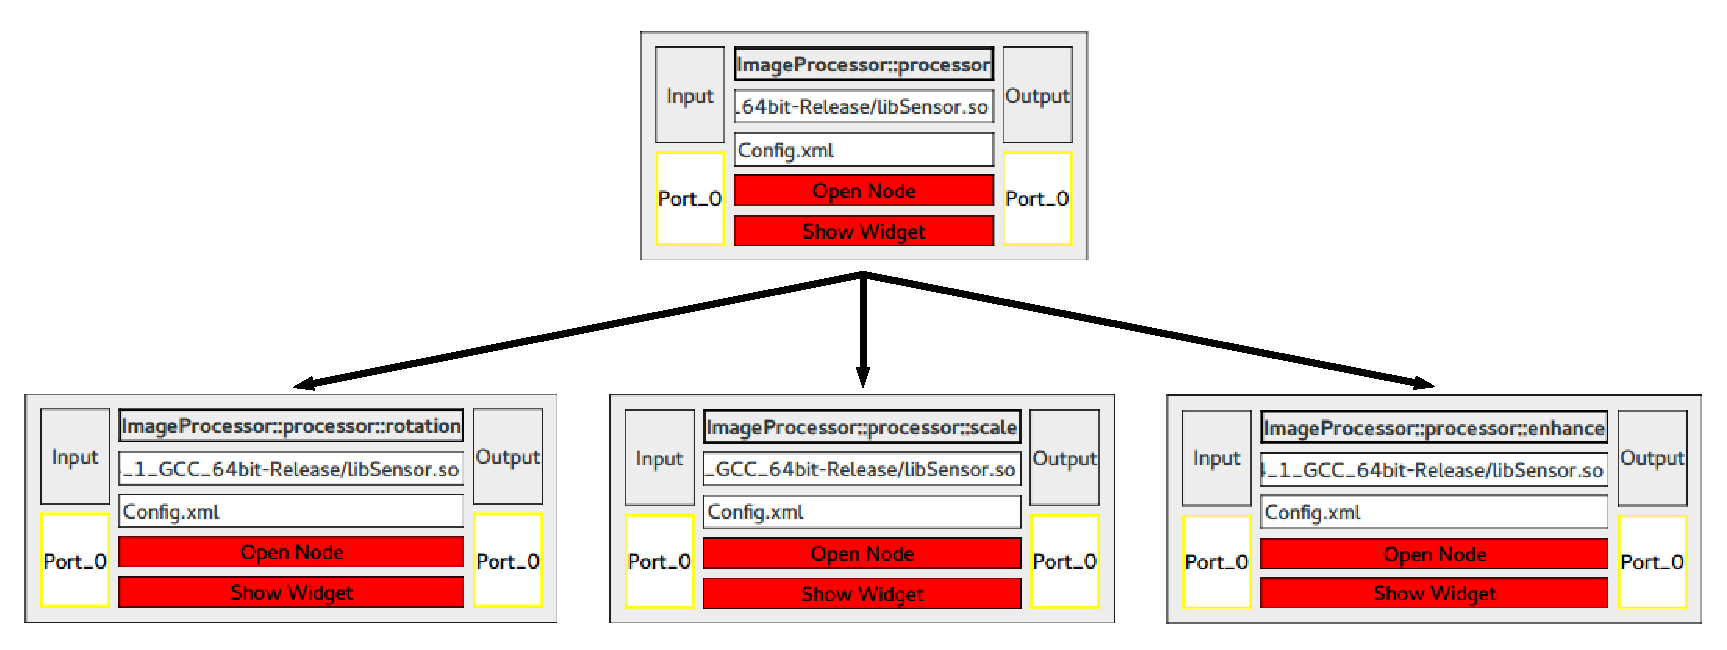
\includegraphics[width=1.0\textwidth]{img/exname.eps}
 \caption{Extension of Module "ImageProcessor"}
 \label{fig:exname}
\end{figure}

To change the "ExName", right click on the "Node Full Name" label and a menu pop up as shown in Fig.\ref{fig:changeexname} left. Then choose "Change ExName" and a dialog to change "ExName" is shown. Click "OK" after changing, the node changes its "ExName". In the example, the changing is from real node's base module "ImageProcessor" to extension "ImageProcessor::--::rotation". The first thing to be clarified is that the changing from extension to base module or among module's extensions is also available. The second thing is that for virtual node, the changing of "ExName" is also available and it is just the modification of abstract graph model. The third thing is that for real node, the changing of "ExName" will automatically load desired modules.

\begin{figure}
 \centering
 \includegraphics[width=1.0\textwidth]{img/changeexname.eps}
 \caption{Change ExName of Module "ImageProcessor"}
 \label{fig:changeexname}
\end{figure}

\subsubsection{Change Config File and Values}

Just as RobotSDK 3.0, each node is related to a configuration file in XML format. In RobotSDK 4.0, Robot-X provides a way to change configuration file. To change the "Config File", right click on the "Node Full Name" label and a menu pop up as shown in Fig.\ref{fig:changeconfig} left. Then choose "Change Config File" and an open file dialog is shown to change "Config File". Click "Open" will change node's "Config File". In order to apply the new configuration file, you need to reopen the node, because as shown in Fig.\ref{fig:nodestate}, the configuration file will be loaded in "Initialize Node" and "Open Node" states.

\begin{figure}
 \centering
 \includegraphics[width=0.8\textwidth]{img/changeconfig.eps}
 \caption{Change Configuration File}
 \label{fig:changeconfig}
\end{figure}

In RobotSDK 3.0, users need to manually change XML file contents to realize modification of parameters. In RobotSDK 4.0, Robot-X provides a UI to modify parameters stored in XML file as shown in Fig.\ref{fig:changeconfigvalues} middle. To change the "Config Values", right click on the "Node Full Name" label and a menu pop up as shown in Fig.\ref{fig:changeconfigvalues} left. Then choose "Change Config Values" and a table dialog is shown to modify parameters.  After modification, click "OK" for save \& close, click "Apply" only for save and click "Cancel" for abort \& close. There are two types of parameters modification: 1) Change value via "QLineEdit" and 2) Choose value via "QComboBox". The corresponding contents in XML file are shown in Fig.\ref{fig:changeconfigvalues} right. To register such parameters, please see Chapter \ref{module}.

\begin{figure}
 \centering
 \includegraphics[width=0.8\textwidth]{img/changeconfigvalues.eps}
 \caption{Change Configuration Values}
 \label{fig:changeconfigvalues}
\end{figure}

\subsubsection{Generate Code}

Just like RobotSDK 3.0's ConfigModule tool, Robot-X could generate interface code for module development after setting up node. To generate code, right click on the "Node Full Name" label and a menu pop up as shown in Fig.\ref{fig:generatecode} top-left. Then choose "Generate Code" and a path open dialog is shown to decide where to store code files. After choosing desired path and clicking open, two code files named as "NodeClass" will be generated as Fig.\ref{fig:generatecode} bottom-left and their contents are shown in Fig.\ref{fig:code}. In the source file, there are four predefined functions: "initializeNode", "openNode", "closeNode" and "main". Their correspondences to Node State in Fig.\ref{fig:generatecode} bottom-right are: "Initialize Node", "Open Node", "Close Node" and "Execution". How to program the interface code please see Chapter \ref{module}.

\begin{figure}
 \centering
 \includegraphics[width=0.7\textwidth]{img/generatecode.eps}
 \caption{Generate Interface Code for Module Development}
 \label{fig:generatecode}
\end{figure}

\begin{figure}
 \centering
 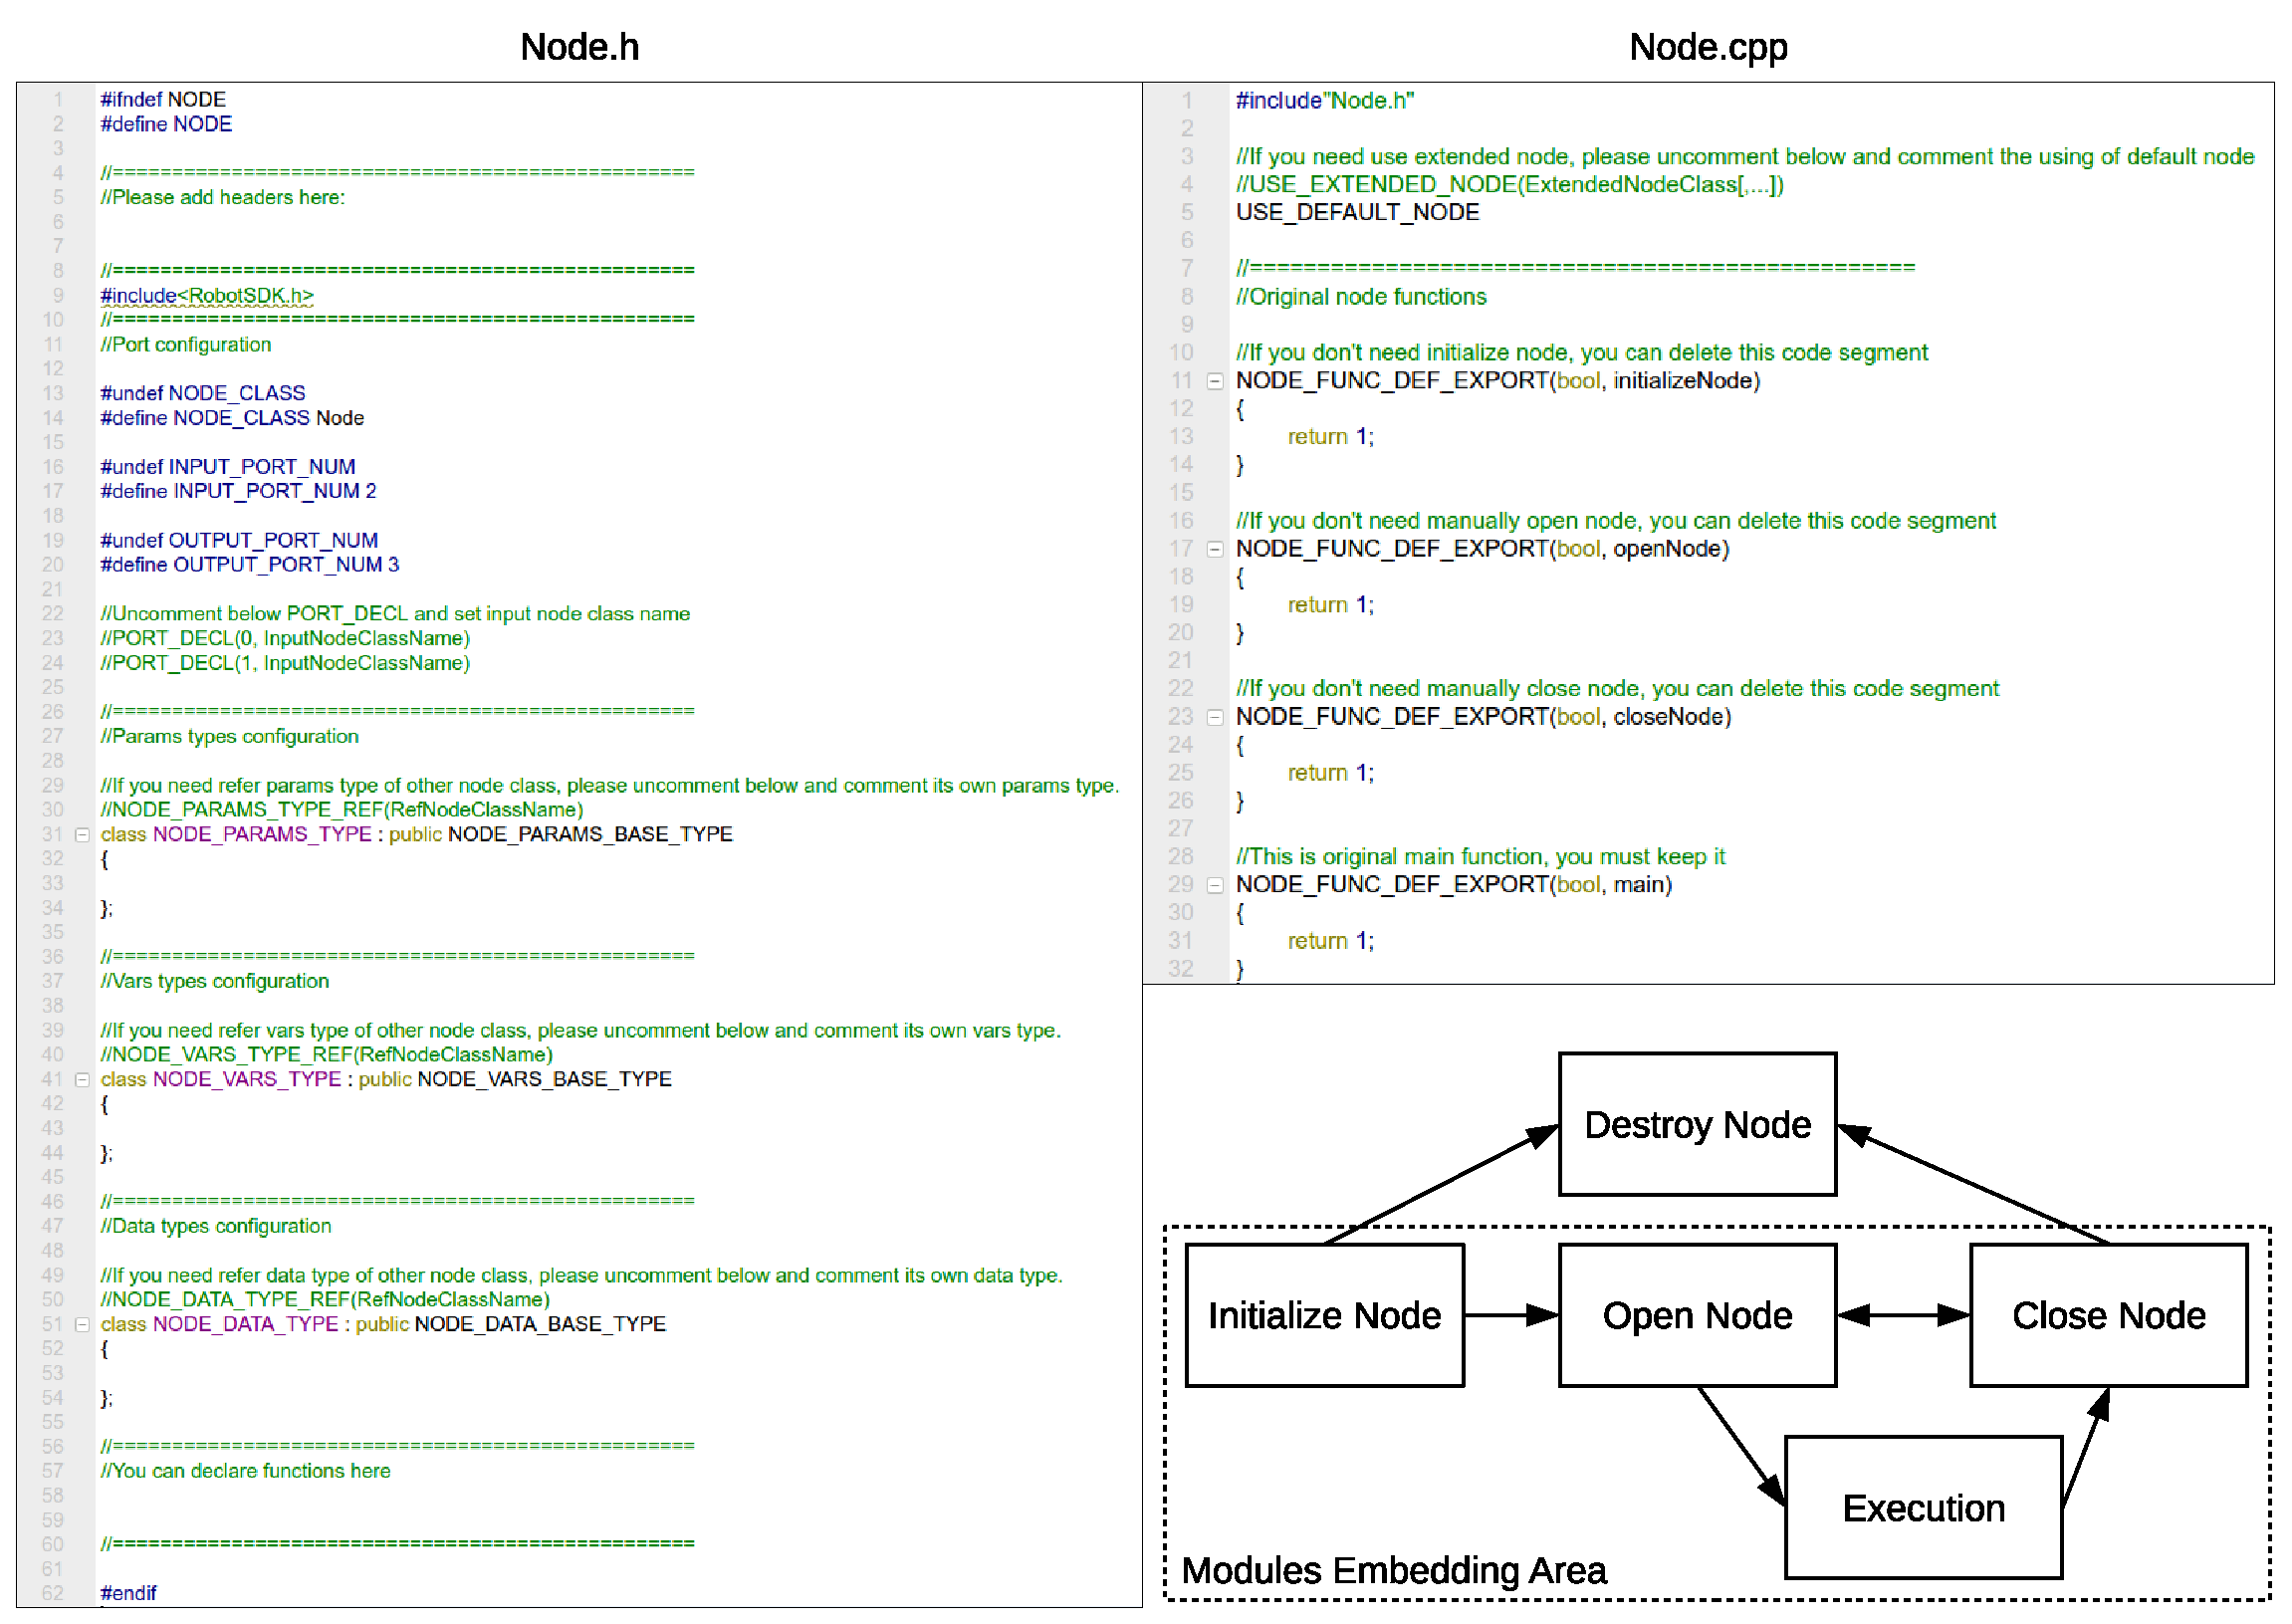
\includegraphics[width=1.0\textwidth]{img/code.eps}
 \caption{Contents of Interface Code and Their Correspondences to Node State}
 \label{fig:code}
\end{figure}

\subsubsection{Delete Node}

To delete a node, right click on the "Node Full Name" label and a menu pop up as shown in Fig.\ref{fig:deletenode} top. After choosing "Delete Node", the selected node will be deleted from the abstract graph mode, as well as its connected edges and communications with other nodes.

\begin{figure}
 \centering
 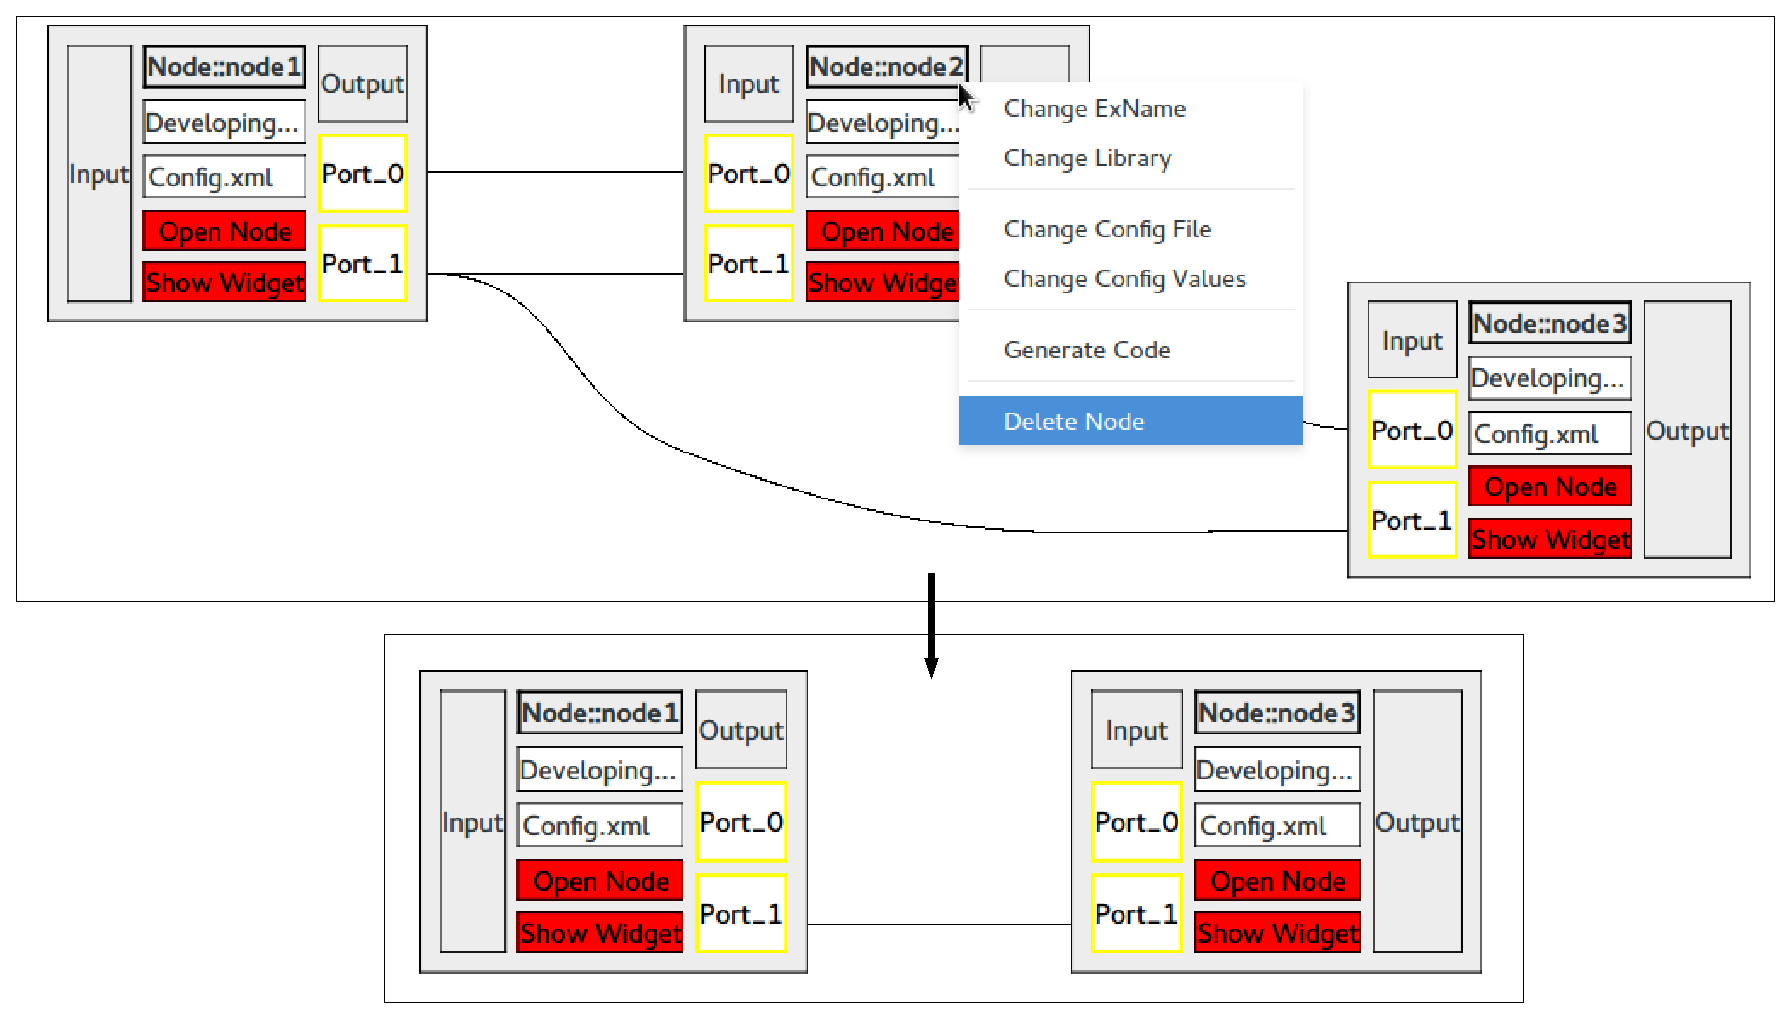
\includegraphics[width=0.7\textwidth]{img/deletenode.eps}
 \caption{Delete Node from Abstract Graph Model}
 \label{fig:deletenode}
\end{figure}

\subsection{Edge}

\subsubsection{Add an Edge}

Edge in abstract graph model is to connect a pair of output port and input port in different nodes or in same node (loop, feedback). Robot-X provides a drag-n-drop operation for users to interactively add edge as shown in Fig.\ref{fig:dragdrop}. When mouse moves into a port, its cursor turns to open-hand shape (Fig.\ref{fig:dragdrop} top-left). When press mouse left button, a port drag instance will be created as a transparent text box with port information (Fig.\ref{fig:dragdrop} top-right). When move the port drag instance into a correct port (input $\leftrightarrow$ output), the latter one will turn to green, which means ready to be linked, and then an edge will be added if drop the former one (Fig.\ref{fig:dragdrop} bottom-left). When move the port drag instance into a wrong port, the latter one will turn to red and no edge will be added (Fig.\ref{fig:dragdrop} bottom-right). Fig.\ref{fig:addedge} illustrates complete operations to add an edge between corresponding ports. 

[Update-150427] When you put mouse on a port of node, a toolkit will show the related "NodeClass".

\begin{figure}
 \centering
 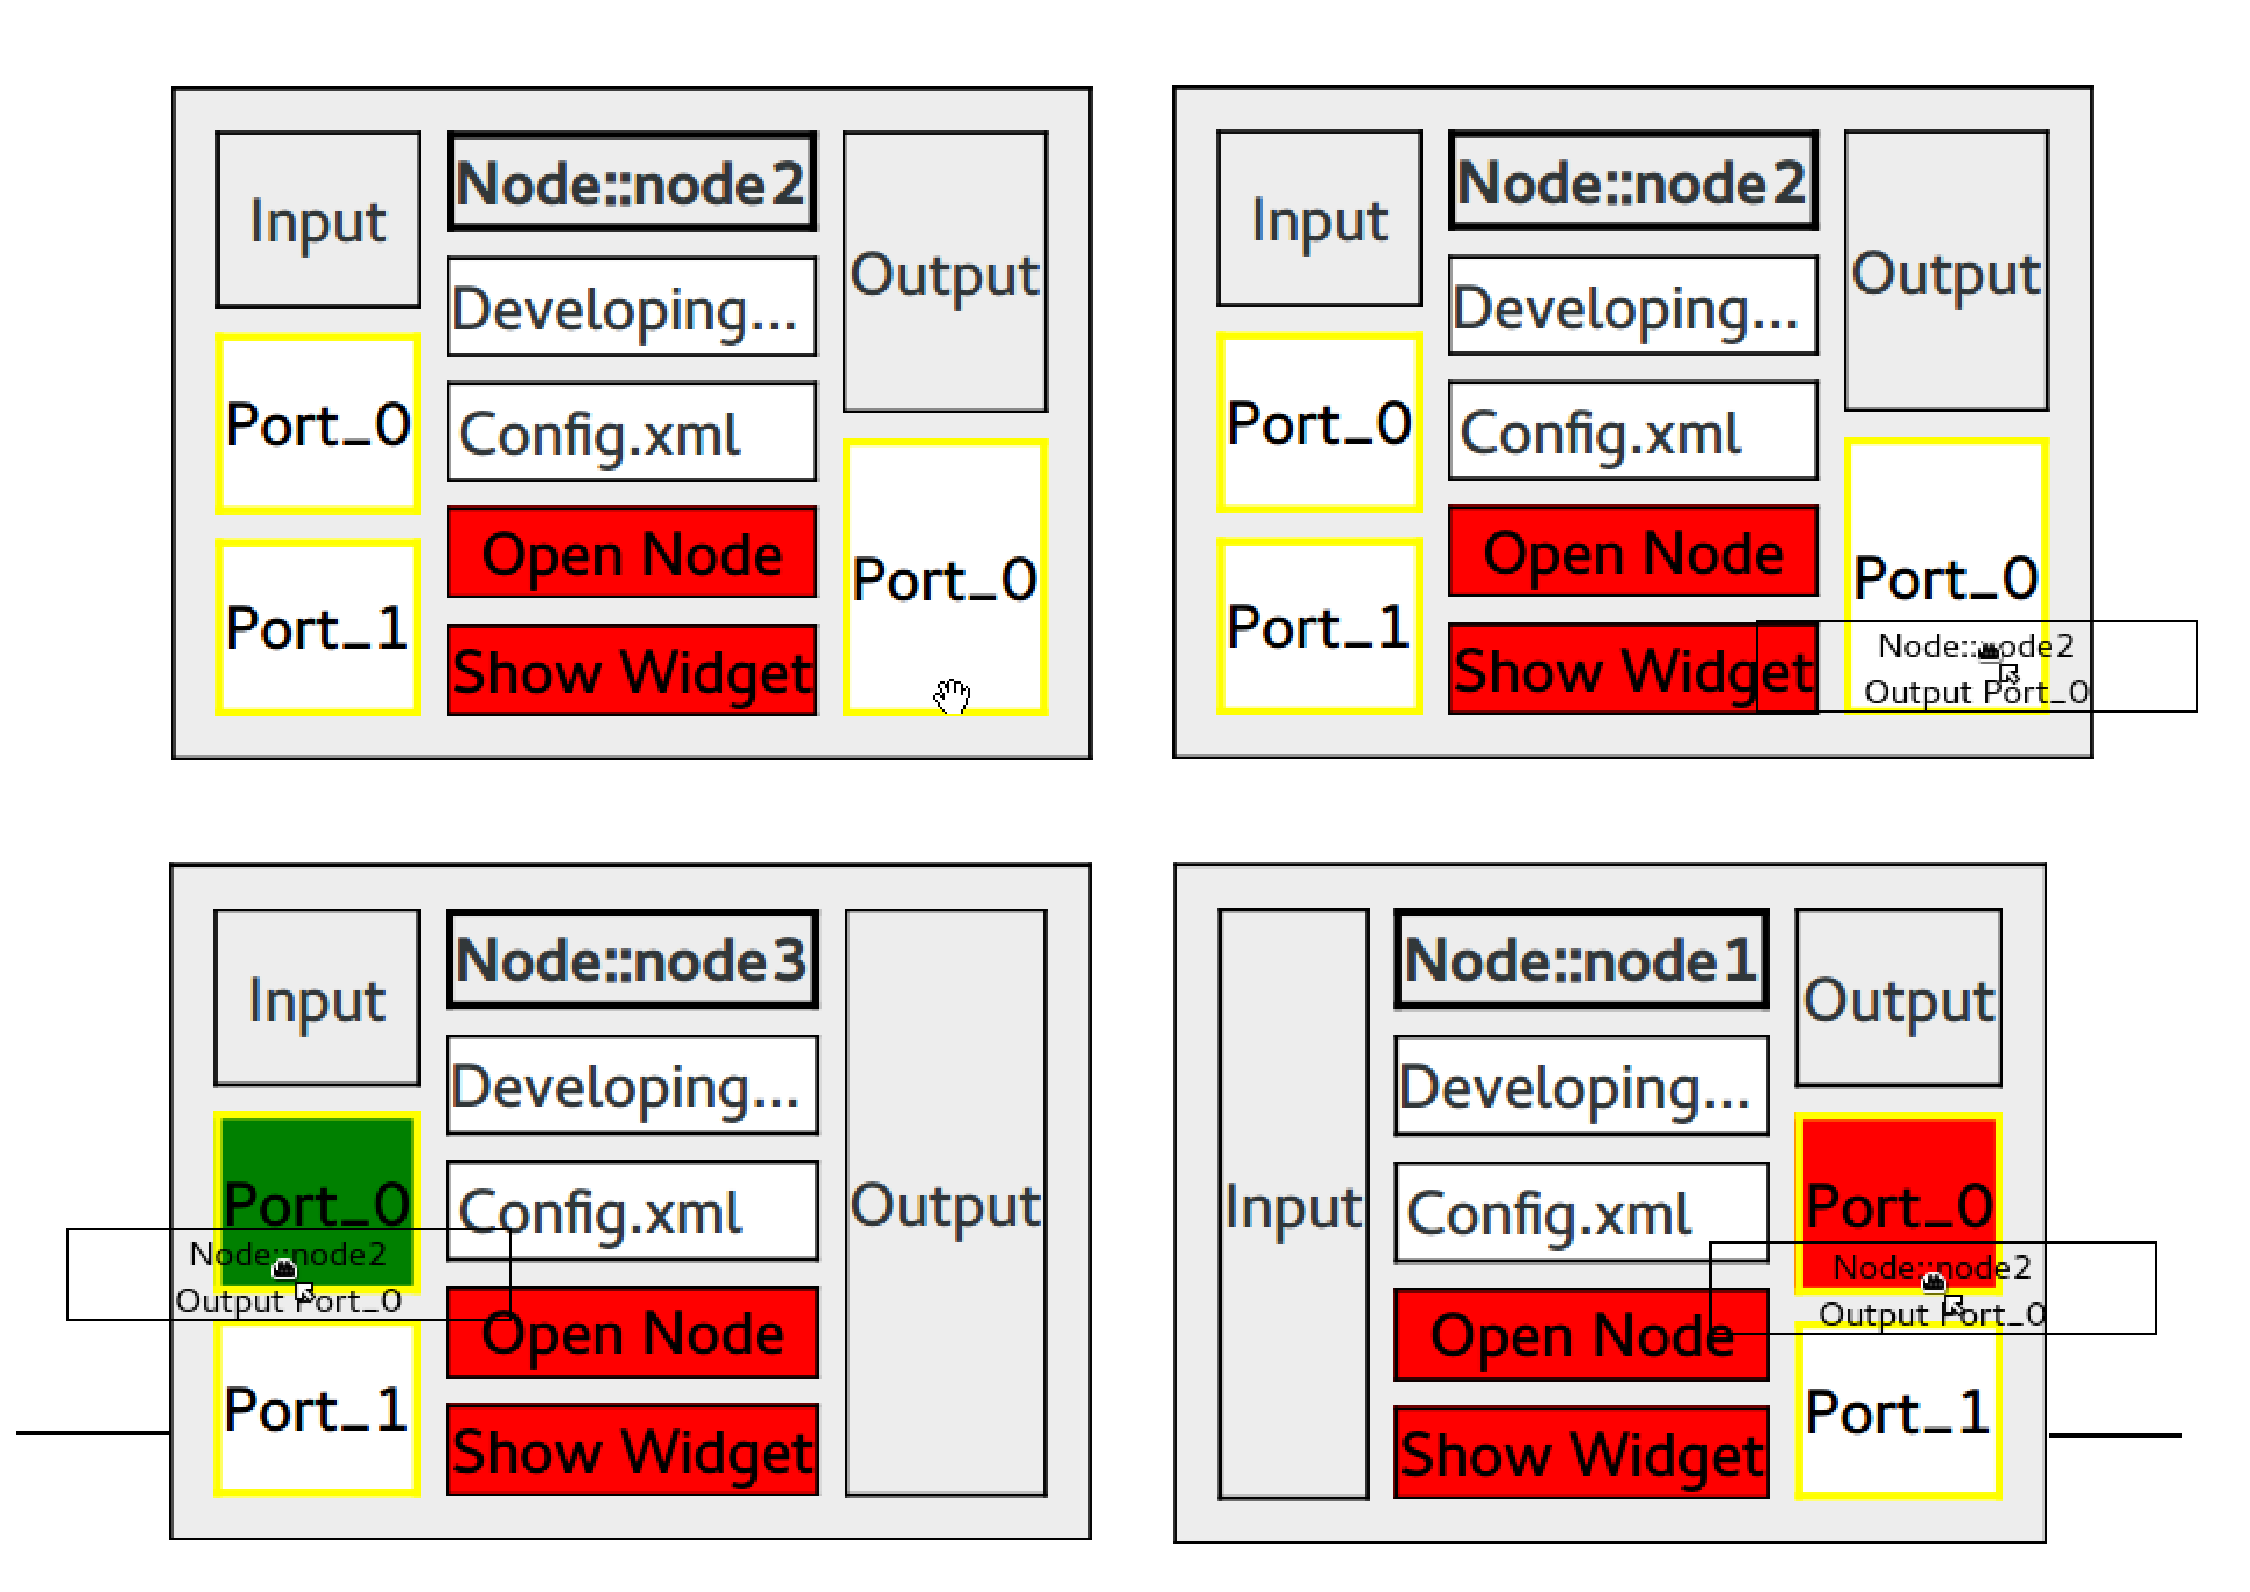
\includegraphics[width=0.6\textwidth]{img/dragdrop.eps}
 \caption{Drag-n-Drop Operation}
 \label{fig:dragdrop}
\end{figure}

\begin{figure}
 \centering
 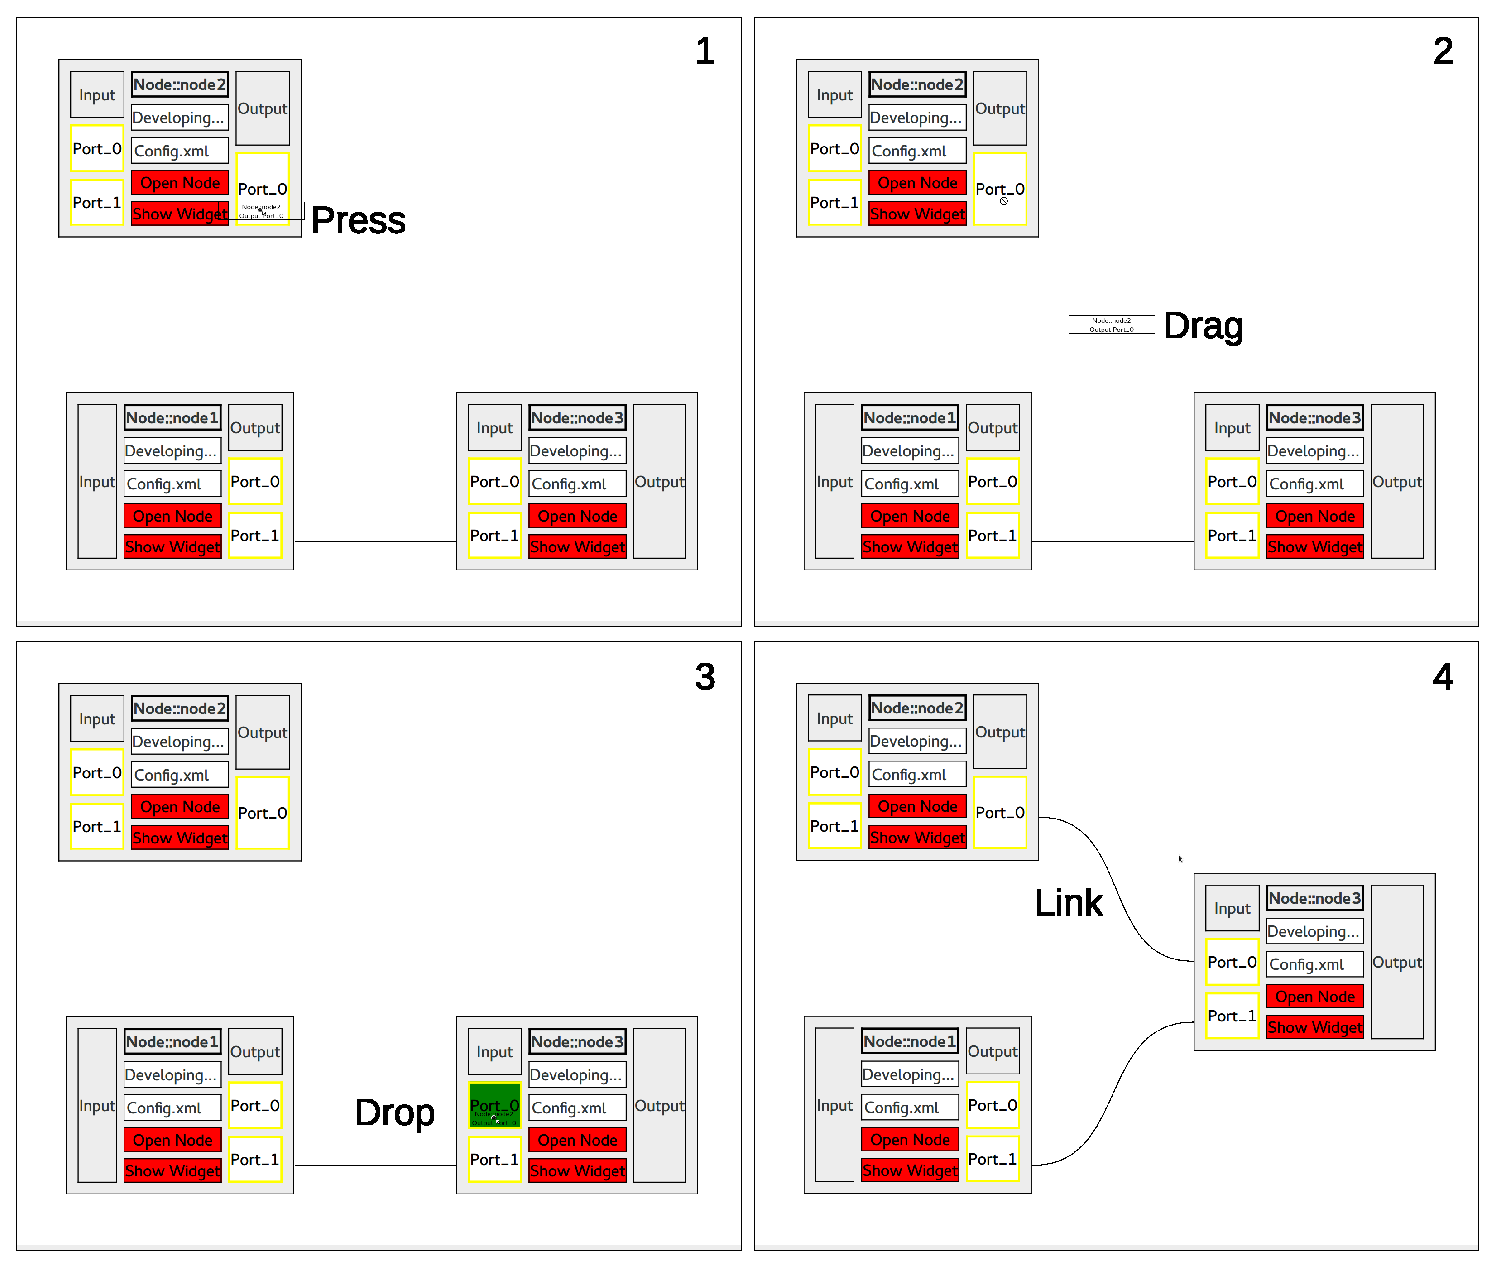
\includegraphics[width=0.8\textwidth]{img/addedge.eps}
 \caption{Complete Operations to Add an Edge}
 \label{fig:addedge}
\end{figure}

If an edge connects two real nodes, then the communication (signal-slot inter-thread connection) between these two ports will be automatically built. Otherwise (include semi-virtual node), the edge only appears in abstract graph model. Once a virtual or semi-virtual node turns to a real node by changing shared library, Robot-X will automatically check its related edges to build communications with other real nodes. Both edges in abstract graph model and communications will be kept after changing shared library or "ExName" of real node.  

\subsubsection{Check an Edge}

The organization of graph model is conducted by GraphViz, which tries its best to optimize edge-crossing. However, complex graph will indeed generate a mass of edges. Therefore, Robot-X provides a way to check edge's information and path as shown in Fig.\ref{fig:checkedge}. When mouse moves on an edge, its cursor turns to open-hand shape and a tooltip will appear to show edge's information (Fig.\ref{fig:checkedge} top). When press mouse left button, the edge's path will turn to red for clear identification (Fig.\ref{fig:checkedge} bottom).

\begin{figure}
 \centering
 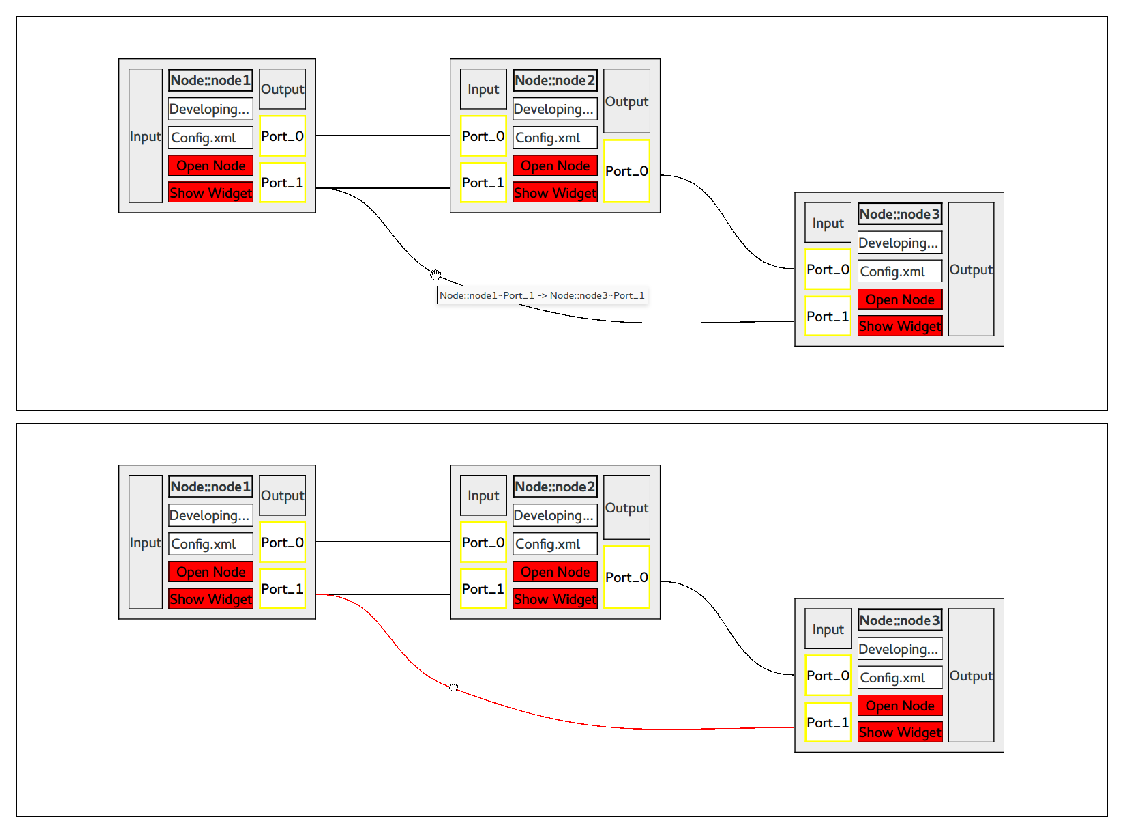
\includegraphics[width=0.8\textwidth]{img/checkedge.eps}
 \caption{Check Edge's Information and Path}
 \label{fig:checkedge}
\end{figure}

\subsubsection{Delete an Edge}

To delete an edge, right click on the checked edge and a menu pop up as shown in Fig.\ref{fig:deleteedge} top. After selecting "Delete Edge", the edge will be removed from abstract graph model as Fig.\ref{fig:deleteedge} bottom. If the edge corresponds to a communication, the communication will be disconnected automatically.

\begin{figure}
 \centering
 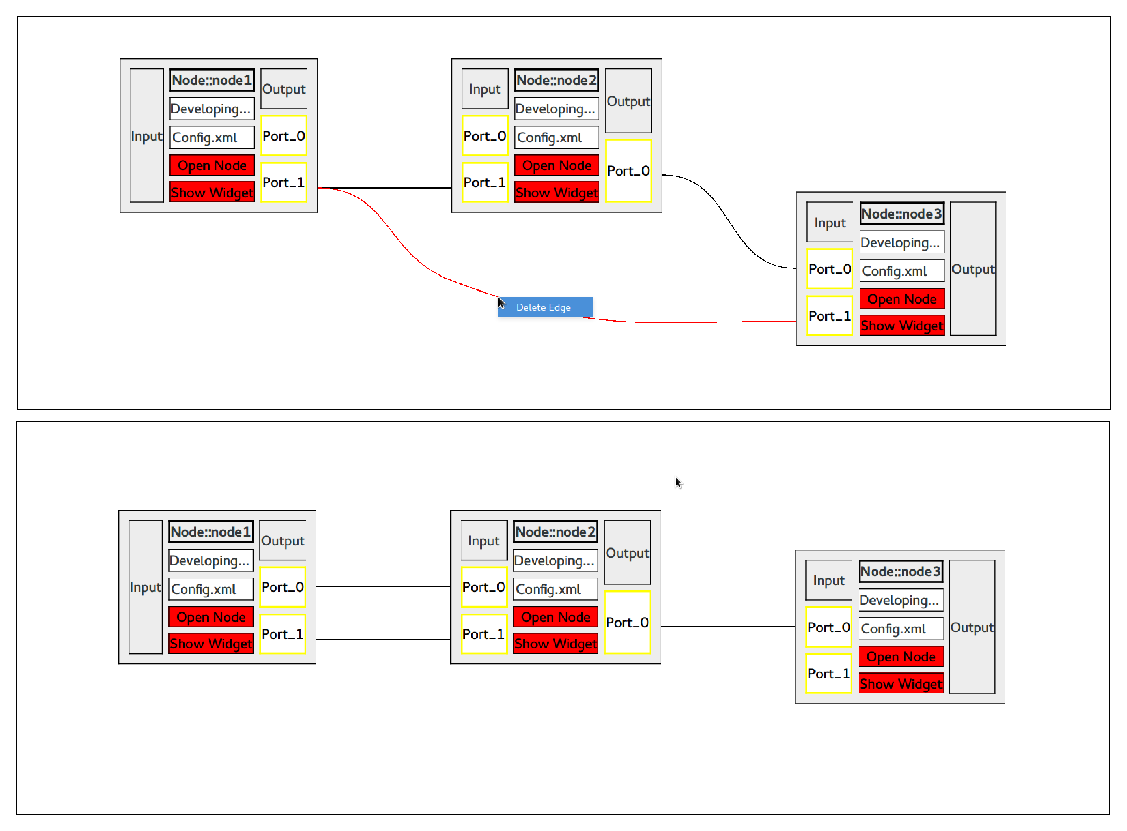
\includegraphics[width=0.8\textwidth]{img/deleteedge.eps}
 \caption{Delete Edge}
 \label{fig:deleteedge}
\end{figure}

\subsection{Graph}

\subsubsection{Save and Load a Graph}

When you have finished an abstract graph model, you hope to store it as a file for further development, sharing with collaborators or launching software quickly. Robot-X provides functions for saving and loading abstract graph model. 

Right click on the empty part of Robot-X canvas and a menu pop up as shown in Fig.\ref{fig:saveloadgraph} top-left. To save a graph, choose "Save Graph" and then a file save dialog appears. The graph file's suffix is .x and the contents are shown in Fig.\ref{fig:saveloadgraph} bottom-left. The graph file contains two parts: 1) nodes description and 2) edges description. For node description, there are 5 values except for the first identifier 'N': 1) Node Full Name, 2) Shared library (empty for virtual node), 3) Configuration file, 4) Input ports number and 5) Output ports number. For edge description, there are 4 values except for the first identifier 'E': 1) Output Node Full Name, 2) Output port ID, 3) Input Node Full Name and 4) Input port ID.

To load a graph, choose "Load Graph" and then a file load dialog appears. You can load any numbers of graph files into Robot-X and a graph union operation will be performed after loading as shown in Fig.\ref{fig:graphunion}. This could be used to merge many sub-systems into one system. RobotSDK 4.0 uses constant shared\_ptr to protect output data, therefore, nodes with same Node Full Name in different sub-systems could be safely merged as one node. 

\begin{figure}
 \centering
 \includegraphics[width=1.0\textwidth]{img/saveloadgraph.eps}
 \caption{Save and Load a Graph. The Contents of Graph File}
 \label{fig:saveloadgraph}
\end{figure}

\begin{figure}
 \centering
 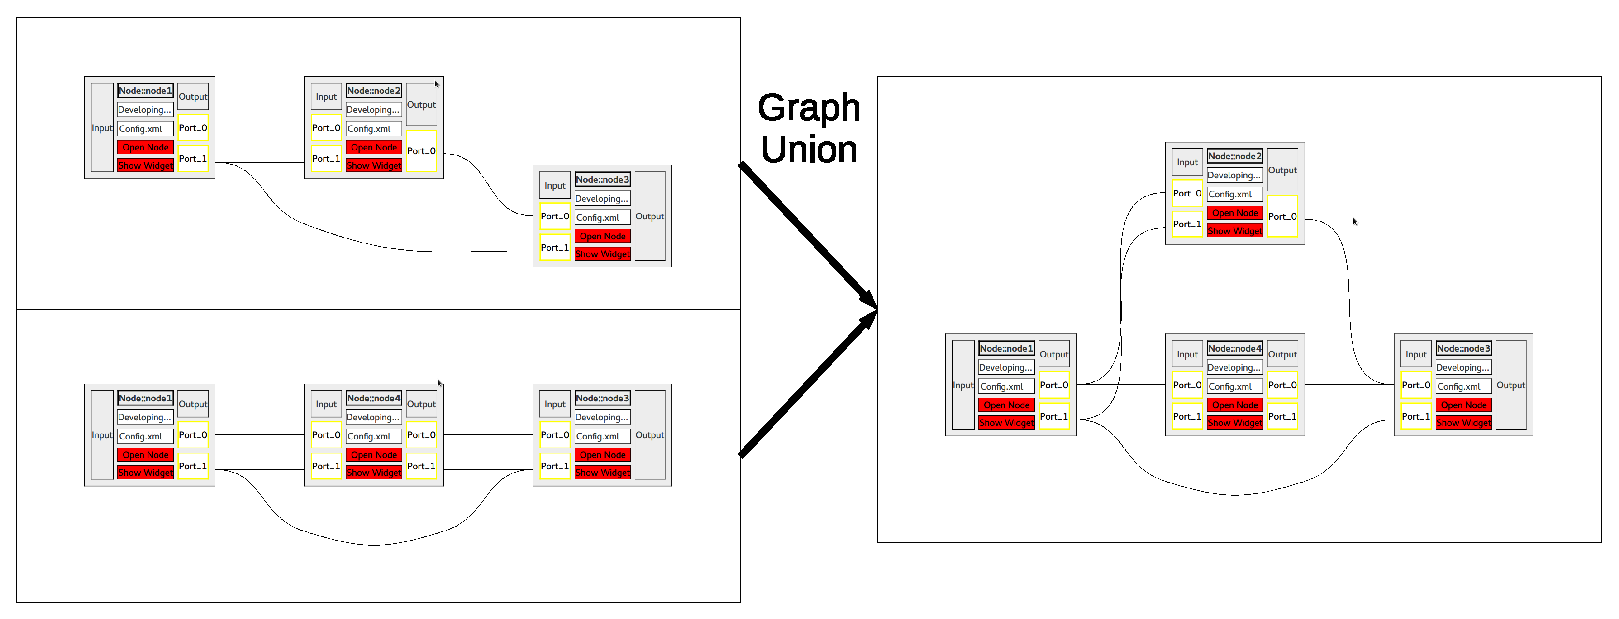
\includegraphics[width=1.0\textwidth]{img/graphunion.eps}
 \caption{Graph Union by Loading Two Graph Files into Same Graph Model}
 \label{fig:graphunion}
\end{figure}

\subsubsection{Export Graph Image and Dot File}

Sometimes, it is desirable to output standard image of abstract graph model for presentation of publishing. Robot-X uses GraphViz to render .png image file as shown in Fig.\ref{fig:sample}. To export graph image file, right click on empty part of Robot-X canvas and a menu pop up as shown in Fig.\ref{fig:exportimage} left. Choose "Export Graph Image..." and a save file dialog appears. After saving, a image file is stored as Fig.\ref{fig:exportimage} bottom-right.

\begin{figure}
 \centering
 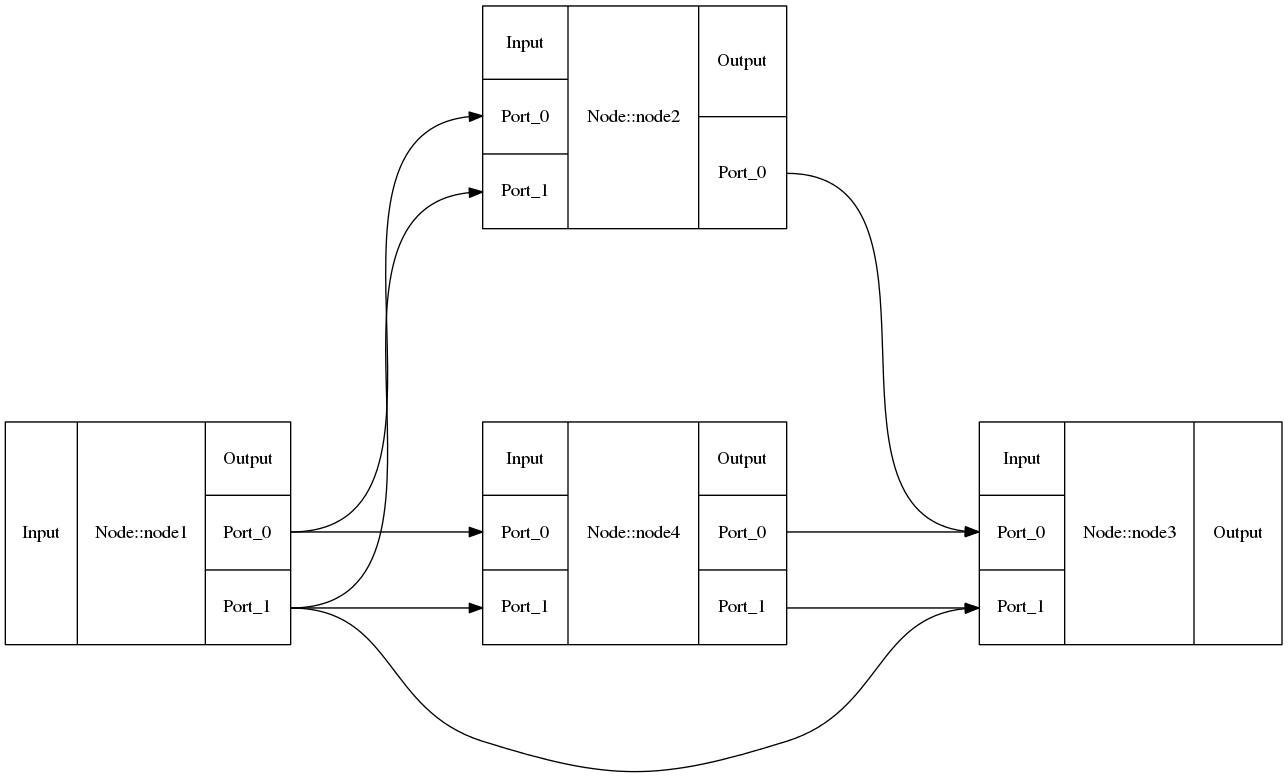
\includegraphics[width=0.8\textwidth]{img/sample.png}
 \caption{Image File of Graph Union Example}
 \label{fig:sample}
\end{figure}

\begin{figure}
 \centering
 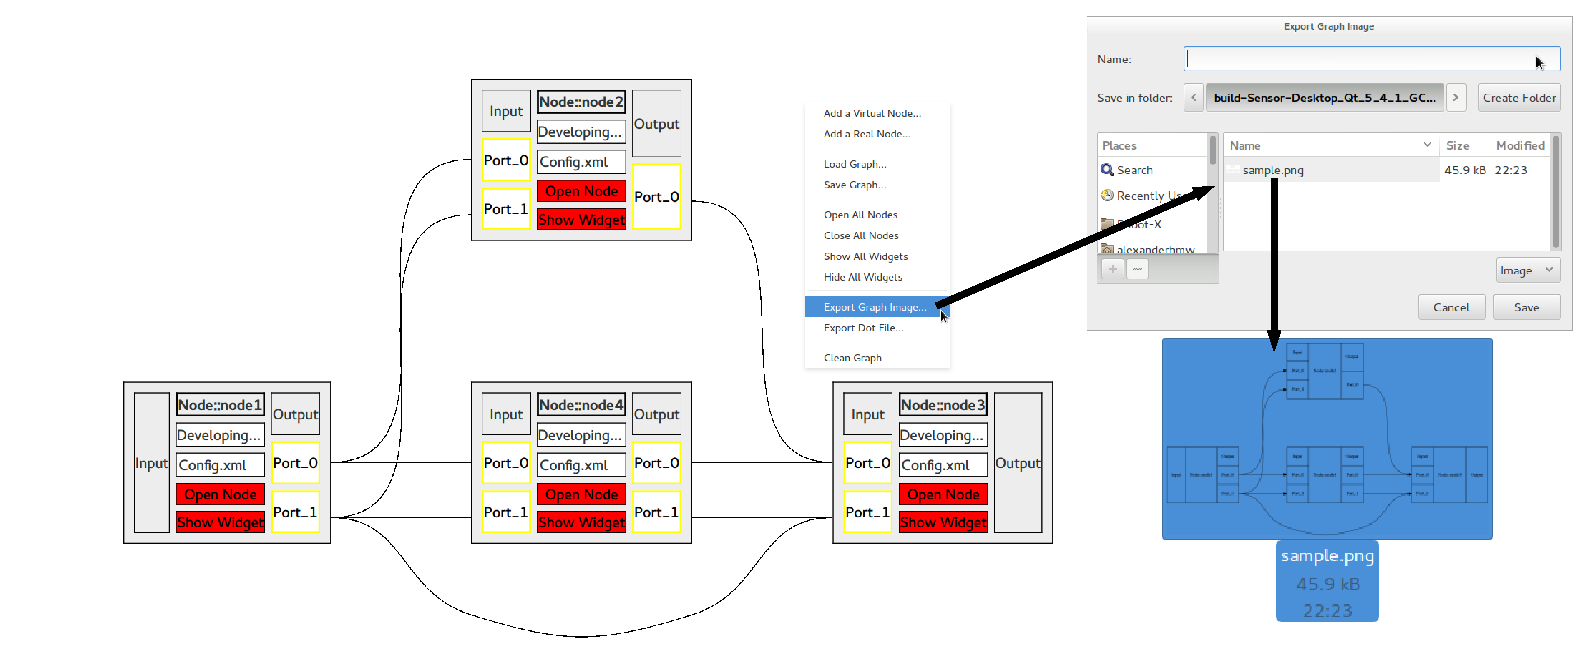
\includegraphics[width=1.0\textwidth]{img/exportimage.eps}
 \caption{Export Graph Image of Abstract Graph Model}
 \label{fig:exportimage}
\end{figure}

Dot file is a popular graph file type and most graph-related applications could read it. For example, here is a website [\url{http://graphs.grevian.org/graph}] which reads dot file contents and draw the graph as shown in Fig.\ref{fig:dotfile}. To export dot file, right click on empty part of Robot-X canvas and a menu pup up as shown in Fig.\ref{fig:exportdot} top-left. Choose "Export Dot File..." and a save file dialog appears. After saving, a dot file is stored and its contents are shown in 
Fig.\ref{fig:exportdot} right.

\begin{figure}
 \centering
 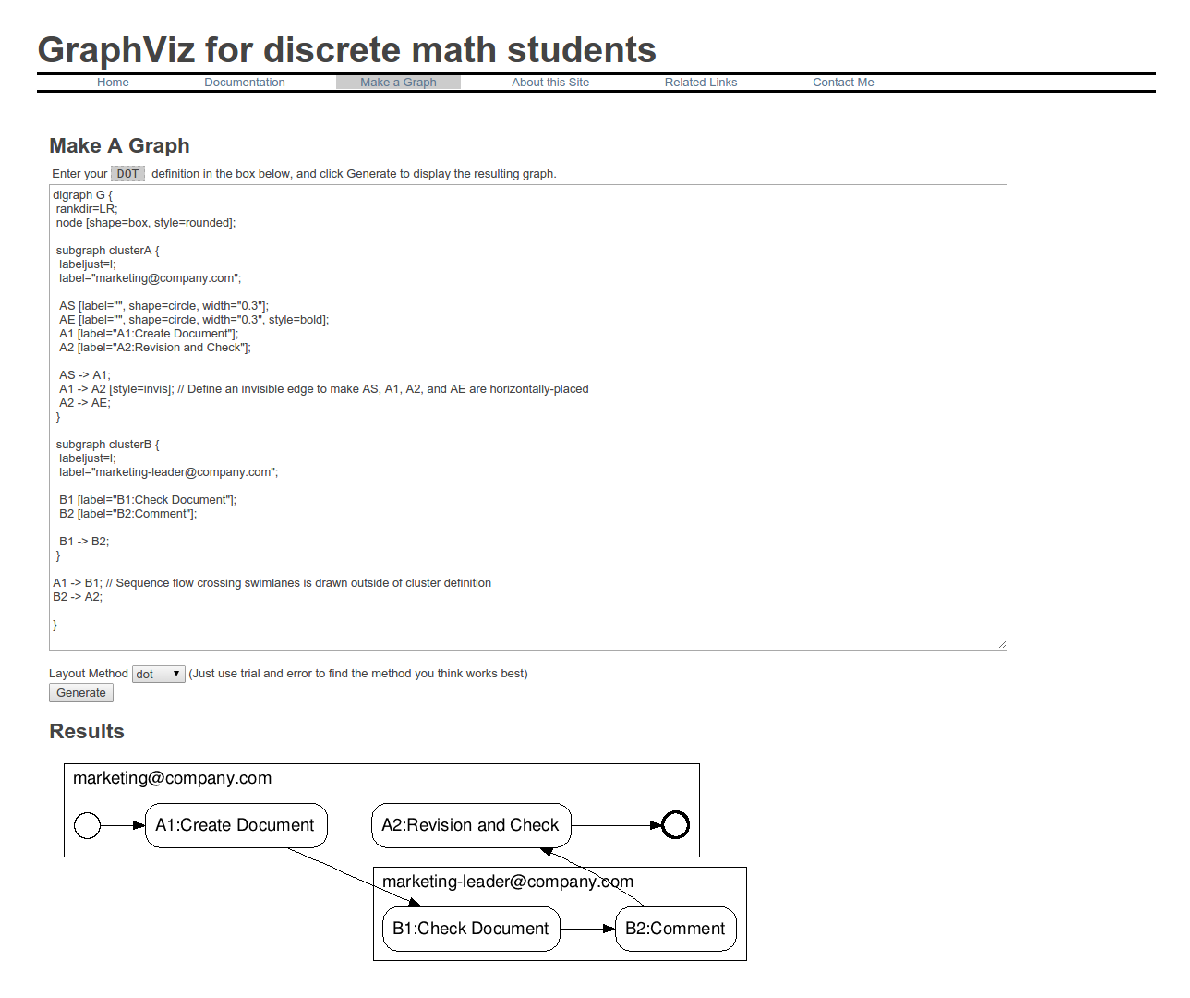
\includegraphics[width=1.0\textwidth]{img/dotfile.eps}
 \caption{Application Uses Dot File for Graph Generation}
 \label{fig:dotfile}
\end{figure}

\begin{figure}
 \centering
 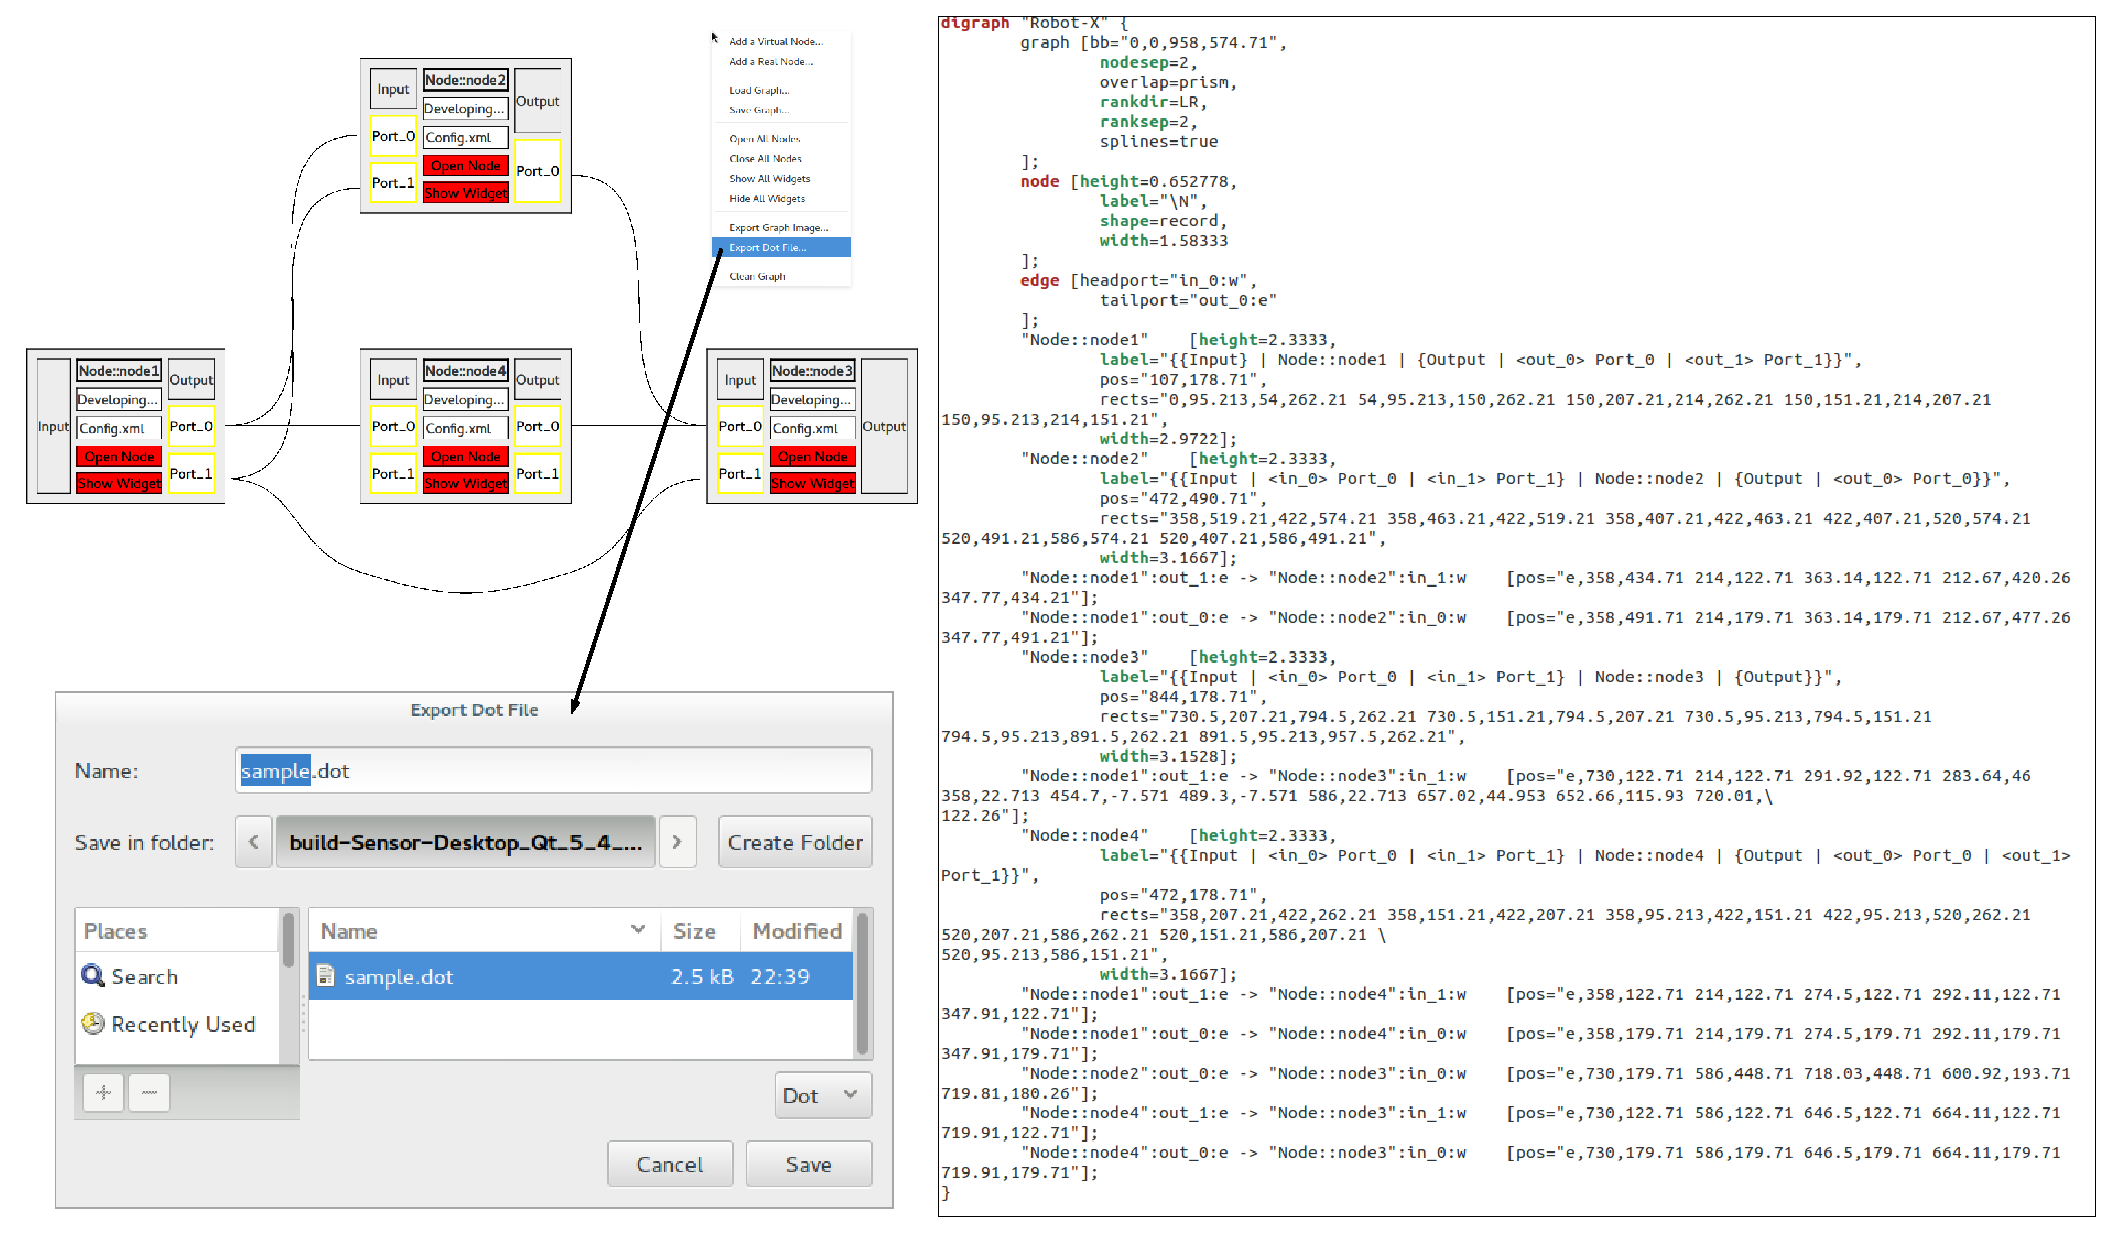
\includegraphics[width=1.0\textwidth]{img/exportdot.eps}
 \caption{Export Dot File of Abstract Graph Model and Its Contents}
 \label{fig:exportdot}
\end{figure}

\subsubsection{Zoom in and out}

If a graph is too large, the view port of Robot-X canvas will not have enough space to show entire graph. Robot-X provides a zoom in/out operation by using Ctrl + mouse wheel as shown in Fig.\ref{fig:zoom}.

\begin{figure}
 \centering
 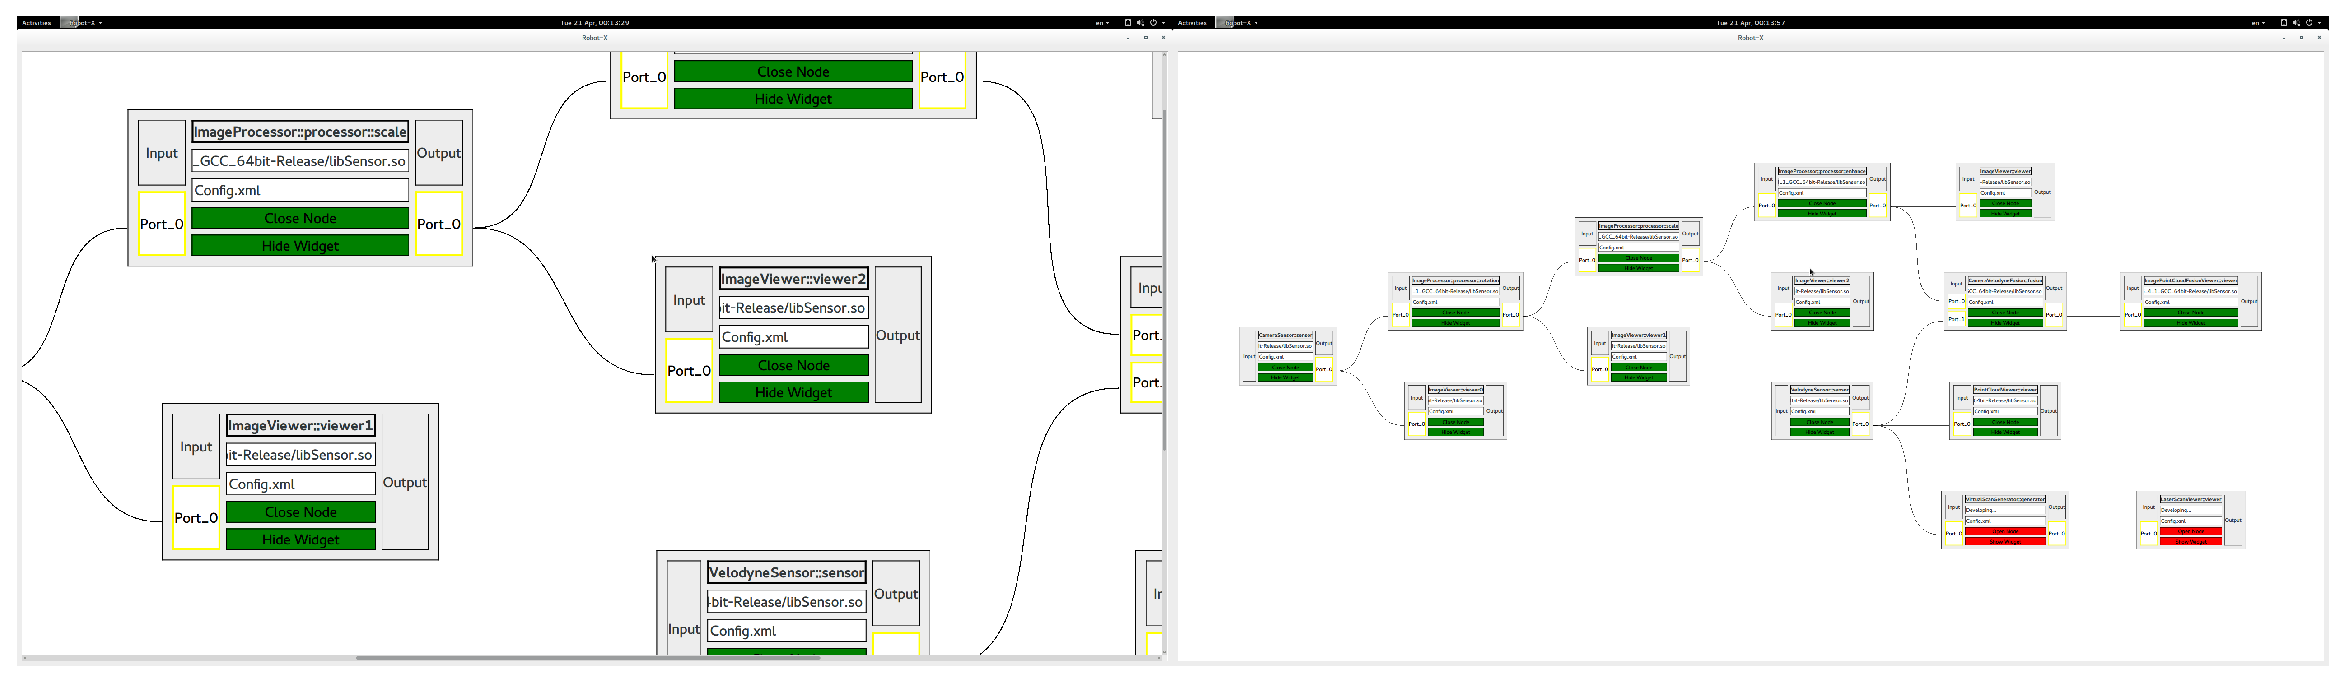
\includegraphics[width=1.0\textwidth]{img/zoom.eps}
 \caption{Zoom in and out of a Graph Model}
 \label{fig:zoom}
\end{figure}

\subsubsection{Clear Graph}

To clear graph, right click on empty part of Robot-X canvas and a menu pup up as shown in Fig.\ref{fig:cleargraph} left. After choosing "Clear Graph" all nodes and edges will be removed from graph model as well as functional modules and their communications as Fig.\ref{fig:cleargraph} right.

\begin{figure}
 \centering
 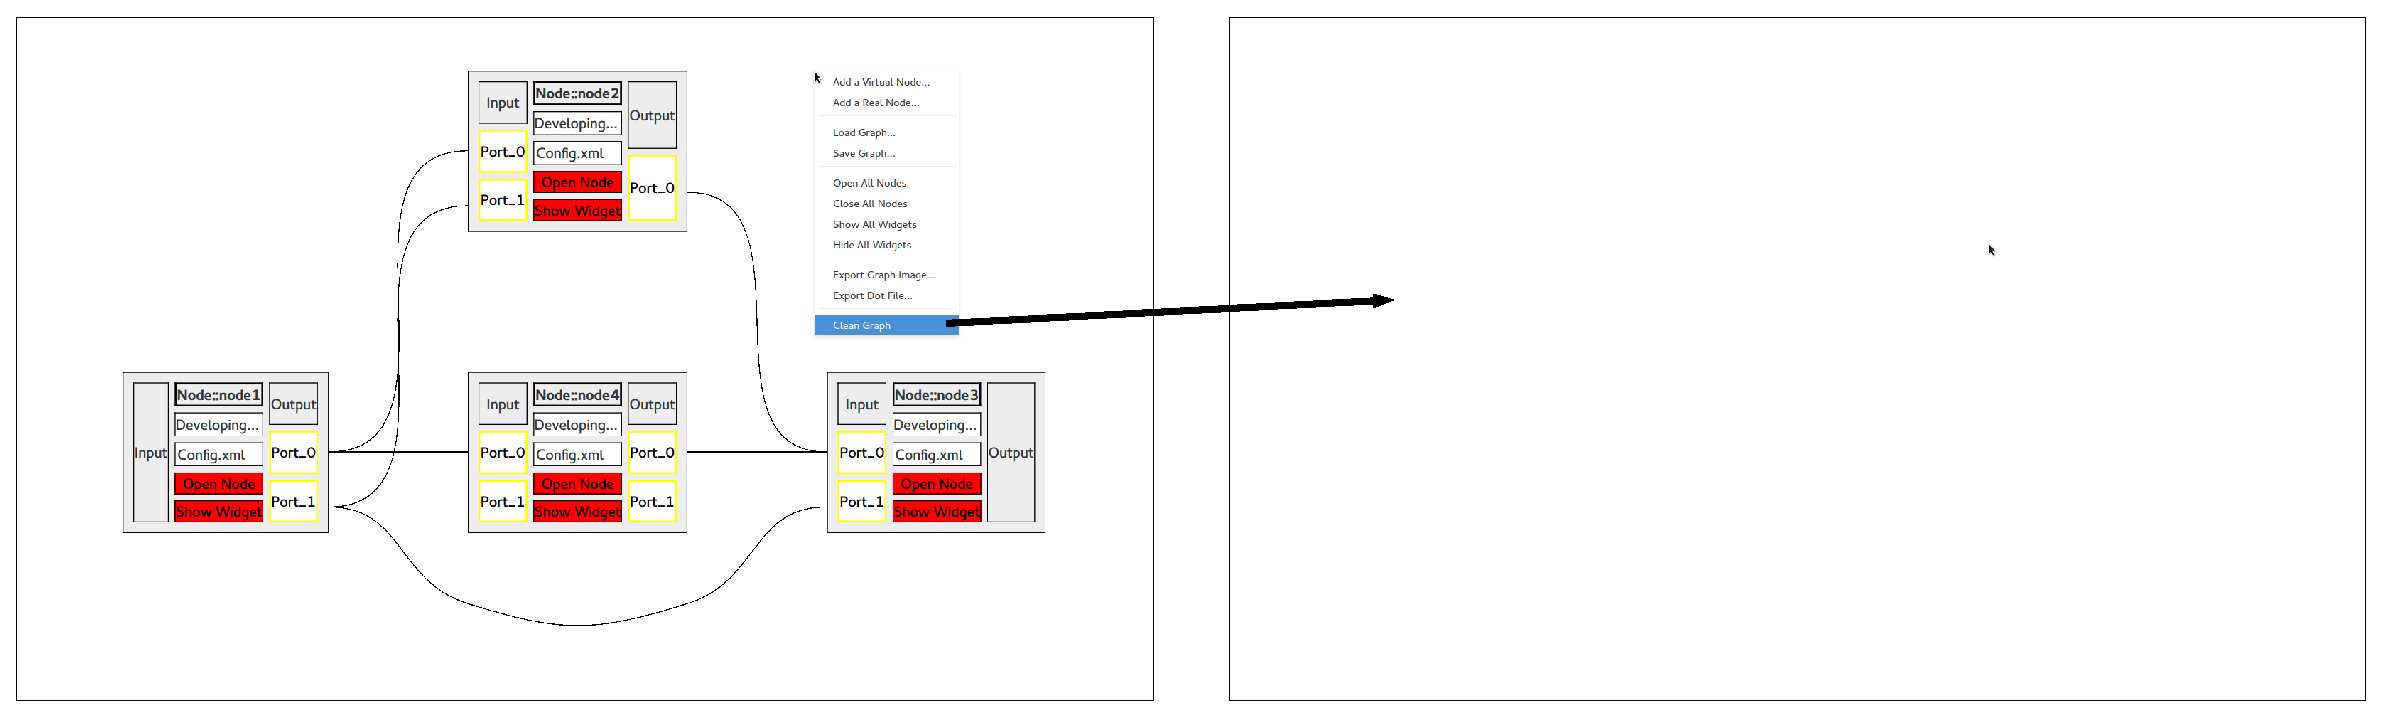
\includegraphics[width=1.0\textwidth]{img/cleargraph.eps}
 \caption{Clear an Abstract Graph Model}
 \label{fig:cleargraph}
\end{figure}

\section{Use Robot-X to Launch and Control Software}

After top abstract graph model construction and down functional modules development. Robot-X can launch software according to the concreted graph model (virtual nodes turn to real nodes), and fully control the software. Normally, the abstract graph model has been saved as graph file and it is not necessary to convert all virtual nodes to real nodes (sub-system of concreted sub-graph model could be launched as well).

\subsection{Open and Close Nodes}

You can use node's open/close button to control it as shown in Fig.\ref{fig:openclose}. The red color means the node is closed and you can open node by pushing this button. The green color means the node is open and you can close node by pushing this button. If a node is failed to open, the color will still be red and vise versa. Therefore, this could be regarded as an open/close status indicator of node.

\begin{figure}
 \centering
 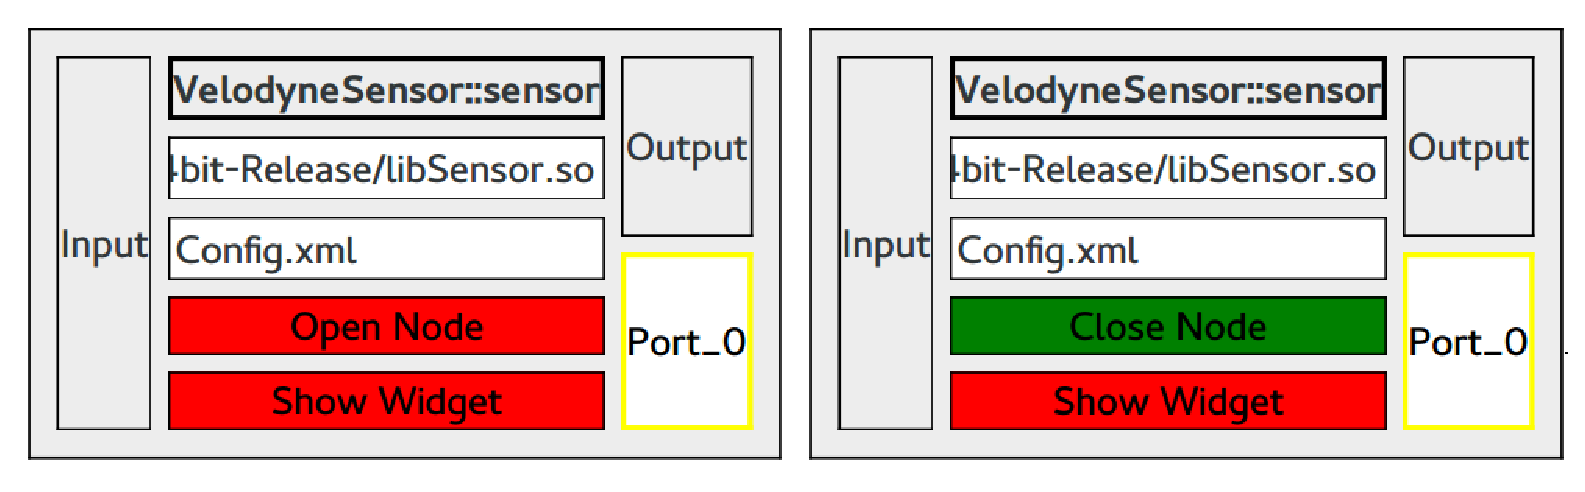
\includegraphics[width=0.6\textwidth]{img/openclose.eps}
 \caption{Open and Close a Node}
 \label{fig:openclose}
\end{figure}

Another convenient way is to use graph menu as shown in Fig.\ref{fig:openallnodes} top. Right click on empty part of Robot-X canvas, choose "Open All Nodes", then Robot-X will try to open all nodes. If successfully open a node, its open/close button will turn to green and if failed, its open/close button will keep in red as shown in Fig.\ref{fig:openallnodes} bottom. There are two virtual nodes in this example, therefore, after opening all nodes operation, they are still in red color. For closing all nodes operation, it is same with that of opening all nodes.

\begin{figure}
 \centering
 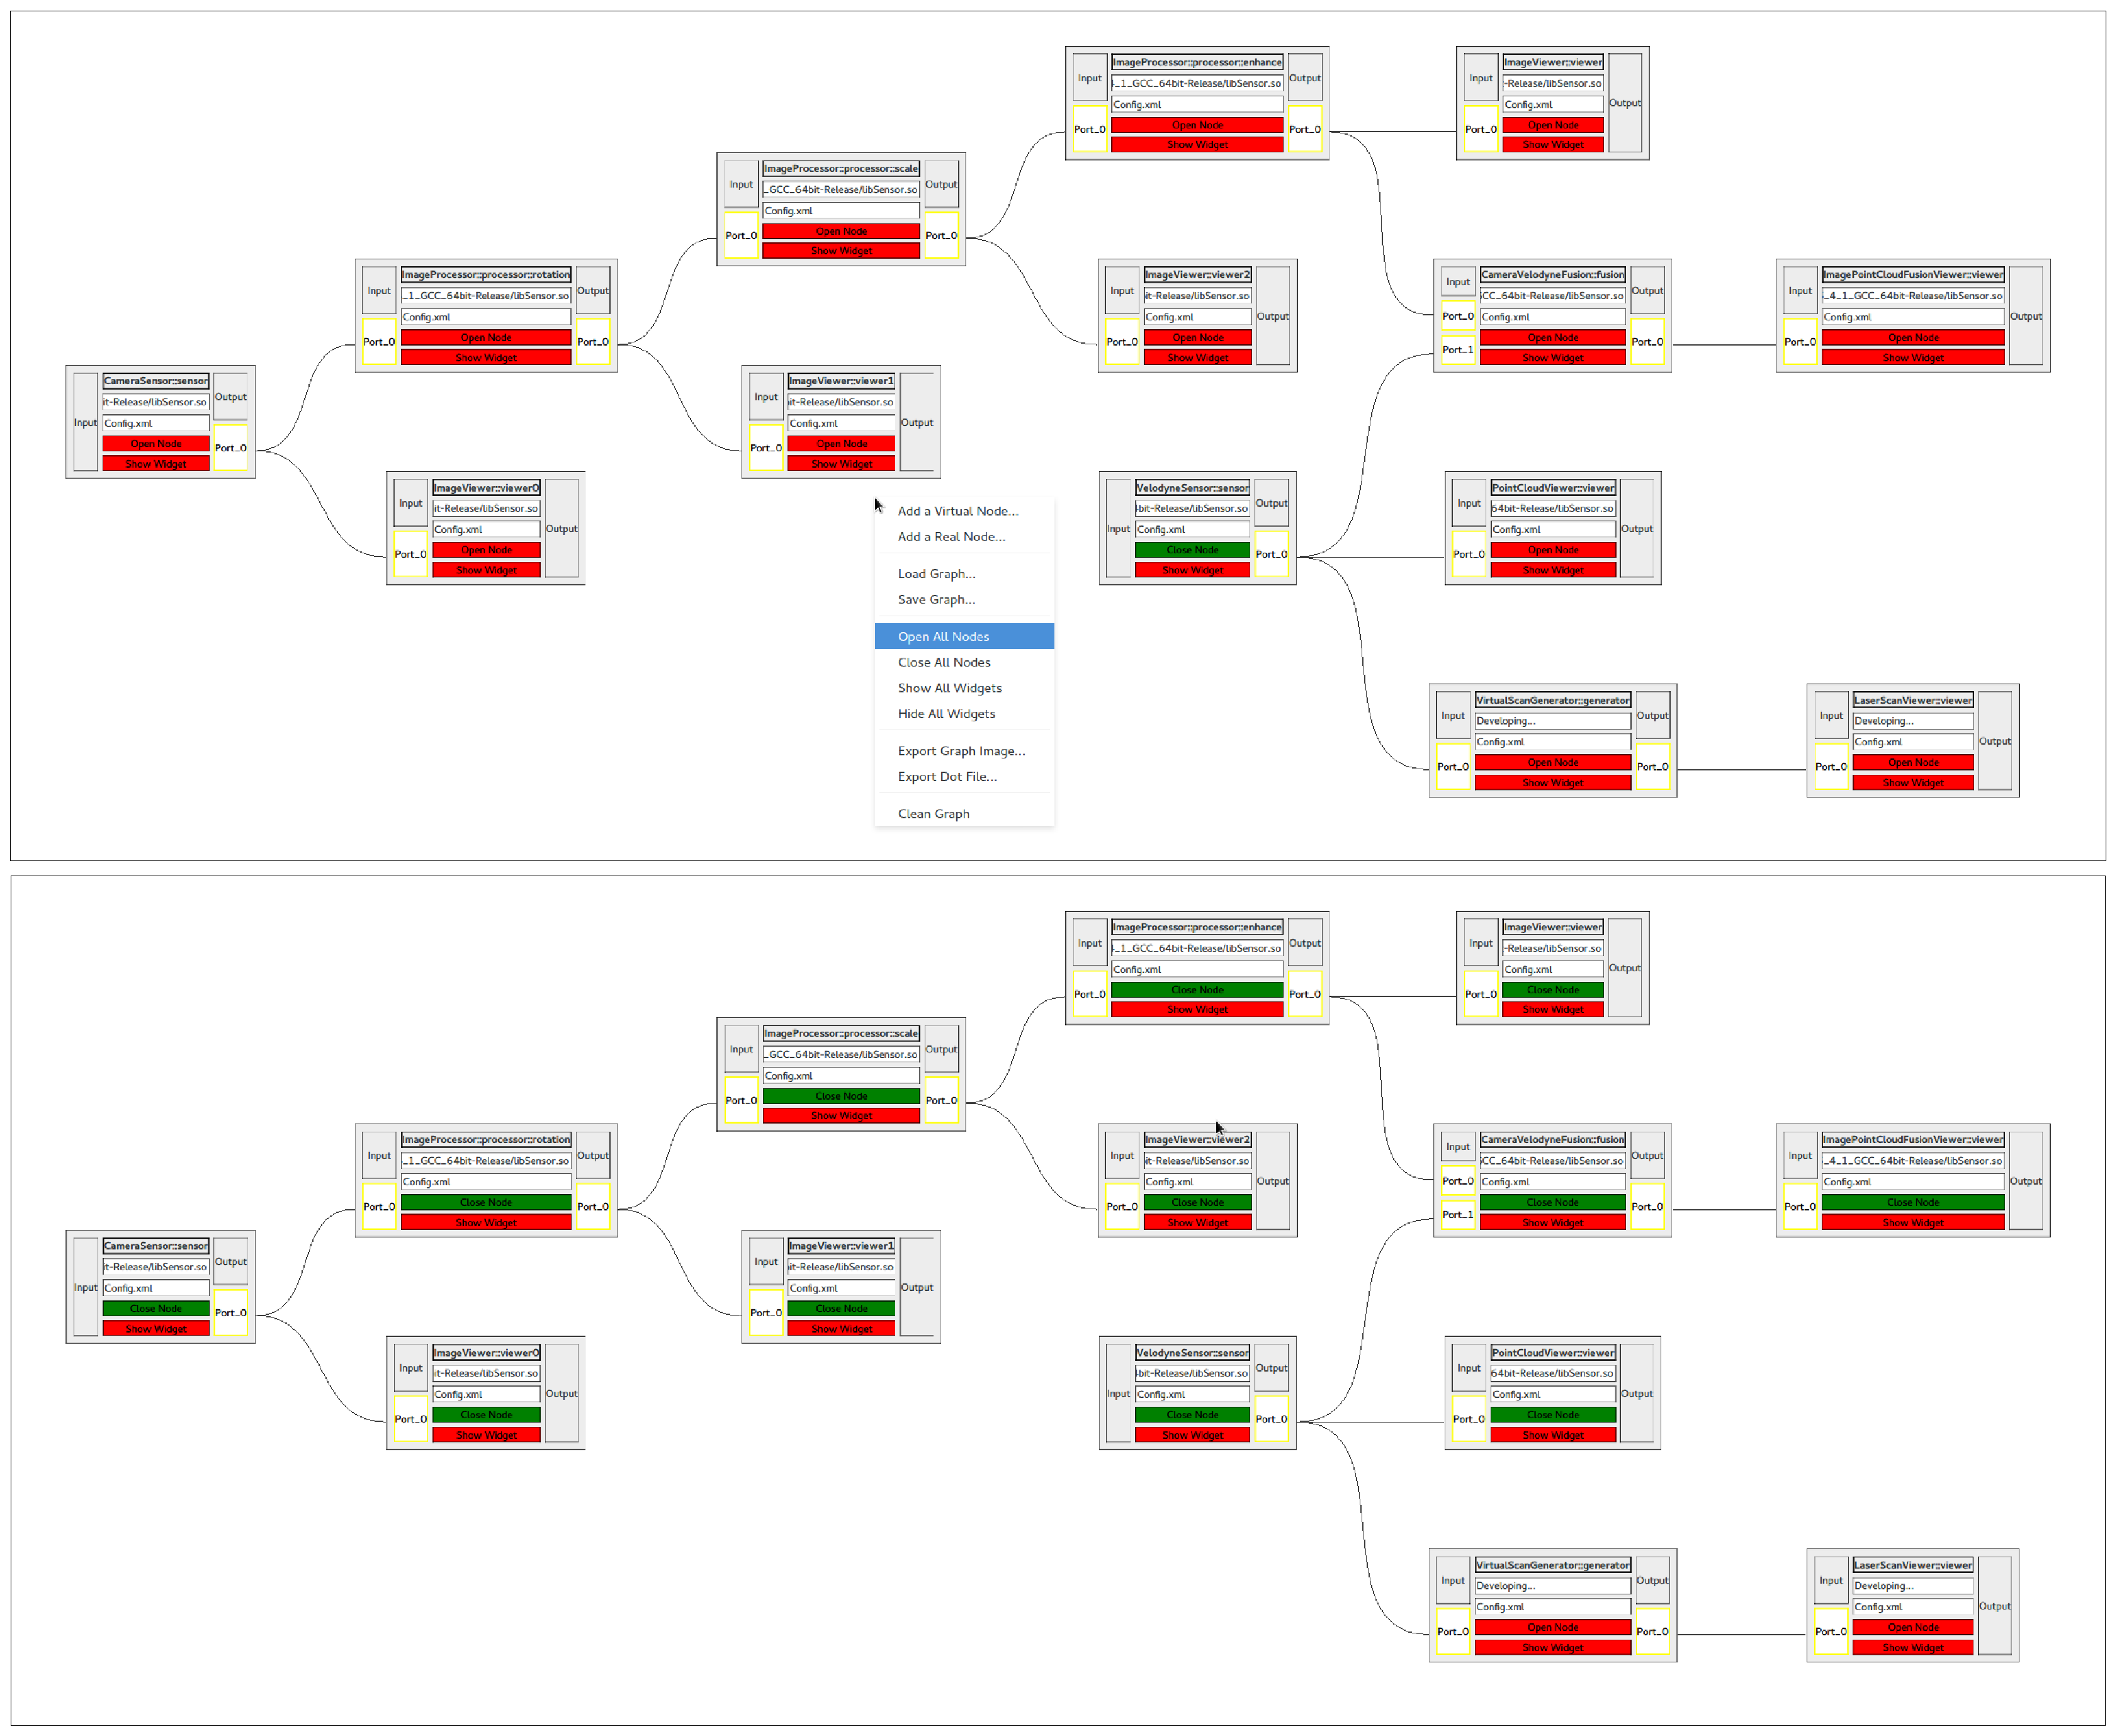
\includegraphics[width=0.9\textwidth]{img/openallnodes.eps}
 \caption{Open All Nodes}
 \label{fig:openallnodes}
\end{figure}

\subsection{Show and Hide Widgets}

Widget is a GUI to show something on the screen. RobotSDK 4.0 provides a uniform way to program such widget (see Chapter \ref{module}). Similar to open/close nodes, to show/hide widgets could be conducted by pushing each node's show/hide widget button as shown in Fig.\ref{fig:showhidewidget} and also by using graph menu as shown in Fig.\ref{fig:showallwidgets}. The widgets of this example is shown as Fig.\ref{fig:allwidgets}.

There is one thing need to be noticed. If a node has widget and the node also wants to control this widget, then it must be in the GUI thread, which is also the thread of application (For example, Robot-X). For a non-GUI node without showing widget, if you push show widget button, it will also turn to green, however, no widget will appear. Because unlike open/close operation, show/hide operation does not check widget status but only sends a command. Therefore, if you manually close a widget by pressing its top-right cross button, the show/hide button will not turn to red. Fortunately, this will not cause crash and you can still use show widget button to show the closed widget again.

\begin{figure}
 \centering
 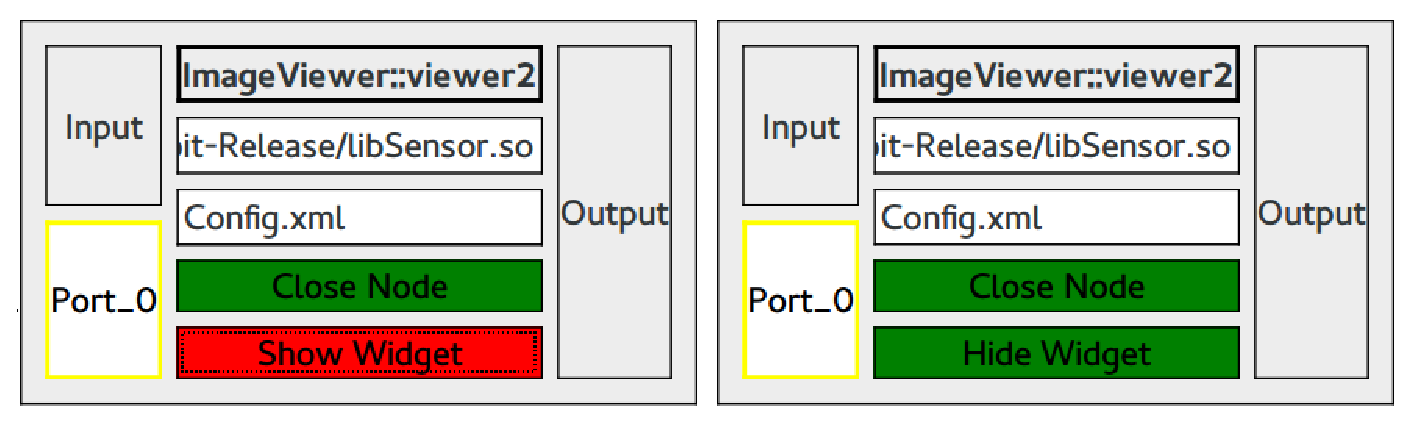
\includegraphics[width=0.6\textwidth]{img/showhidewidget.eps}
 \caption{Show and Hide Widget}
 \label{fig:showhidewidget}
\end{figure}

\begin{figure}
 \centering
 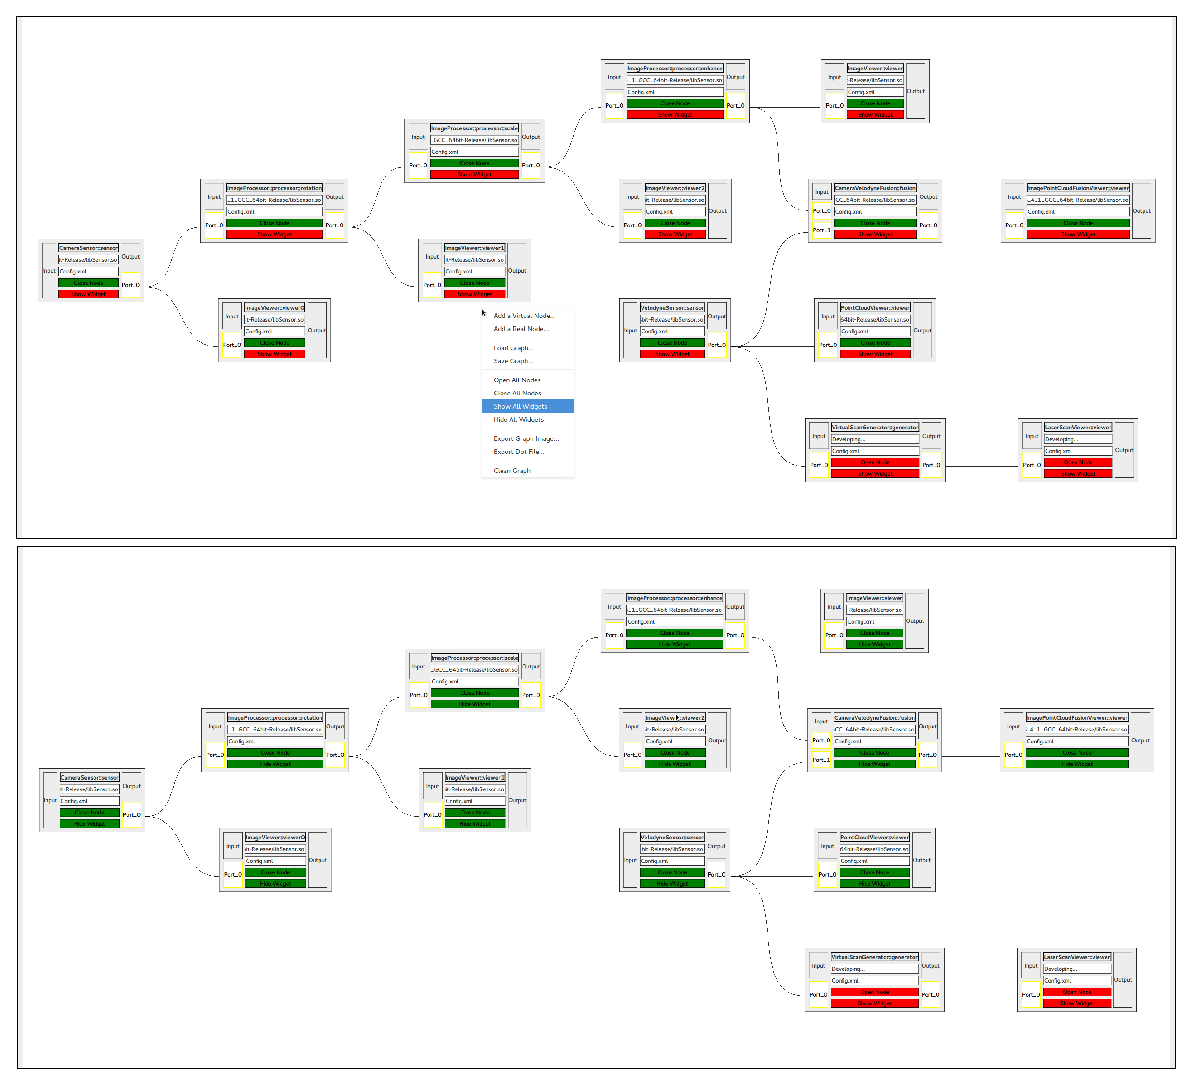
\includegraphics[width=0.9\textwidth]{img/showallwidgets.eps}
 \caption{Show All Widgets}
 \label{fig:showallwidgets}
\end{figure}

\begin{figure}
 \centering
 \includegraphics[width=1.0\textwidth]{img/allwidgets.eps}
 \caption{Widgets of the Example: Fusion of Camera and Velodyne}
 \label{fig:allwidgets}
\end{figure}

\chapter{Functional Module Development: Free C Style Programming} \label{module}

Robot-X is a super high level application, therefore, from RobotSDK 4.0, users need not to develop high level applications and could focus on functional modules development. In this chapter, we will present basic but enough instructions for common functional module development. We strongly recommend developers to use QtCreator as IDE for functional module development, however, we will still briefly introduce how to use Visual Studio for such development in Windows just after presenting that with QtCreator.

\section{Project Configuration}

\subsection{Create Shared Library Project}

The functional modules are packed in shared library, therefore, we should first build a shared library project. After starting QtCreator, click "New Project",  and then choose "Library" and "C++ Library" as Fig.\ref{fig:newproject1}. Then a series of configuration dialog will appear as Fig.\ref{fig:newproject2} and you only need to to make sure that the "Library Type" should be "Shard Library" in the first dialog. Then you will get a "shared library project" as Fig.\ref{fig:newproject2} bottom-right. You can freely delete the auto-generated .h and .cpp files as you wish, because they are useless and will not affect functional modules.

\begin{figure}
 \centering
 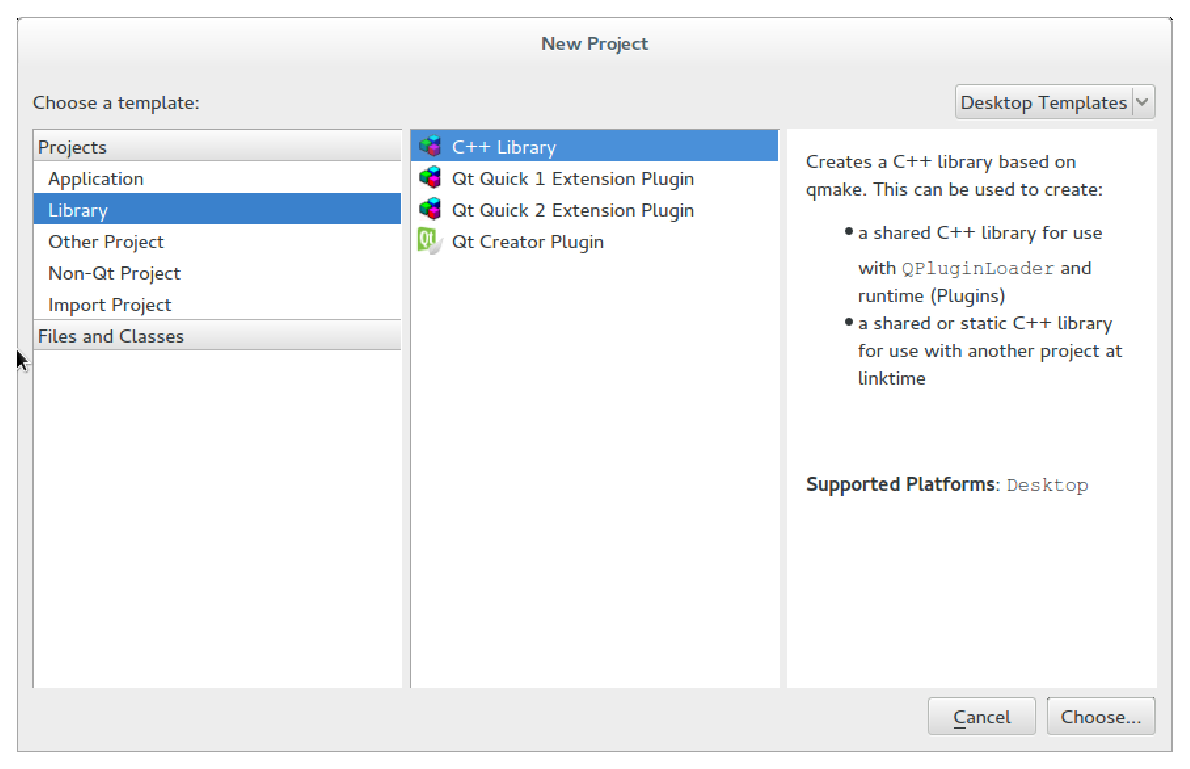
\includegraphics[width=0.6\textwidth]{img/newproject1.eps}
 \caption{Create a C++ Library Project}
 \label{fig:newproject1}
\end{figure}

\begin{figure}
 \centering
 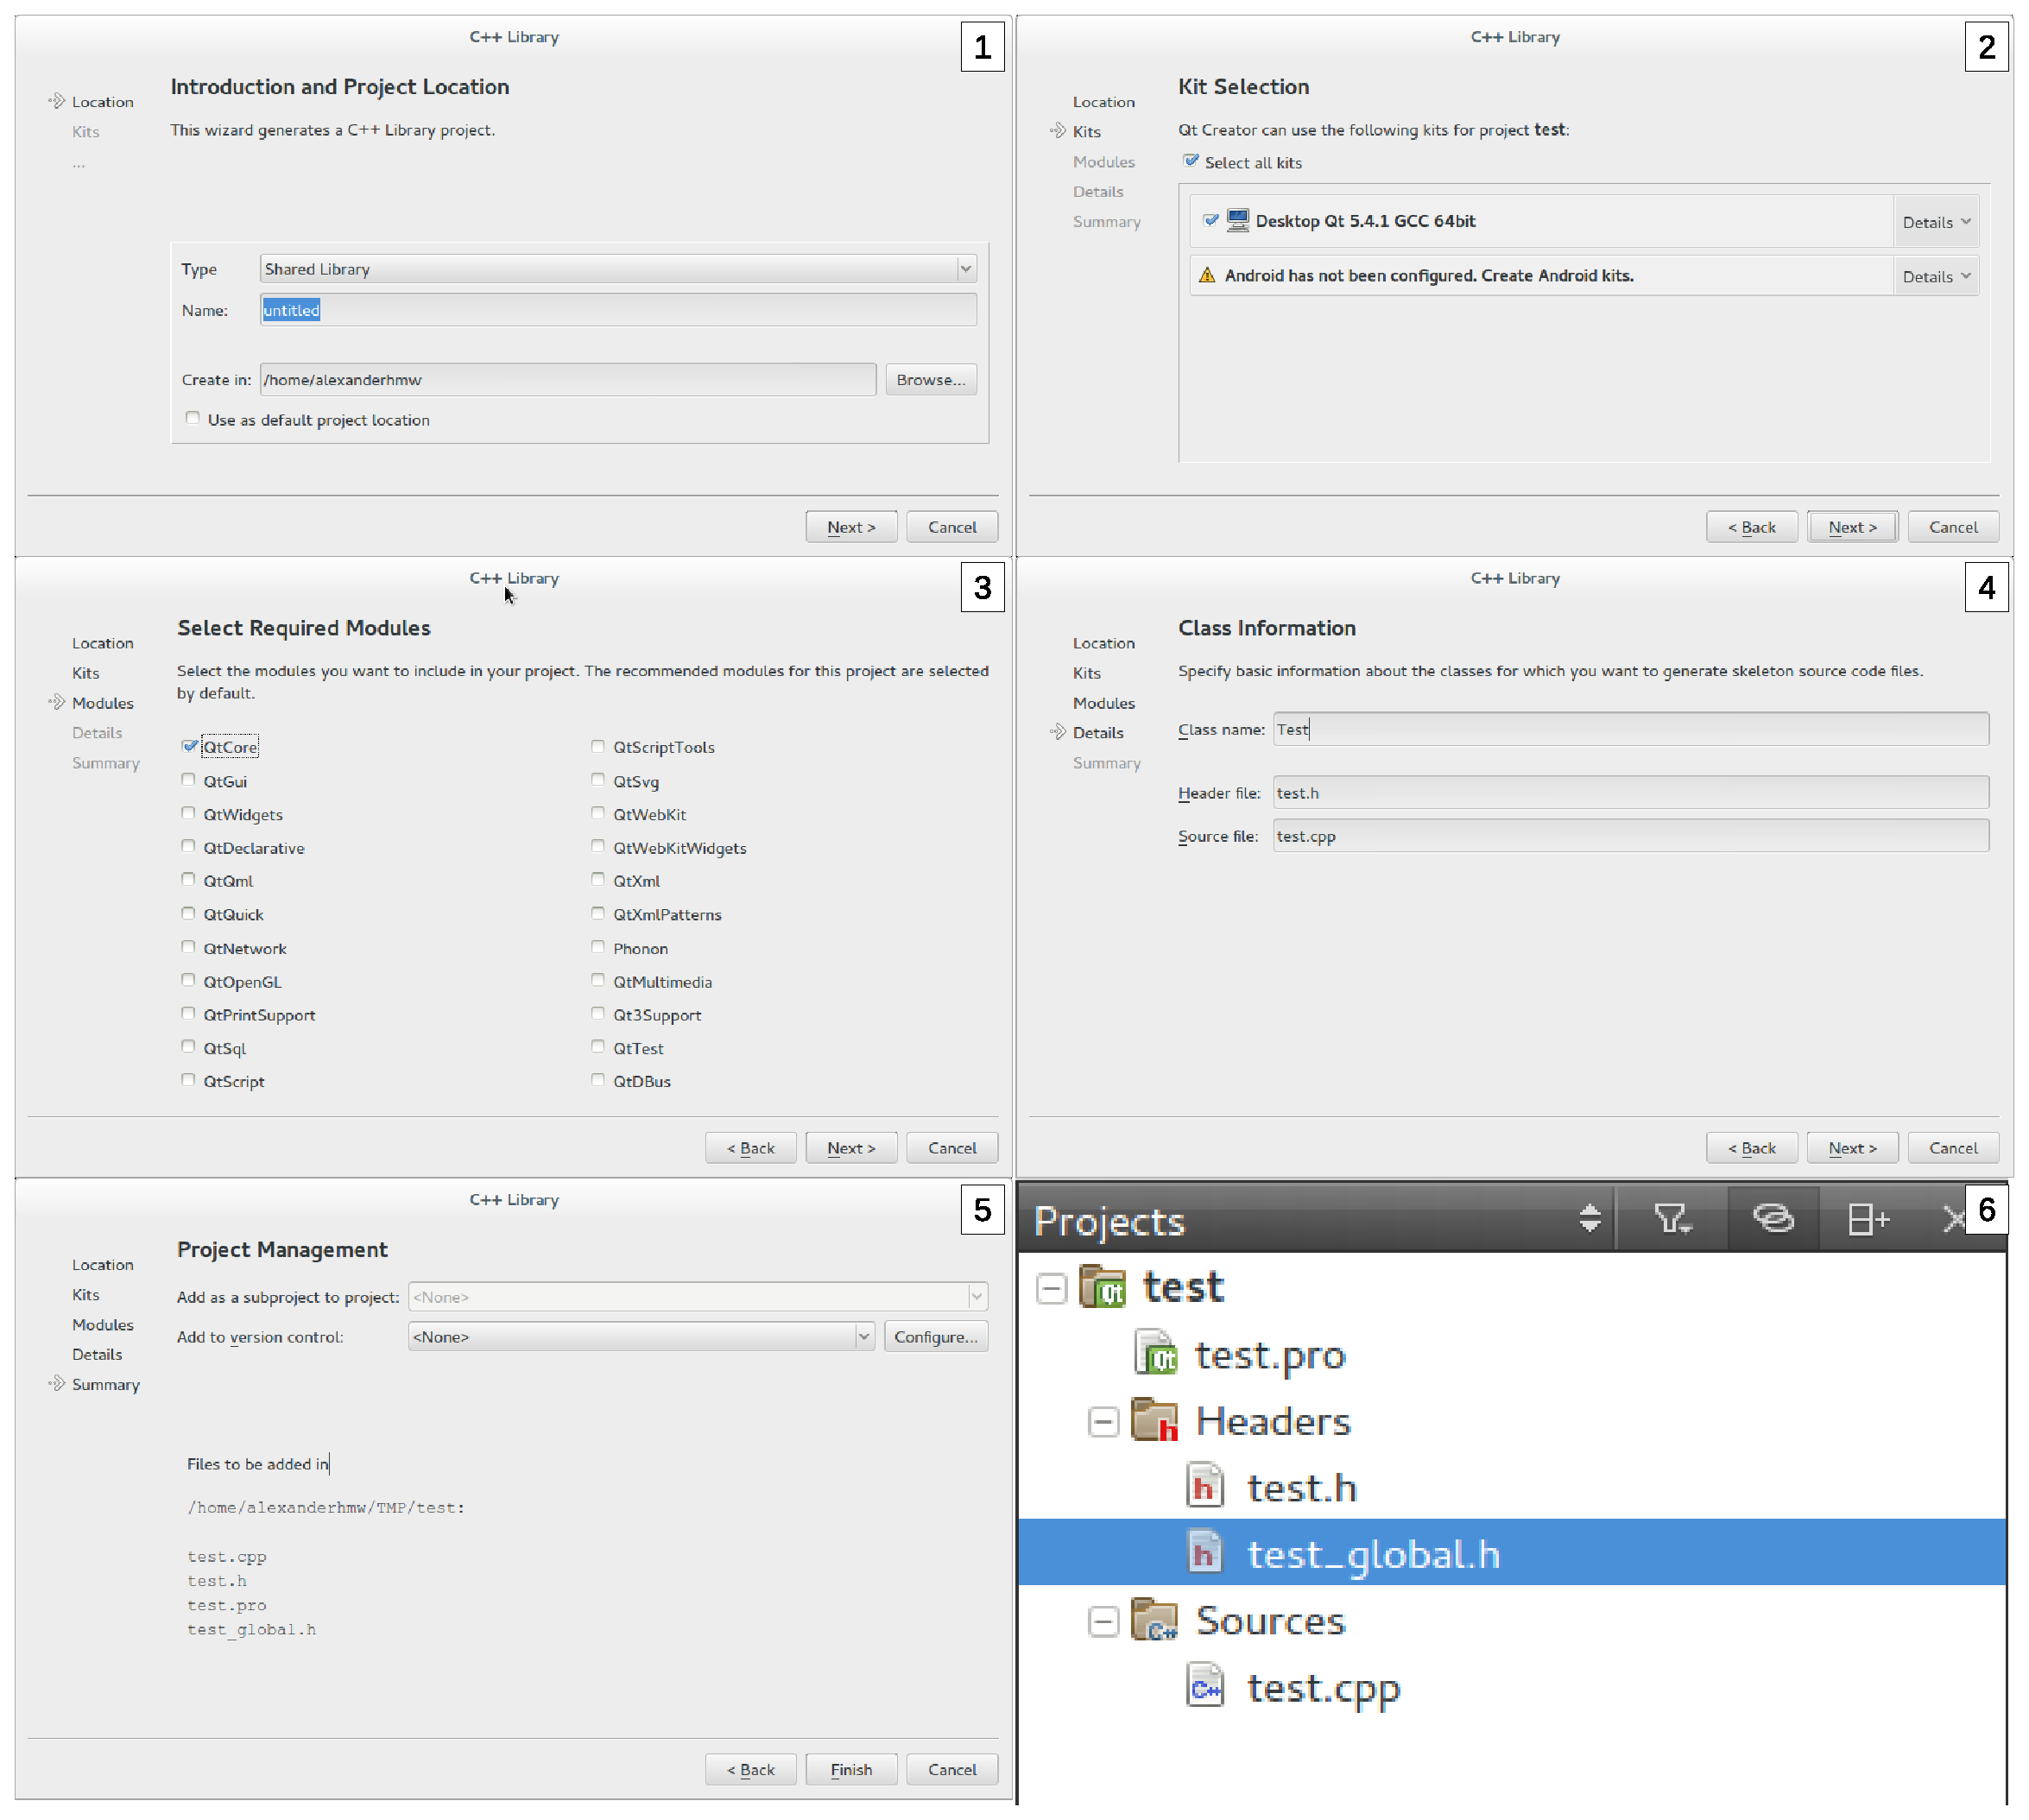
\includegraphics[width=0.6\textwidth]{img/newproject2.eps}
 \caption{Configure a C++ Library Project}
 \label{fig:newproject2}
\end{figure}

\subsection{Configure Project with RobotSDK}

After creating shared library project, we need to configure this project with RobotSDK. Open the .pro file in the project panel as Fig.\ref{fig:newproject2} bottom-right and we will see its contents as Fig.\ref{fig:configproject1} top-left. Remember to add build step with argument install. The only thing you need to do is to include "RobotSDK.pri" file as Fig.\ref{fig:configproject1} right (you need to choose one according to your OS), or you can just include \\(\$\$(ROBOTSDKMODULE)) which is a new added macro. The configuration is done.

[Update-150427] You can use "MODULES" in front the "include" sentence to include other module's header file. See "Module" in source code. 

If you intend to use QtCreator to build and deploy modules, please remember to add a build step with argument install in Project Configuration Panel. 

\begin{figure}
 \centering
 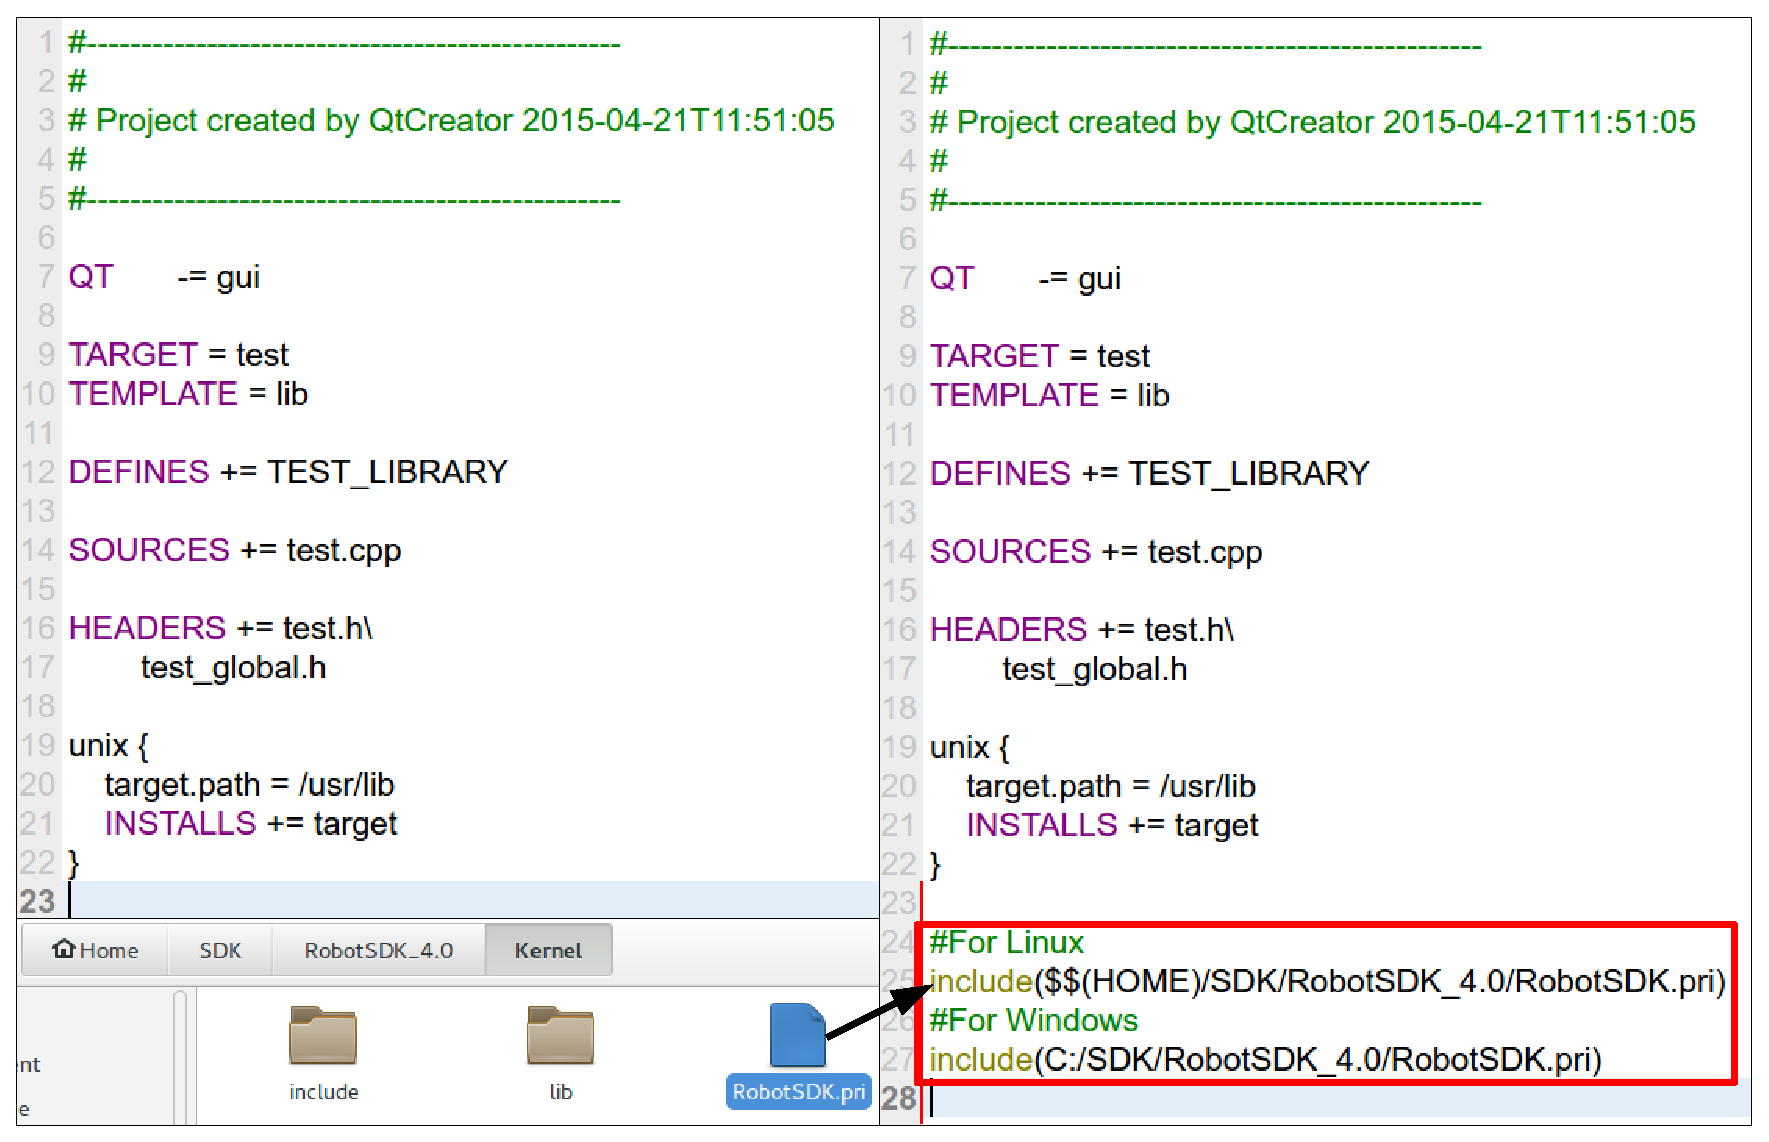
\includegraphics[width=0.6\textwidth]{img/configproject1.eps}
 \caption{Configure a C++ Library Project}
 \label{fig:configproject1}
\end{figure}

\subsection{For Visual Studio}

For Visual Studio, you need to create a dynamic link library (dll) project via Qt Visual Studio Add-in. Then you can regard RobotSDK as a library and add its include path and static libraries "Kernel\_Debug.lib" or "Kernel\_Release.lib" (Fig.\ref{fig:configproject1} bottom-left) to the VS project. You also need to add Eigen include path if you want to use GLViewer or Kernel is already compiled with GLViewer.

\section{Basic Steps to Program Functional Module}

From Chapter \ref{robotx}, we know that the Robot-X will generate two files for each functional module. Then you need to add them to the created shared library project. In this section we will separately introduce how to program these files.

\subsection{Header File}

\subsubsection{Step 1: Add Required Headers [C Style]}

Just like C programming, you need to refer other headers for programming as Fig.\ref{fig:header1}. Normally, you need to add other module's header as required input node and library headers, like "OpenCV", "PCL", etc. Here we stress the position of headers as below.

\begin{framed}
 Included headers must be in front of Node Configuration (see following section)
\end{framed}

\begin{figure}
 \centering
 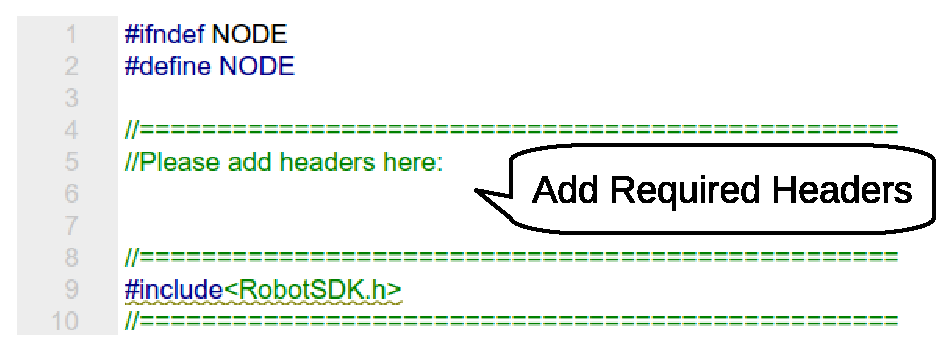
\includegraphics[width=0.4\textwidth]{img/header1.eps}
 \caption{Add Required Headers}
 \label{fig:header1}
\end{figure}

\subsubsection{Step 2: Configure Node}

As shown in Fig.\ref{fig:header2}, The "Node Class", "Input Port Number" and "Output Port Number" have already been automatically set. If the node has input ports, a segment of commented codes will appear as Fig.\ref{fig:header2} bottom. You need to uncomment these codes and fill in the "Input Node Class Name". If you forget this, you cannot access input "Params" and "Data" via RobotSDK. 

[Update-150427] The PORT\_DECL has been moved to cpp file for port toolkit.

\begin{figure}
 \centering
 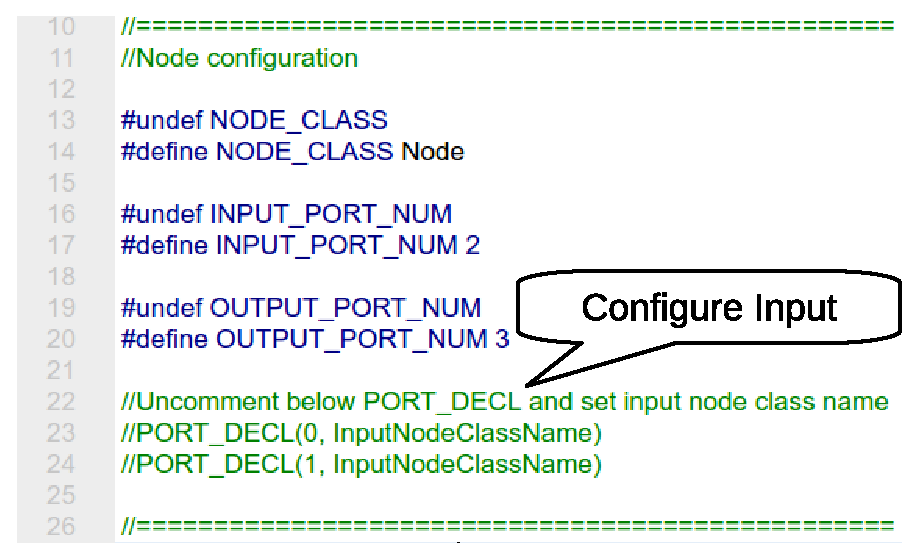
\includegraphics[width=0.4\textwidth]{img/header2.eps}
 \caption{Configure Node}
 \label{fig:header2}
\end{figure}

\subsubsection{Step 3: Add Elements to "Params", "Vars" and "Data"}

Similar to RobotSDK 3.0, a node contains a public "Params" and a private "Vars", and outputs "Data" frame by frame. You still need to add elements for them. However, thanks to C++11 techniques listed below, a set of syntax is created for convenient adding and managing elements. We will present how to add elements in section \ref{syntax}.

\begin{itemize}
 \item Non-static data members initializers \\
 \url{http://en.cppreference.com/w/cpp/language/data_members}
 \item Lambda function \\
 \url{http://en.cppreference.com/w/cpp/language/lambda}
 \item Variadic Macro \\
 \url{http://en.wikipedia.org/wiki/Variadic_macro}
\end{itemize}

\begin{figure}
 \centering
 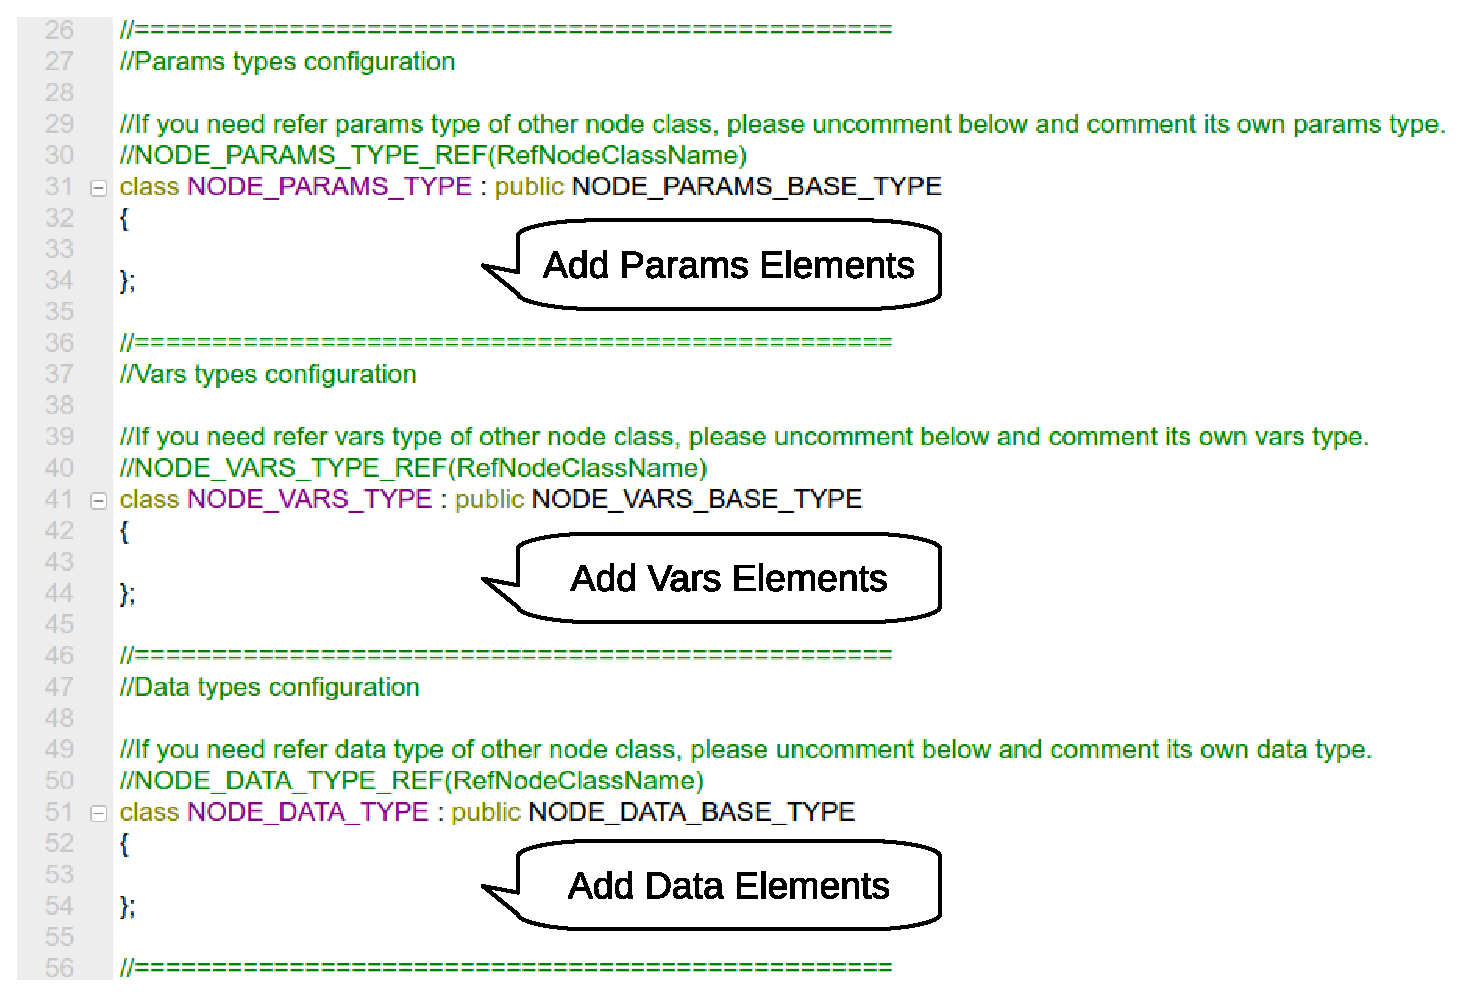
\includegraphics[width=0.6\textwidth]{img/header3.eps}
 \caption{Add Elements to "Params", "Vars" and "Data"}
 \label{fig:header3}
\end{figure}

\subsubsection{Step 4: Declare functions [C Style]} \label{declfunc}

Just like C programming, sometimes, you need to declare functions first in the header file as in Fig.\ref{fig:header4}. There are two types of declaration: 1) original C style function declaration and 2) wrapped function declaration by RobotSDK syntax. The only difference between them is the former one cannot directly access node's "Params", "Vars", "Data" and input nodes' "Params", "Data" ({\bf{Ordinary Function}}), and the latter one can directly access them via RobotSDK syntax ({\bf{Node Function}}). We will present how to declare such function in section \ref{syntax}.

\begin{figure}
 \centering
 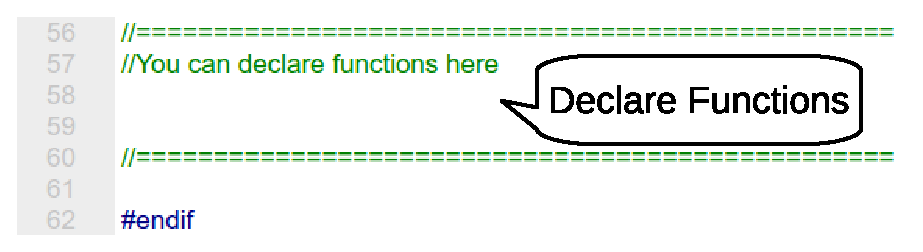
\includegraphics[width=0.4\textwidth]{img/header4.eps}
 \caption{Declare Functions}
 \label{fig:header4}
\end{figure}

\subsection{Source File}

\subsubsection{Step 1: Choose Node}

RobotSDK 4.0 uniformed all node types used in RobotSDK 3.0 and this enables Robot-X to be a super high level application. However, it is still free for developers to extend the default node and use extended node in module programming. As shown in Fig.\ref{fig:source1}, the default node is used automatically. If you want to use extended node, you just need to replace the "USE\_DEFAULT\_NODE" with "USE\_EXTENDED\_NODE(ExtendedNodeClass[,...])". We will discuss the extended node in Chapter \ref{nodeextension}.

\begin{framed}
 Here, the "NodeClass" is different with the module's "Node Class". The former one is a real class inherited from "Node" class in Kernel and the latter one is only an identifier for the module.
\end{framed}

\begin{figure}
 \centering
 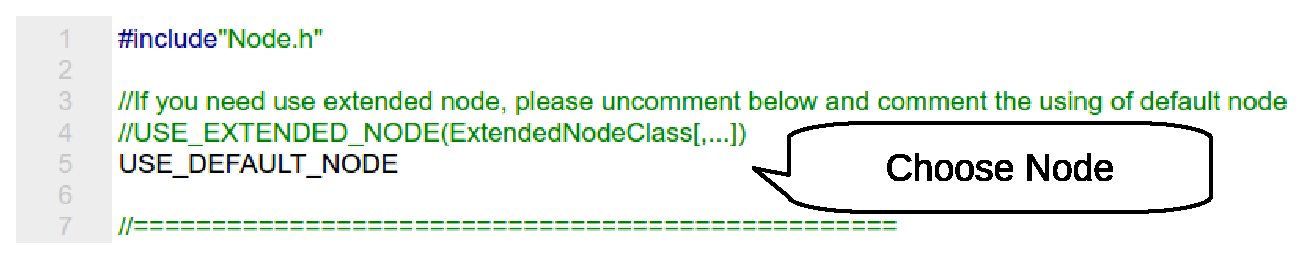
\includegraphics[width=0.6\textwidth]{img/source1.eps}
 \caption{Choose Node}
 \label{fig:source1}
\end{figure}

\subsubsection{Step 2: Functions Programming [C Style]}

Now, you are free to program module's functions. From section \ref{declfunc}, we know there are two types of function: 1) Ordinary Function and 2) Node Function. Here we stress them again and show details of Node Function in section \ref{syntax}.

\begin{framed}
 \begin{itemize}
  \item {\bf{Ordinary Function}}: original C style function which cannot directly access node's "Params", "Vars", "Data" and input nodes' "Params", "Data"
  \item {\bf{Node Function}}: wrapped function by RobotSDK syntax which can directly access them
 \end{itemize}
\end{framed}

As shown in Fig.\ref{fig:source2}, there are 4 default Node Functions: "initializeNode", "openNode", "closeNode" and "main" and their return value type are boolean. From the comments, only the "main" Node Function is mandatory and similar to C programming, it is the main entry of the module (you should not replace it with Ordinary Function). However, it is not the only main entry for the module, because, you can freely add main entries by extending default node (see Chapter \ref{nodeextension}). The correspondences between these four default functions and node's state is shown as Fig.\ref{fig:code}.

\begin{figure}
 \centering
 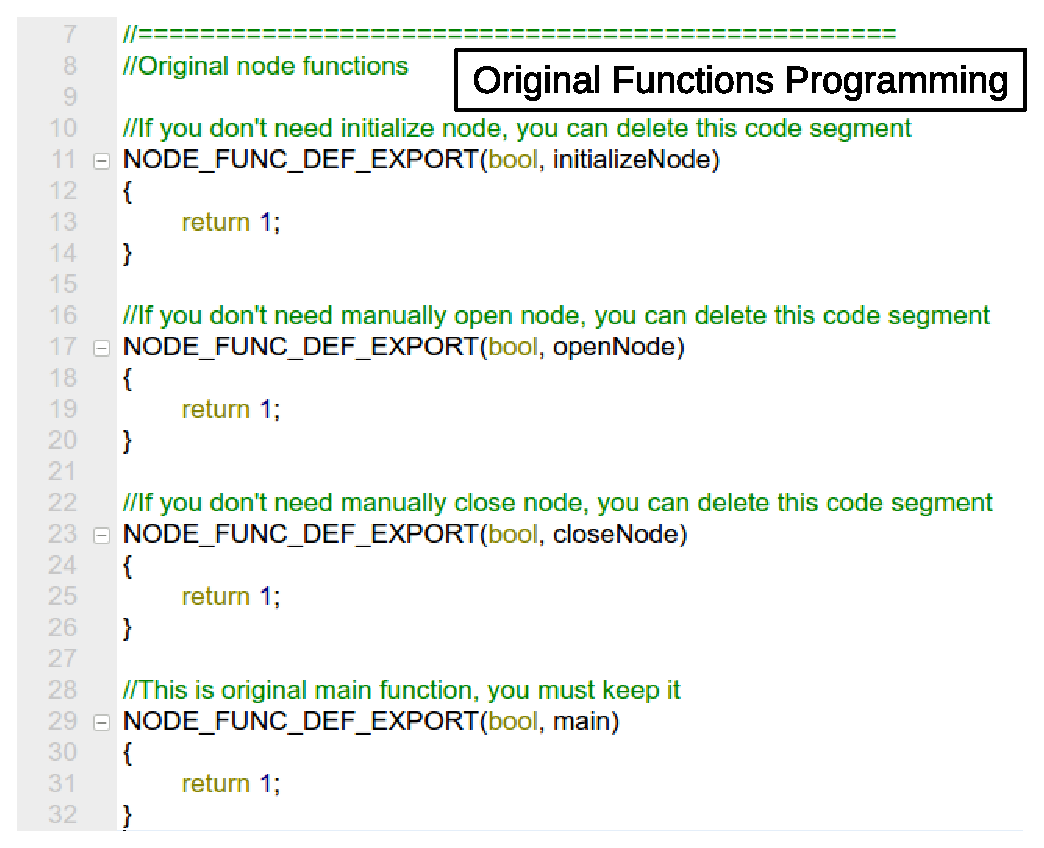
\includegraphics[width=0.5\textwidth]{img/source2.eps}
 \caption{Original Functions}
 \label{fig:source2}
\end{figure}

You can define your own Ordinary Functions and Node Functions as you want. But here we must stress the function call rule for them below and we will discuss the conversion between Ordinary Function and Node Function in section \ref{syntax}.

\begin{framed}
 \begin{itemize}
  \item Ordinary Function can call Ordinary Function via original C way.
  \item Ordinary Function cannot call Node Function.
  \item Node Function can call Ordinary Function via original C way.
  \item Node Function can call Node Function via RobotSDK syntax.
 \end{itemize}
\end{framed}

Another thing is about the extension of module. As Fig.\ref{fig:source3}, we create a node with extension and generate its code as Fig.\ref{fig:source4}. You can find that Robot-X appends the extension code to the source file. Therefore, we say that module extension shares the node configuration, value types and some functions with the base module. If you only generate code for module extension, Robot-X will first generate code of base module and then append code of extension. From the comments, all the 4 default functions are not mandatory. Here we need to inform users a controversial rule as below.

\begin{framed}
 During node construction, if the node requires an extended Node Function, the Kernel will first locates it with "Node Class" and "ExName". If not found, the Kernel will try to locates its original Node Function with "Node Class" for instead. If not found again, the node construction failed. 
\end{framed}

\begin{figure}
 \centering
 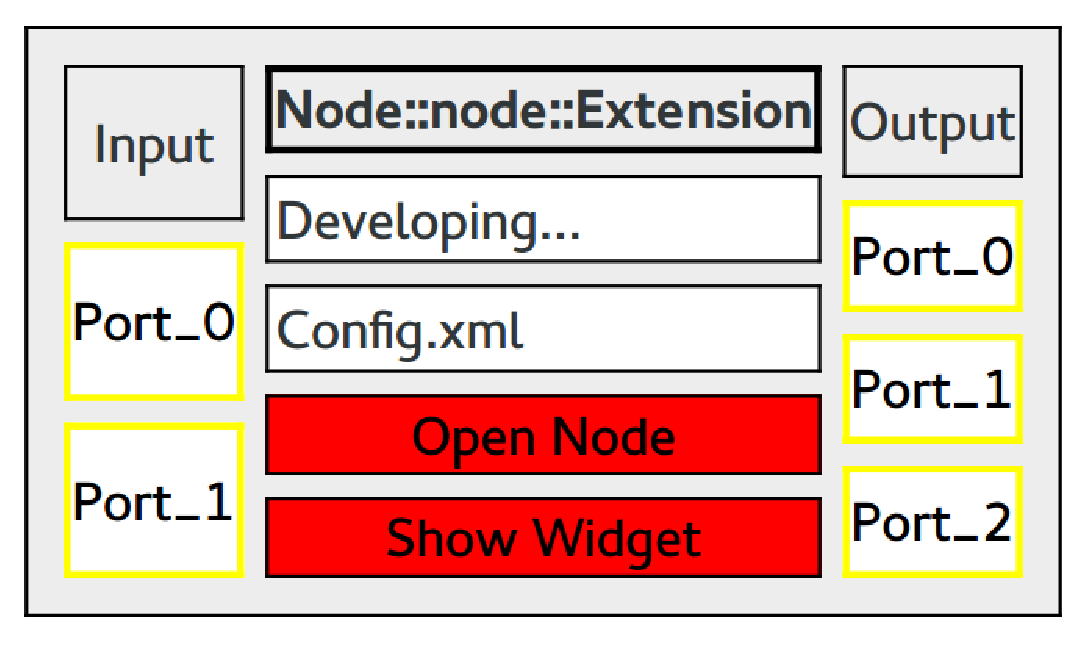
\includegraphics[width=0.3\textwidth]{img/source3.eps}
 \caption{Node with Extension}
 \label{fig:source3}
\end{figure}



\begin{figure}
 \centering
 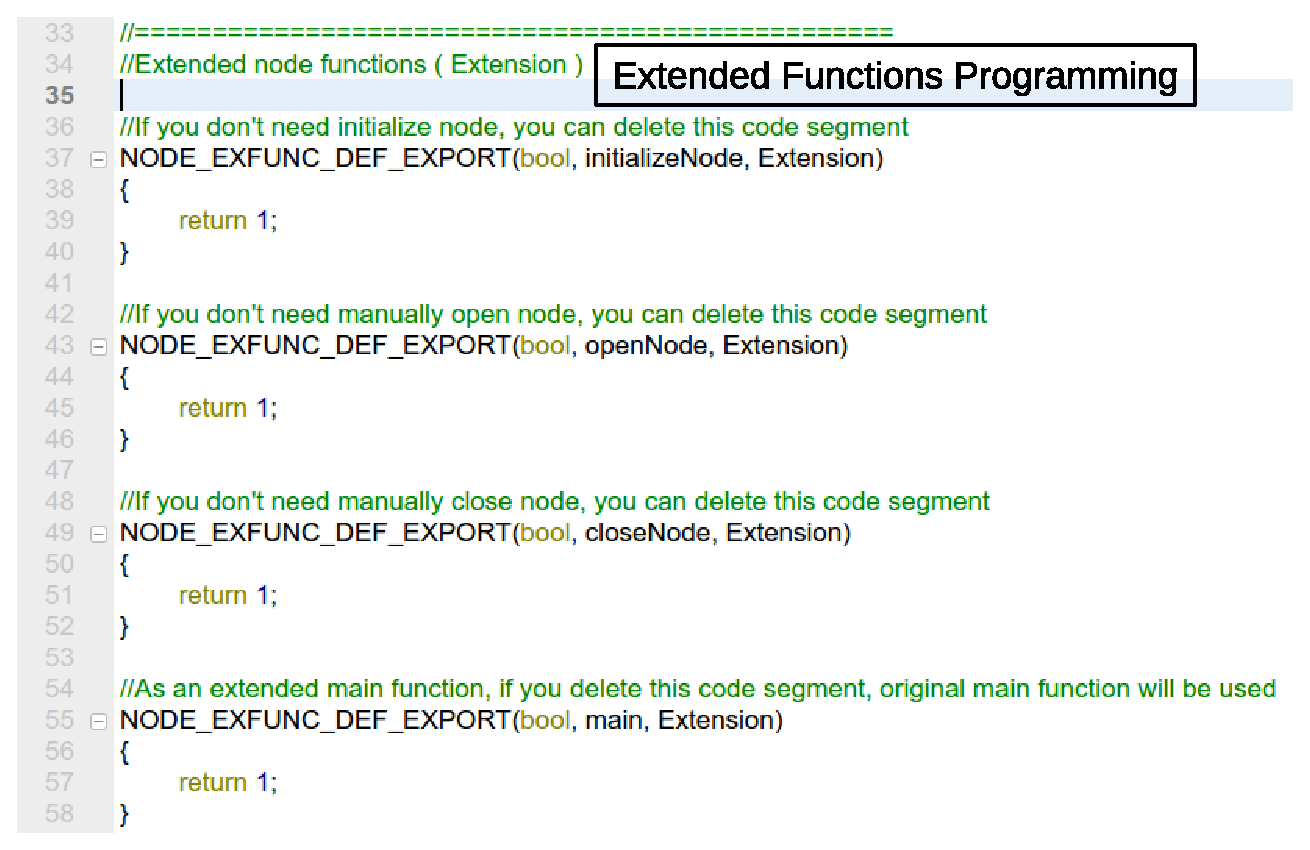
\includegraphics[width=0.6\textwidth]{img/source4.eps}
 \caption{Extended Functions}
 \label{fig:source4}
\end{figure}

\vspace{\fill}

\begin{framed}
 To develop a functional module, you only need to:
 \begin{itemize}
  \item remember the basic steps above
  \item use RobotSDK syntax below for programming
 \end{itemize}
 
 Now, we will show the most important part of this manual: RobotSDK Syntax. For convenience, we will start a new page here. We encourage users to print section \ref{syntax} out as handbook for functional module development. 
\end{framed}

\newpage

\section{RobotSDK Syntax}\label{syntax}

\subsection{Configure Node}

\begin{mdframed}
\begin{verbatim}
PORT_DECL(portID, inputNodeClass)
\end{verbatim}
\begin{itemize}
 \item Declare an input node with {\em{inputNodeClass}} for \#{\em{portID}} input port
 \item Arguments:
 \begin{itemize}
  \item portID: port id, must be a constant number
  \item inputNodeClass: "Node Class" of input node
 \end{itemize}
 \item Example:
 \begin{verbatim}
//=================================================
//Please add headers here:
#include"CameraSensor.h"
#include"VelodyneSensor.h"
#include<opencv2/opencv.hpp>
//=================================================
#include<RobotSDK.h>
//=================================================
//Node configuration

#undef NODE_CLASS
#define NODE_CLASS CameraVelodyneFusion

#undef INPUT_PORT_NUM
#define INPUT_PORT_NUM 2

#undef OUTPUT_PORT_NUM
#define OUTPUT_PORT_NUM 1

//Uncomment below PORT_DECL and set input node class name
PORT_DECL(0, CameraSensor)
PORT_DECL(1, VelodyneSensor)
 \end{verbatim}
 \item Note: \\~[Update-150427] The PORT\_DECL has been moved to cpp file for port toolkit.
\end{itemize}
\end{mdframed}

\subsection{Configure "Params", "Vars" and "Data"}

\subsubsection{"Params"}

\begin{mdframed}
\begin{verbatim}
NODE_PARAMS_TYPE
NODE_PARAMS_BASE_TYPE
\end{verbatim}
\begin{itemize}
 \item "Params" class name and "Params" base class name.
 \item Base class must be publicly inherited and "Params" can multi-inherit other class. 
\end{itemize}
\begin{itemize}
 \item Example:
 \begin{verbatim}
class NODE_PARAMS_TYPE : public NODE_PARAMS_BASE_TYPE
{

};
 \end{verbatim}
\end{itemize}
\end{mdframed}

\begin{mdframed}
\begin{verbatim}
NODE_PARAMS_TYPE_REF(RefNodeClassName)
\end{verbatim}
\begin{itemize}
 \item Refer to {\em{RefNodeClassName}}'s "Params" as its own "Params"
 \item Arguments:
 \begin{itemize}
  \item RefNodeClassName: "Node Class" of referred node.
 \end{itemize}
 \item Example:
 \begin{verbatim}
NODE_PARAMS_TYPE_REF(CameraSensor)
 \end{verbatim}
\end{itemize}
\end{mdframed}

\begin{mdframed}
\begin{verbatim}
INHERIT_NODE_PARAMS_TYPE(nodeClass)
\end{verbatim}
\begin{itemize}
 \item Inherite {/em{nodeClass}}'s "Params" type.
 \item Argument:
 \begin{itemize}
  \item nodeClass: node class of inherited node
 \end{itemize}
 \item Example:
 \begin{verbatim}
//VirtualScanGenerator Node
class NODE_PARAMS_TYPE : public NODE_PARAMS_BASE_TYPE
{
public:
    ADD_PARAM(uint, beamnum, 1000)
    ADD_PARAM(double, heightstep, 0.3)
    ADD_PARAM(double, slope, 30)
    ADD_PARAM(double, minfloor, -3)
    ADD_PARAM(double, maxceiling, 3)
    ADD_PARAM(double, maxfloor, -1.2)
    ADD_PARAM(double, minceiling, -0.5)
    ADD_PARAM(double, passheight, 2)
    ADD_PARAM(double, rotation, 3)
    ADD_PARAM(double, minrange, 0.5)
};

//VirtualScanCluster Node
class NODE_PARAMS_TYPE : INHERIT_NODE_PARAMS_TYPE(VirtualScanGenerator)
{
public:
    ADD_PARAM(uint, neighbornum, 5)
    ADD_PARAM(uint, minpointsnum, 10)
    ADD_PARAM(double, xsigma, 0.005)
    ADD_PARAM(double, xminsigma, 0.1)
    ADD_PARAM(double, ysigma, 0.05)
    ADD_PARAM(double, yminsigma, 0.1)
    ADD_PARAM(double, threshold, 0.08)
};
 \end{verbatim}
\end{itemize}
\end{mdframed}


\begin{mdframed}
\begin{verbatim}
ADD_PARAM(valueType, valueName, valueDefault)
ADD_ENUM_PARAM(valueType, valueName, valueDefault)
ADD_UENUM_PARAM(valueType, valueName, valueDefault)
\end{verbatim}
\begin{itemize}
 \item Add and register variable {\em{valueName}} in type {\em{valueType}} with default value {\em{valueDefault}}.
 \item The registered variable will be automatically managed by RobotSDK
 \item You can {\em{change}} its value via Robot-X Config Panel.
 \item Arguments:
 \begin{itemize}
  \item valueType: type of the variable
  \item valueName: name of the variable
  \item valueDefault: default value of the variable
 \end{itemize}
 \item Example:
 \begin{verbatim}
class NODE_PARAMS_TYPE : public NODE_PARAMS_BASE_TYPE
{
public:
    ADD_PARAM(QString, calibfilename, "#(CameraCalibFileName)")
};
 \end{verbatim}
 \item Note: \\It is not recommended to add an uninitialized variable in normal C++ way, because you cannot assign value to it in Node Function ("Params" is protected by const shared\_ptr).
\end{itemize}
\end{mdframed}

\begin{mdframed}
\begin{verbatim}
ADD_PARAM_WITH_OPTIONS(valueType, valueName, valueDefault, valueOptions)
ADD_ENUM_PARAM_WITH_OPTIONS(valueType, valueName, valueDefault, valueOptions)
ADD_UENUM_PARAM_WITH_OPTIONS(valueType, valueName, valueDefault, valueOptions)
\end{verbatim}
\begin{itemize}
 \item Add and register variable {\em{valueName}} in type {\em{valueType}} with default value {\em{valueDefault}} and options {\em{valueOptions}}.
 \item The registered variable will be automatically managed by RobotSDK
 \item You can {\em{choose}} its value via Robot-X Config Panel.
 \item Arguments:
 \begin{itemize}
  \item valueType: type of the variable
  \item valueName: name of the variable
  \item valueDefault: default value of the variable
  \item valueOptions: options of the variable
 \end{itemize}
 \item Example:
 \begin{verbatim}
class NODE_PARAMS_TYPE : public NODE_PARAMS_BASE_TYPE
{
public:
    ADD_PARAM_WITH_OPTIONS(double, angle, 0
                         , QList<double>()<<0<<90<<180<<270)
};
 \end{verbatim}
\end{itemize}
\end{mdframed}

\subsubsection{"Vars"}

\begin{mdframed}
\begin{verbatim}
NODE_VARS_TYPE
NODE_VARS_BASE_TYPE
\end{verbatim}
\begin{itemize}
 \item "Vars" class name and "Vars" base class name.
 \item Base class must be publicly inherited and "Vars" can multi-inherit other class. 
\end{itemize}
\begin{itemize}
 \item Example:
 \begin{verbatim}
class NODE_VARS_TYPE : public NODE_VARS_BASE_TYPE
{

};
 \end{verbatim}
\end{itemize}
\end{mdframed}

\begin{mdframed}
\begin{verbatim}
NODE_VARS_TYPE_REF(RefNodeClassName)
\end{verbatim}
\begin{itemize}
 \item Refer to {\em{RefNodeClassName}}'s "Vars" as its own "Vars"
 \item Arguments:
 \begin{itemize}
  \item RefNodeClassName: "Node Class" of referred node.
 \end{itemize}
 \item Example:
 \begin{verbatim}
NODE_VARS_TYPE_REF(ImageViewer)
 \end{verbatim}
\end{itemize}
\end{mdframed}

\begin{mdframed}
\begin{verbatim}
INHERIT_NODE_VARS_TYPE(nodeClass)
\end{verbatim}
\begin{itemize}
 \item Inherite {/em{nodeClass}}'s "Vars" type.
 \item Argument:
 \begin{itemize}
  \item nodeClass: node class of inherited node
 \end{itemize}
 \item Example:
 \begin{verbatim}
//ImageViewer Node
class NODE_VARS_TYPE : public NODE_VARS_BASE_TYPE
{
public:
    QVector<QRgb> colortable;
public:
    ADD_QLAYOUT(QHBoxLayout, layout)
    ADD_QWIDGET(QTabWidget, tabwidget)
    ADD_QWIDGET(QScrollArea, scrollarea)
    ADD_QWIDGET(QLabel, viewer, "Image Viewer")
};

//DPMModifier Node
class NODE_VARS_TYPE : INHERIT_NODE_VARS_TYPE(ImageViewer)
{
public:
    ADD_QWIDGET(DPMViewer, viewer)
public:
    ADD_INTERNAL_QWIDGET_TRIGGER(QPushButton, apply, "Output Change")
    ADD_INTERNAL_DEFAULT_CONNECTION(apply, clicked)
    ADD_QLAYOUT(QHBoxLayout, buttonlayout)
public:
      ADD_SYNC(dpmsync, 1)
};
 \end{verbatim}
\end{itemize}
\end{mdframed}

\begin{mdframed}
\begin{verbatim}
ADD_VAR(valueType, valueName, valueDefault)
ADD_ENUM_VAR(valueType, valueName, valueDefault)
ADD_UENUM_VAR(valueType, valueName, valueDefault)
\end{verbatim}
\begin{itemize}
 \item Add and register variable {\em{valueName}} in type {\em{valueType}} with default value {\em{valueDefault}}
 \item Arguments:
 \begin{itemize}
  \item valueType: type of the variable
  \item valueName: name of the variable
  \item valueDefault: default value of the variable
 \end{itemize}
 \item Example:
 \begin{verbatim}
class NODE_VARS_TYPE : public NODE_VARS_BASE_TYPE
{
public:
    cv::Mat extrinsicmat;
    cv::Mat cameramat;
    cv::Mat distcoeff;
public:
    ADD_VAR(QString, topic, "/image_raw")
    ADD_VAR(u_int32_t, queuesize, 1000)
    ADD_VAR(int, queryinterval, 10)
public:
    typedef ROSSub<sensor_msgs::ImageConstPtr> rossub;
    ADD_INTERNAL_QOBJECT_TRIGGER(rossub, camerasub, 1
                               , topic, queuesize, queryinterval)
    ADD_INTERNAL_DEFAULT_CONNECTION(camerasub, receiveMessageSignal)
};
 \end{verbatim}
 \item Note: \\It is recommended to add variable in non-standard type (no conversion between QString) in normal C++ way, because XML value manager does not know how to convert it. You can assign value to it in Node Function, because unlike "Params", "Vars" is not protected.
\end{itemize}
\end{mdframed}

\begin{mdframed}
\begin{verbatim}
ADD_VAR_WITH_OPTIONS(valueType, valueName, valueDefault, valueOptions)
ADD_ENUM_VAR_WITH_OPTIONS(valueType, valueName, valueDefault, valueOptions)
ADD_UENUM_VAR_WITH_OPTIONS(valueType, valueName, valueDefault, valueOptions)
\end{verbatim}
\begin{itemize}
 \item Add and register variable {\em{valueName}} in type {\em{valueType}} with default value {\em{valueDefault}} and options {\em{valueOptions}}.
 \item The registered variable will be automatically managed by RobotSDK
 \item You can {\em{choose}} its value via Robot-X Config Panel.
 \item Arguments:
 \begin{itemize}
  \item valueType: type of the variable
  \item valueName: name of the variable
  \item valueDefault: default value of the variable
  \item valueOptions: options of the variable
 \end{itemize}
 \item Example:
 \begin{verbatim}
class NODE_VARS_TYPE : public NODE_VARS_BASE_TYPE
{
public:
    ADD_VAR_WITH_OPTIONS(QString, topic, "/image_raw"
      , QList<QString>()<<"/image_raw"<<"/image_color"<<"/image_gray")
};
 \end{verbatim}
\end{itemize}
\end{mdframed}

\begin{mdframed}
\begin{verbatim}
ADD_INTERNAL_QOBJECT_TRIGGER(triggerType, triggerName, poolThreadFlag, ...)
\end{verbatim}
\begin{itemize}
 \item Add an internal QObject trigger {\em{triggerName}} in type {\em{triggerType}}.
 \item Arguments:
 \begin{itemize}
  \item triggerType: type of the internal trigger, must be derived from QObject
  \item triggerName: name of the internal trigger
  \item poolThreadFlag:
  \begin{itemize}
   \item =1, trigger will goto QObjectPoolThread and use inter-thread communication
   \item =0, trigger will stay with node and use intra-thread communication
  \end{itemize}
 
  \item ...: [Variadic arguments], used for arguments of trigger's construction function. 
 \end{itemize}
 \item Example:
 \begin{verbatim}
class NODE_VARS_TYPE : public NODE_VARS_BASE_TYPE
{
public:
    ADD_INTERNAL_QOBJECT_TRIGGER(QTimer, timer, 0)
    ADD_INTERNAL_DEFAULT_CONNECTION(timer, timeout)
};
 
class NODE_VARS_TYPE : public NODE_VARS_BASE_TYPE
{
public:
    cv::Mat extrinsicmat;
    cv::Mat cameramat;
    cv::Mat distcoeff;
public:
    ADD_VAR(QString, topic, "/image_raw")
    ADD_VAR(u_int32_t, queuesize, 1000)
    ADD_VAR(int, queryinterval, 10)
public:
    typedef ROSSub<sensor_msgs::ImageConstPtr> rossub;
    ADD_INTERNAL_QOBJECT_TRIGGER(rossub, camerasub, 1
                               , topic, queuesize, queryinterval)
    ADD_INTERNAL_DEFAULT_CONNECTION(camerasub, receiveMessageSignal)
};
 \end{verbatim}
\end{itemize}
\end{mdframed}

\begin{mdframed}
\begin{verbatim}
ADD_INTERNAL_QWIDGET_TRIGGER(triggerType, triggerName, ...)
\end{verbatim}
\begin{itemize}
 \item Add an internal QWidget trigger {\em{triggerName}} in type {\em{triggerType}}.
 \item QWidget trigger must stay in GUI thread (application thread)
 \item Arguments:
 \begin{itemize}
  \item triggerType: type of the internal trigger, must be derived from QObject
  \item triggerName: name of the internal trigger
  \item ...: [Variadic arguments], used for arguments of trigger's construction function. 
 \end{itemize}
 \item Example:
 \begin{verbatim}
class NODE_VARS_TYPE : public NODE_VARS_BASE_TYPE
{
public:
    ADD_INTERNAL_QWIDGET_TRIGGER(QPushButton, trigger, "Trigger")
    ADD_INTERNAL_DEFAULT_CONNECTION(trigger, clicked)
};
 \end{verbatim}
\end{itemize}
\end{mdframed}

\begin{mdframed}
\begin{verbatim}
ADD_INTERNAL_DEFAULT_CONNECTION(triggerName,signalName)
\end{verbatim}
\begin{itemize}
 \item Add an internal connection from {\em{triggerName}}'s signal {\em{signalName}} to node's slot "slotDefaultTrigger"
 \item "slotDefaultTrigger" of default node will call main Node Function and output "Data" if return value is true.
 \item "slotDefaultTrigger" is a virtual slot, user can re-implement it to change its behavior (node extension).
 \item Arguments:
 \begin{itemize}
  \item triggerName: name of the internal trigger
  \item signalName: name of the signal function
 \end{itemize}
 \item Example:
 \begin{verbatim}
class NODE_VARS_TYPE : public NODE_VARS_BASE_TYPE
{
public:
    cv::Mat extrinsicmat;
    cv::Mat cameramat;
    cv::Mat distcoeff;
public:
    ADD_VAR(QString, topic, "/image_raw")
    ADD_VAR(u_int32_t, queuesize, 1000)
    ADD_VAR(int, queryinterval, 10)
public:
    typedef ROSSub<sensor_msgs::ImageConstPtr> rossub;
    ADD_INTERNAL_QOBJECT_TRIGGER(rossub, camerasub, 1
                               , topic, queuesize, queryinterval)
    ADD_INTERNAL_DEFAULT_CONNECTION(camerasub, receiveMessageSignal)
};

class NODE_VARS_TYPE : public NODE_VARS_BASE_TYPE
{
public:
    ADD_INTERNAL_QWIDGET_TRIGGER(QPushButton, trigger, "Trigger")
    ADD_INTERNAL_DEFAULT_CONNECTION(trigger, clicked)
};
 \end{verbatim}
\end{itemize}
\end{mdframed}

\begin{mdframed}
\begin{verbatim}
ADD_INTERNAL_USER_CONNECTION(triggerName,signalName,slotName,...) 
\end{verbatim}
\begin{itemize}
 \item Add an internal connection from {\em{triggerName}}'s signal {\em{signalName}} to node's slot {\em{slotName}}
 \item You can use this to connect extended node's slot function.
 \item Arguments:
 \begin{itemize}
  \item triggerName: name of the internal trigger
  \item signalName: name of the signal function
  \item slotName: name of the slot function
  \item ...: [Variadic arguments], used for arguments' type of signal and slot functions. 
 \end{itemize}
 \item Example:
 \begin{verbatim}
class NODE_VARS_TYPE : public NODE_VARS_BASE_TYPE
{
public:
    ADD_INTERNAL_QWIDGET_TRIGGER(QCheckBox, checker, "Checker")
    ADD_INTERNAL_USER_CONNECTION(checker, stateChanged, slotExtended, int)
};
 \end{verbatim}
\end{itemize}
\end{mdframed}

\begin{mdframed}
\begin{verbatim}
ADD_QWIDGET(widgetType, widgetName, ...)
ADD_QLAYOUT(layoutType, layoutName, ...)
\end{verbatim}
\begin{itemize}
 \item Add QWidget or QLayout. They are not used as trigger.
 \item Arguments:
 \begin{itemize}
  \item widgetType: type of widget
  \item widgetName: name of widget
  \item layoutType: type of layout
  \item layoutName: name of layout
  \item ...: [Variadic arguments], used for arguments of widget's or layout's construction function. 
 \end{itemize}
 \item Example:
\begin{verbatim}
class NODE_VARS_TYPE : public NODE_VARS_BASE_TYPE
{
public:
    QVector<QRgb> colortable;
public:
    ADD_QLAYOUT(QHBoxLayout, layout)
    ADD_QWIDGET(QTabWidget, tabwidget)
    ADD_QWIDGET(QScrollArea, scrollarea)
    ADD_QWIDGET(QLabel, viewer, "Image Viewer")
};
\end{verbatim}
\end{itemize}
\end{mdframed}

\begin{mdframed}
\begin{verbatim}
ADD_CONNECTION(emitterName,signalName,receiverName,slotName,...)
\end{verbatim}
\begin{itemize}
 \item Add connection between {\em{emitterName}}'s signal {\em{signalName}} to {\em{receiverName}}'s slot {\em{slotName}}
 \item Arguments:
 \begin{itemize}
  \item emitterName: name of emitter, must be QObject or QWidget
  \item signalName: name of signal function
  \item receiverName: name of receiver, must be QObject or QWidget
  \item slotName: name of slot function
  \item ...: [Variadic arguments], used for arguments' type of signal and slot functions. 
 \end{itemize}
 \item Example:
\begin{verbatim}
class NODE_VARS_TYPE : public NODE_VARS_BASE_TYPE
{
public:
    ADD_INTERNAL_QOBJECT_TRIGGER(QTimer, timer, 0)
    ADD_INTERNAL_DEFAULT_CONNECTION(timer,timeout)
    ADD_QWIDGET(QPushButton, start, "Start")
    ADD_CONNECTION(start, clicked, timer, start)
    ADD_QWIDGET(QSpinBox, interval)
    ADD_CONNECTION(interval, valueChanged, timer, start, int)
};
\end{verbatim}
\end{itemize}
\end{mdframed}

\subsubsection{"Data"}

\begin{mdframed}
\begin{verbatim}
NODE_DATA_TYPE
NODE_DATA_BASE_TYPE
\end{verbatim}
\begin{itemize}
 \item "Data" class name and "Data" base class name.
 \item Base class must be publicly inherited and "Data" can multi-inherit other class. 
\end{itemize}
\begin{itemize}
 \item Example:
 \begin{verbatim}
class NODE_DATA_TYPE : public NODE_DATA_BASE_TYPE, public cv::Mat
{

};
 \end{verbatim}
\end{itemize}
\end{mdframed}

\begin{mdframed}
\begin{verbatim}
NODE_DATA_TYPE_REF(RefNodeClassName)
\end{verbatim}
\begin{itemize}
 \item Refer to {\em{RefNodeClassName}}'s "Data" as its own "Data"
 \item Arguments:
 \begin{itemize}
  \item RefNodeClassName: "Node Class" of referred node.
 \end{itemize}
 \item Example:
 \begin{verbatim}
NODE_DATA_TYPE_REF(VelodyneSensor)
 \end{verbatim}
\end{itemize}
\end{mdframed}

\begin{mdframed}
\begin{verbatim}
INHERIT_NODE_DATA_TYPE(nodeClass)
\end{verbatim}
\begin{itemize}
 \item Inherite {/em{nodeClass}}'s "Data" type.
 \item Argument:
 \begin{itemize}
  \item nodeClass: node class of inherited node
 \end{itemize}
 \item Example:
 \begin{verbatim}
//VirtualScanGenerator Node
class NODE_DATA_TYPE : public NODE_DATA_BASE_TYPE
{
public:
    cv::Mat extrinsicmat;
public:
    sensor_msgs::PointCloud2ConstPtr rospoints;
public:
    QVector<double> virtualscan;
    QVector<double> minheights;
    QVector<double> maxheights;
};

//VirtualScanCluster Node
class NODE_DATA_TYPE : INHERIT_NODE_DATA_TYPE(VirtualScanGenerator)
{
public:
    QVector<uint> labels;
    uint clusternum;
    QMultiMap<uint, uint> clusters;
};
 \end{verbatim}
\end{itemize}
\end{mdframed}

\subsection{Choose Node}

\begin{mdframed}
\begin{verbatim}
USE_DEFAULT_NODE
\end{verbatim}
\begin{itemize}
 \item Use default node
 \item Example:
\begin{verbatim}
#include"CameraSensor.h"

//If you need to use extended node, 
//please uncomment below and comment the using of default node
//USE_EXTENDED_NODE(ExtendedNodeClass[,...])
USE_DEFAULT_NODE
\end{verbatim}
\end{itemize}
\end{mdframed}

\begin{mdframed}
\begin{verbatim}
USE_EXTENDED_NODE(nodeType, ...)
\end{verbatim}
\begin{itemize}
 \item Use extended node as class {\em{nodeType}}
 \item Arguments:
 \begin{itemize}
  \item nodeType: class name of the extended node.
  \item ...: [Variadic arguments], used for arguments of extended node's construction function. 
 \end{itemize}
 \item Example:
\begin{verbatim}
#include"UDP.h"

//If you need to use extended node, 
//please uncomment below and comment the using of default node
USE_EXTENDED_NODE(SourceDrain)
//USE_DEFAULT_NODE
\end{verbatim}
\end{itemize}
\end{mdframed}

\subsection{Node Function}

\subsubsection{Node Function Declaration}

\begin{mdframed}
\begin{verbatim}
NODE_FUNC_DECL(returnType, funcName, ...)
NODE_EXFUNC_DECL(returnType, funcName, exName, ...)
\end{verbatim}
\begin{itemize}
 \item Declaration of Node Function and Extended Node Function
 \item Arguments:
 \begin{itemize}
  \item returnType: return type of Node Function
  \item funcName: name of Node Function
  \item exName: extended name of Node Function
  \item ...: [Variadic arguments], arguments of Node Function.
 \end{itemize}
 \item Example:
 \begin{verbatim}
NODE_FUNC_DECL(int, sum, int a, int b) // return a+b
NODE_EXFUNC_DECL(int, sum, squred, int a, int b) // return a^2+b^2
 \end{verbatim}
 \item Note: \\ The arguments of original Node Function and Extended ones should be same.
\end{itemize}
\end{mdframed}

\subsubsection{Node Function Definition}

\begin{mdframed}
\begin{verbatim}
NODE_FUNC_DEF_EXPORT(returnType, funcName, ...)
NODE_EXFUNC_DEF_EXPORT(returnType, funcName, exName, ...)
\end{verbatim}
\begin{itemize}
 \item Definition of Node Function and Extended Node Function
 \item Export with symbol, which can be resolved by QLibrary. Usually for interface functions.
 \item Arguments:
 \begin{itemize}
  \item returnType: return type of Node Function
  \item funcName: name of Node Function
  \item exName: extended name of Node Function
  \item ...: [Variadic arguments], arguments of Node Function.
 \end{itemize}
 \item Example:
 \begin{verbatim}
//This is original main function, you must keep it
NODE_FUNC_DEF_EXPORT(bool, main)
{
    return 1;
}
//If you don't need to initialize node, you can delete this code segment
NODE_EXFUNC_DEF_EXPORT(bool, initializeNode, Extension)
{
    return 1;
}
 \end{verbatim}
 \item Note: \\ The arguments of original Node Function and Extended ones should be same. \\ It does not need declaration in header.
\end{itemize}
\end{mdframed}

\begin{mdframed}
\begin{verbatim}
NODE_FUNC_DEF(returnType, funcName, ...)
NODE_EXFUNC_DEF(returnType, funcName, exName, ...)
\end{verbatim}
\begin{itemize}
 \item Definition of Node Function and Extended Node Function
 \item No symbol. QLibrary cannot resolve it. Usually for custom functions.
 \item Arguments:
 \begin{itemize}
  \item returnType: return type of Node Function
  \item funcName: name of Node Function
  \item exName: extended name of Node Function
  \item ...: [Variadic arguments], arguments of Node Function.
 \end{itemize}
 \item Example:
 \begin{verbatim}
NODE_FUNC_DEF(int, sum, int a, int b)
{
    return a+b;
}
NODE_EXFUNC_DEF(int, sum, squred, int a, int b)
{
    return a*a+b*b;
}
 \end{verbatim}
 \item Note: \\ The arguments of original Node Function and Extended ones should be same.
\end{itemize}
\end{mdframed}

\subsubsection{Access Node's Values}

\begin{mdframed}
\begin{verbatim}
NODE_PARAMS
NODE_VARS
NODE_DATA
\end{verbatim}
\begin{itemize}
 \item Access node's "Params", "Vars" and "Data" in Node Function
 \item Example:
\begin{verbatim}
NODE_FUNC_DEF_EXPORT(bool, main)
{
    auto params=NODE_PARAMS;
    auto vars=NODE_VARS;
    auto data=NODE_DATA;
    data->result=params->value+vars->LineEditWidget->text().toInt();
    return 1;
}
NODE_FUNC_DEF(int, sum, int a, int b)
{
    NODE_DATA->result=a+b+NODE_PARAMS->offset;
    return data->result;
}
\end{verbatim}
\item Note:\\ auto specifier is C++11 syntax (\url{http://en.cppreference.com/w/cpp/language/auto}). \\ "params", "vars" and "data" are variable name, you can use any others for instead.
\end{itemize}
\end{mdframed}

\subsubsection{Access Obtained Port's Values}

\begin{mdframed}
\begin{verbatim}
PORT_PARAMS_SIZE(portID)
PORT_DATA_SIZE(portID)
\end{verbatim}
\begin{itemize}
 \item The number of input "Params" and "Data" obtained from \#{\em{portID}} input port
 \item Arguments:
 \begin{itemize}
  \item portID: port id, must be a constant number.
 \end{itemize}
 \item Example:
 \begin{verbatim}
NODE_FUNC_DEF_EXPORT(bool, main)
{
    auto vars=NODE_VARS;
    int num=PORT_PARAMS_SIZE(0);
    vars->LabelWidget->setText(QString("Obtain %1 data").arg(num));
    return 1;
}
NODE_FUNC_DEF(int, sum)
{
    int i,num=PORT_DATA_SIZE(0);
    for(i=0;i<num;i++)
    {
        NODE_DATA->result+=PORT_DATA(0,i)->value;
    }
    return data->result;
}
 \end{verbatim}
\end{itemize}
\end{mdframed}

\begin{mdframed}
\begin{verbatim}
PORT_PARAMS(portID, paramsID)
PORT_DATA(portID, dataID)
\end{verbatim}
\begin{itemize}
 \item The {\em{paramsID}}-th input "Params" or {\em{dataID}}-th "Data" obtained from \#{\em{portID}} input port
 \item Small dataID $\Rightarrow$ new data; Large dataID $\Rightarrow$ old data.
 \item Arguments:
 \begin{itemize}
  \item portID: port id, must be a constant number.
  \item paramsID: params id in obtained params list.
  \item dataID: data id in obtained data list.
 \end{itemize}
 \item Example:
 \begin{verbatim}
NODE_FUNC_DEF_EXPORT(bool, main)
{
    int i,num=PORT_PARAMS_SIZE(0);
    for(i=0;i<num;i++)
    {
        auto inputparams=PORT_PARAMS(0,i);
        qDebug()<<QString("%1 from node %2::%3::%4")
            .arg(inputparams->_nodeclass)
            .arg(inputparams->_nodename)
            .arg(inputparams->_exname);
    }
    return 1;
}
NODE_FUNC_DEF(void, copyLatestTimeStamp)
{
    int num=PORT_DATA_SIZE(0);
    if(num>0)
    {
        NODE_DATA->timestamp=PORT_DATA(0,0)->timestamp;
    }
}
 \end{verbatim}
 \item Note: \\
 If there is only one input node for one port, input "Params" are same copy. \\
 If there are many input nodes for one port, copies of different nodes' "Params" are mixed. \\
 You can use its "\_nodeclass", "\_nodename" and "\_exname" to identify the source. \\
 NODE\_DATA\_TYPE inherits member "QTime timestamp" from NODE\_DATA\_BASE\_TYPE. \\
 You may get NULL pointer, therefore, it is better to check what you get.
\end{itemize}
\end{mdframed}

\begin{mdframed}
\begin{verbatim}
IS_INTERNAL_TRIGGER
\end{verbatim}
\begin{itemize}
 \item Judge the call is from data stream (input ports) or internal trigger.
 \item data stream call will pass valid port values.
 \item internal trigger call will pass invalid (empty) port values.
 \item Example:
\begin{verbatim}
//UDP Communication
NODE_FUNC_DEF_EXPORT(bool, main)
{
    auto vars=NODE_VARS;
    if(IS_INTERNAL_TRIGGER)
    {
        auto data=NODE_DATA;
        vars->udp->receiveData(data->message);
        return 1;
    }
    else
    {
        auto data=PORT_DATA(0,0);
        vars->udp->sendData(data->message);
        return 0;
    }
}
\end{verbatim}
\end{itemize}
\end{mdframed}

\subsubsection{Call Node Function}

\begin{mdframed}
\begin{verbatim}
NODE_FUNC(funcName, ...)
NODE_EXFUNC(funcName, exName, ...)
\end{verbatim}
\begin{itemize}
 \item Call Node Function from Node Function.
 \item Arguments:
 \begin{itemize}
  \item funcName: name of Node Function
  \item exName: extended name of Node Function
  \item ...: [Variadic arguments], arguments of Node Function.
 \end{itemize}
 \item Example:
 \begin{verbatim}
NODE_FUNC_DEF(int, sum, int a, int b)
{
    auto params=NODE_PARAMS;
    return a+b+params->offset;
}
NODE_FUNC_DEF_EXPORT(bool, main)
{
    auto vars=NODE_VARS;
    auto inputdata=PORT_DATA(0,0);
    auto data=NODE_DATA;
    data->result=NODE_FUNC(sum, inputdata->value, vars->value);   
    return 1;
}
 \end{verbatim}
\end{itemize}
\end{mdframed}

\subsection{Obtain Values from Input Ports}

\subsubsection{Obtain Behavior}

\begin{mdframed}
\begin{verbatim}
enum ObtainBehavior
{
    CopyOldest=NUM_0,
    GrabOldest=NUM_1,
    CopyLatest=NUM_2,
    GrabLatest=NUM_3,
    CopyOldestStrictly=NUM_4,
    GrabOldestStrictly=NUM_5,
    CopyLatestStrictly=NUM_6,
    GrabLatestStrictly=NUM_7
};
\end{verbatim}
\begin{itemize}
 \item Explanation:
 \begin{itemize}
  \item CopyOldest: Copy the oldest "Params" and "Data" without removing.
  \item GrabOldest: Grab the oldest "Params" and "Data" with removing.
  \item CopyLatest: Copy the latest "Params" and "Data" without removing.
  \item GrabLatest: Grab the latest "Params" and "Data" with clearing buffer.
  \item CopyOldestStrictly: If the all input buffer count fulfill requirement, CopyOldest.
  \item GrabOldestStrictly: If the all input buffer count fulfill requirement, GrabOldest.
  \item CopyLatestStrictly: If the all input buffer count fulfill requirement, CopyLatest.
  \item GrabLatestStrictly: If the all input buffer count fulfill requirement, GrabLatest.
  \end{itemize}
  \item Set it via NODE\_VARS's functions in any Node Functions any time.
\begin{verbatim}
void setInputPortObtainDataBehavior(uint portID
                              , ObtainBehavior obtainDataBehavior);
void setInputPortObtainDataBehavior(QList<ObtainBehavior> obtainDataBehavior);
\end{verbatim}
  \item Example:
\begin{verbatim}
NODE_FUNC_DEF_EXPORT(bool, initializeNode)
{
    auto vars=NODE_VARS;
    vars->setInputPortObtainDataBehavior(0, CopyOldest);
    vars->setInputPortObtainDataBehavior(QList< ObtainBehavior >()
              <<CopyOldest<<GrabOldest);
    return 1;
}
\end{verbatim}
 \item Note: \\ Default value is "GrabLatest" \\ It is safe when portID is out of range or list size does not equal input port size
\end{itemize}
\end{mdframed}


\subsubsection{Obtain Parameters}

\begin{mdframed}
\begin{itemize}
 \item Parameters List (all in NODE\_VARS):
 \begin{itemize}
  \item buffersize: maximum input buffer size
  \begin{itemize}
   \item 0: without size limitation.
   \item $>$0: with size limitation.
   \item Default: 0
   \item Functions:
   \begin{verbatim}
void setInputPortBufferSize(uint portID, uint bufferSize);
void setInputPortBufferSize(QList< uint > bufferSize);
   \end{verbatim}
  \end{itemize}
  \item obtaindatasize: size of obtain values each time
  \begin{itemize}
   \item 0: obtain all values in the buffer.
   \item $>$0: obtain certain size of values. Threshold for "Strictly" obtain behavior.
   \item Default: 1
   \item Functions:
   \begin{verbatim}
void setInputPortObtainDataSize(uint portID, uint obtainDataSize);
void setInputPortObtainDataSize(QList< uint > obtainDataSize);
   \end{verbatim}
  \end{itemize}
  \item triggerflag: flag to allow port to trigger node
  \begin{itemize}
   \item false: not allowed.
   \item true: allowed.
   \item Default: true
   \item Functions:
      \begin{verbatim}
void setInputPortTriggerFlag(uint portID, bool triggerFlag);
void setInputPortTriggerFlag(QList< bool > triggerFlag);
   \end{verbatim}
  \end{itemize}
  \item Example:
  \begin{verbatim}
NODE_FUNC_DEF_EXPORT(bool, initializeNode)
{
    auto vars=NODE_VARS;
    
    vars->setInputPortObtainDataBehavior(0, GrabOldestStrictly);
    vars->setInputPortBufferSize(0, 10);
    vars->setInputPortObtainDataSize(0, 10);

    vars->setInputPortBufferSize(1, 0);
    vars->setInputPortObtainDataSize(1, 0);
    
    vars->setInputPortTriggerFlag(QList<bool>()<<1<<0);
    return 1;
}
\end{verbatim}
 \end{itemize}
 \item Note: \\ You can set them in any Node Functions any time. \\It is safe when portID is out of range or list size does not equal input port size
\end{itemize}
\end{mdframed}

\subsection{Emit Values from Output Ports}

\begin{mdframed}
\begin{itemize}
 \item Parameters List (in NODE\_DATA):
 \begin{itemize}
  \item filterflag: flag to filter output ports
  \begin{itemize}
   \item false: Values will not be emitted from this port.
   \item true or NULL: Values will be emitted from this port.
   \item Default: NULL
   \item Functions:
   \begin{verbatim}
void setOutputPortFilterFlag(QList< bool > filterFlag);
   \end{verbatim}
  \end{itemize}
  \item Example:
  \begin{verbatim}
NODE_FUNC_DEF_EXPORT(bool, main)
{
    auto data=NODE_DATA;
    uint out=qrand()%2;
    if(out==0)
    {
        data->setOutputPortFilterFlag(QList<bool>()<<0<<1);
    }
    else
    {
        data->setOutputPortFilterFlag(QList<bool>()<<1<<0);
    }
    return 1;
}
\end{verbatim}
 \end{itemize}
 \item Note: \\ You can set it in any Node Functions except for "initializeNode", "openNode" and "closeNode" any time. \\It is safe when list size does not equal input port size \\ If not set, all ports are allowed to emit values.
\end{itemize}
\end{mdframed}

\subsection{Node's Flags}

\subsubsection{GUI Thread Flag}

\begin{mdframed}
\begin{itemize}
 \item Parameters List (in NODE\_VARS):
 \begin{itemize}
  \item guithreadflag: flag to move node into GUI thread.
  \begin{itemize}
   \item false: Node will go to its own thread.
   \item true: Node will stay in GUI thread.
   \item Default: false
   \item Functions:
   \begin{verbatim}
void setNodeGUIThreadFlag(bool guiThreadFlag);
   \end{verbatim}
  \end{itemize}
  \item Example:
  \begin{verbatim}
NODE_FUNC_DEF_EXPORT(bool, initializeNode)
{
    auto vars=NODE_VARS;
    vars->setNodeGUIThreadFlag(1);
    return 1;
}
\end{verbatim}
 \end{itemize}
 \item Note: \\ You can only set it in "initializeNode" Node Function. \\ If node wants to control (write operation) its widgets, this must be set to false.
\end{itemize}
\end{mdframed}

\subsubsection{Show Widget Flag}

\begin{mdframed}
\begin{itemize}
 \item Parameters List (in NODE\_VARS):
 \begin{itemize}
  \item showwidgetflag: flag to allow non-GUI node to show widget.
  \begin{itemize}
   \item false: Non-GUI node is not allowed to show widget.
   \item true: Non-GUI node is allowed to show widget.
   \item Default: false
   \item Functions:
   \begin{verbatim}
void setNodeShowWidgetFlag(bool showWidgetFlag);
   \end{verbatim}
  \end{itemize}
  \item Example:
  \begin{verbatim}
NODE_FUNC_DEF_EXPORT(bool, initializeNode)
{
    auto vars=NODE_VARS;
    vars->setNodeShowWidgetFlag(1);
    return 1;
}
\end{verbatim}
 \end{itemize}
 \item Note: \\ You can set it in any Node Functions any time. \\ It only affects non-GUI node. \\ If non-GUI node only reads its widgets or is triggered by its widgets, this could be set to true.
\end{itemize}
\end{mdframed}

\subsection{Node Central Widget}

\begin{mdframed}
\begin{itemize}
 \item Every node has its own central widget stored in NODE\_VARS and named as "widget".
 \item All widgets in NODE\_VARS should embed into "widget", which could be shown by Robot-X.
 \item Its default state is invisible and is controlled by guithreadflag and showwidgetflag.
 \item Example:
 \begin{verbatim}
NODE_FUNC_DEF_EXPORT(bool, initializeNode)
{
    auto vars=NODE_VARS;
    vars->viewer->setAlignment(Qt::AlignCenter); //QLabel
    vars->scrollarea->setWidget(vars->viewer); //QScrollArea
    vars->tabwidget->addTab(vars->scrollarea,"TimeStamp"); //QTabWidget
    vars->layout->addWidget(vars->tabwidget); //QHBoxLayout
    vars->widget->setLayout(vars->layout); //central widget
    vars->setNodeGUIThreadFlag(1);
    return 1;
}
 \end{verbatim}

\end{itemize}

\end{mdframed}

\subsection{Sync}

\begin{mdframed}
\begin{verbatim}
ADD_SYNC(syncName, basePortID)
\end{verbatim}
\begin{itemize}
 \item This should be used in "Vars" and it will add a Sync to "Vars"
 \item Arguments:
 \begin{itemize}
  \item syncName: name of Sync
  \item basePortID: indicates which port is the base for Sync (extract one by one)
 \end{itemize}
 \item Example:
\begin{verbatim}
//=================================================
//Node configuration

#undef NODE_CLASS
#define NODE_CLASS DPMModifier

#undef INPUT_PORT_NUM
#define INPUT_PORT_NUM 2

#undef OUTPUT_PORT_NUM
#define OUTPUT_PORT_NUM 1

//Uncomment below PORT_DECL and set input node class name
PORT_DECL(0, CameraSensor)
PORT_DECL(1, DPMDetector)

//=================================================
/*...*/
class NODE_VARS_TYPE : public NODE_VARS_BASE_TYPE
{
public:
      ADD_SYNC(dpmsync, 1)
};
\end{verbatim}
\item  Node: \\ You can add as many as Syncs simutaneously.
\end{itemize}
\end{mdframed}

\begin{mdframed}
\begin{verbatim}
SYNC_START(sync)
\end{verbatim}
\begin{itemize}
 \item If you have a Sync, you need to call SYNC\_START at least for one time during "Excecution" loop.
 \item Argument:
 \begin{itemize}
  \item sync: Sync instance
 \end{itemize}
 \item Example:
\begin{verbatim}
NODE_FUNC_DEF_EXPORT(bool, main)
{
    auto vars=NODE_VARS;
    bool flag=SYNC_START(vars->dpmsync);
    if(flag)
    {
        auto imagedata=SYNC_DATA(vars->dpmsync,0);
        auto dpmdata=SYNC_DATA(vars->dpmsync,1);
        /*...*/
    }
    return 1;
}
\end{verbatim}
\item Node: \\
This call will return a boolean flag to indicate whether the Sync has available synchronized data. \\
If the Sync has synchronized data, then the synchronized data will be moved to ready-to-read array from synchronizing buffer.
\end{itemize}
\end{mdframed}

\begin{mdframed}
\begin{verbatim}
SYNC_PARAMS(sync, portID)
SYNC_DATA(sync, portID)
\end{verbatim}
\begin{itemize}
 \item Get Synchronized input "Params" and "Data" from Sync's ready-to-read array
 \item Example:
 \begin{itemize}
  \item sync: Sync instance
  \item portID: port id of desired input "Params" and "Data", must be constant number.
 \end{itemize}
 \item Example:
\begin{verbatim}
NODE_FUNC_DEF_EXPORT(bool, main)
{
    auto vars=NODE_VARS;
    while(SYNC_START(vars->dpmsync))
    {
        auto imagedata=SYNC_DATA(vars->dpmsync,0);
        auto dpmdata=SYNC_DATA(vars->dpmsync,1);
        /*...*/
    }
    return 1;
}
\end{verbatim}
\item Note: \\ It will get same value unless you call SYNC\_START again.
\end{itemize}
\end{mdframed}


\chapter{Node Extension: Customize Node Behavior} \label{nodeextension}

Node extension is an advanced topic and it is not neccessary for common top-down modular software development. Therefore, in this chapter, we will briefly introduce how to extend default node.

\section{Extend Default Node}

\subsection{Default Node}

As shown in Fig.\ref{fig:defaultnode}, the default node behavior contains two routes to access "Main Entry" (main Node Function in module) and then emit its "Params" and new "Data" according to the boolean return value of "Main Entry". The first route starts from "Input Ports" and node's virtual slot function "slotObtainParamsData" is called (inter-thread call). This route passes input "Params" and "Data" to the "Main Entry". The second route starts from "Internal Triggers" and node's virtual slot function "slotDefaultTrigger" is called (inter-thread call if the trigger is in "QObjectPoolThread" or is a QWidget, otherwise intra-thread call). This route does not pass input "Params" and "Data" to the "Main Entry".

\begin{figure}
\centering
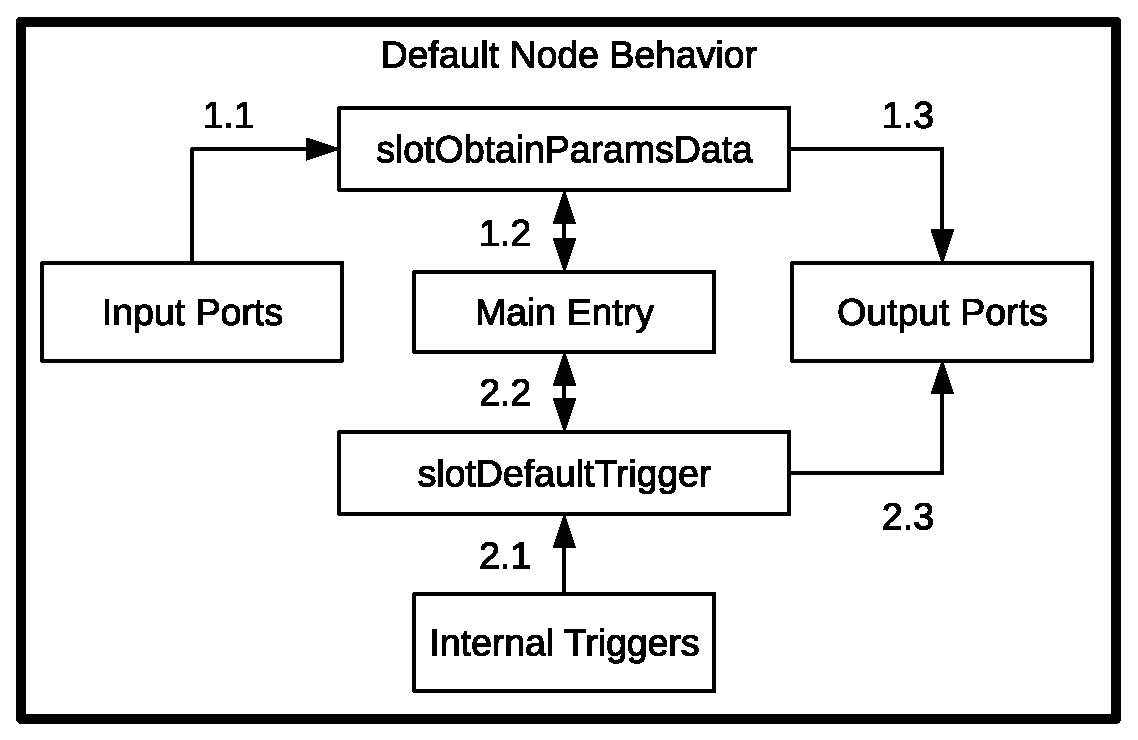
\includegraphics[width=0.6\textwidth]{img/defaultnode.eps}
\caption{Default Node Behavior}
\label{fig:defaultnode}
\end{figure}

\subsection{5 Kinds of Extension}

Developers can extend default node's behavior by inheriting default "Node" class and there are 5 things you can do for extension.

\begin{enumerate}
 \item Re-implement virtual slot function "slotObtainParamsData" to modify "1.2" and "1.3" in Fig.\ref{fig:defaultnode}.
 \item Re-implement virtual slot function "slotDefaultTrigger" to modify "2.2" and "2.3" in Fig.\ref{fig:defaultnode}.
 \item Add new slot functions to enrich "2.1" ends in Fig.\ref{fig:defaultnode}.
 \item Add new interface functions for new entries.
 \item Add new signal functions for high-level application development\\ (original Robot-X couldn't work with new signal functions, but you can extend it with slot functions).
\end{enumerate}

The source code files of extended node class could be put anywhere, for example, in the module project, in the Kernel or standalone as compiled static library. Below we will show some examples about these 5 kinds of extension without too much details.

\subsubsection{1st Extension}

\begin{mdframed}
\begin{itemize}
 \item Original "slotObtainParamsData"
 \begin{verbatim}
void Node::slotObtainParamsData(PORT_PARAMS_CAPSULE inputParams
                              , PORT_DATA_CAPSULE inputData)
{
    INPUT_PARAMS_ARG=inputParams;
    INPUT_DATA_ARG=inputData;
    NODE_DATA_ARG=generateNodeData();
    if(NODE_FUNC_PTR(main))
    {
        emit signalSendParamsData(NODE_PARAMS_ARG,NODE_DATA_ARG);
    }
}
 \end{verbatim}
\item Extension Example:\\
Assume we have defined another entry as "ExMain" with "int" type return value and additional argument QTime (see "4th Extension"), and we also add a signal function "signalExecutionResult(int returnValue)" (see "5th Extension"). We can extend "slotObtainParamsData" as:
\begin{verbatim}
//header
#include<node.h>
namespace RobotSDK
{
class ExNode : public Node
{
public slots:
    void slotObtainParamsData(PORT_PARAMS_CAPSULE inputParams
                            , PORT_DATA_CAPSULE inputData);
    /*...*/
}
}

//source
using namespace RobotSDK;
void ExNode::slotObtainParamsData(PORT_PARAMS_CAPSULE inputParams
                                , PORT_DATA_CAPSULE inputData)
{
    INPUT_PARAMS_ARG=inputParams;
    INPUT_DATA_ARG=inputData;
    NODE_DATA_ARG=generateNodeData();
    QTime time=QTime::currentTime();
    int result=NODE_FUNC_PTR(ExMain, time);
    emit signalExecutionResult(result);
}
}

//module source
USE_EXTENDED_NODE(ExNode)
\end{verbatim}
\end{itemize}
\end{mdframed}

\subsubsection{2nd Extension}

\begin{mdframed}
 \begin{itemize}
  \item Original "slotDefaultTrigger"
  \begin{verbatim}
void Node::slotDefaultTrigger()
{
    INPUT_PARAMS_ARG.clear();
    INPUT_DATA_ARG.clear();
    NODE_DATA_ARG=generateNodeData();
    if(NODE_FUNC_PTR(main))
    {
        emit signalSendParamsData(NODE_PARAMS_ARG,NODE_DATA_ARG);
    }
}
  \end{verbatim}
 \end{itemize}
 \item Extension Example:\\ With same assumption of "1st Extension"
\begin{verbatim}
//header
#include<node.h>
namespace RobotSDK
{
class ExNode : public Node
{
public slots:
    void slotDefaultTrigger();
    /*...*/
}
}

//source
using namespace RobotSDK;
void ExNode::slotDefaultTrigger()
{
    INPUT_PARAMS_ARG.clear();
    INPUT_DATA_ARG.clear();
    NODE_DATA_ARG=generateNodeData();
    QTime time=QTime::currentTime();
    int result=NODE_FUNC_PTR(ExMain, time);
    emit signalExecutionResult(result);
    if(result>0)
    {
        emit signalSendParamsData(NODE_PARAMS_ARG,NODE_DATA_ARG);
    }
}

//module source
USE_EXTENDED_NODE(ExNode)
\end{verbatim}
\end{mdframed}

\subsubsection{3rd Extension}

\begin{mdframed}
\begin{itemize}
 \item Extension Example: \\ With same assumption of "1st Extension"
\begin{verbatim}
//header
#include<node.h>
namespace RobotSDK
{
class ExNode : public Node
{
public slots:
    void slotExtendedTrigger(int msecs);
    /*...*/
}
}

//source
using namespace RobotSDK;
void ExNode::slotExtendedTrigger(int msecs)
{
    INPUT_PARAMS_ARG.clear();
    INPUT_DATA_ARG.clear();
    NODE_DATA_ARG=generateNodeData();
    QTime time=QTime::fromMSecsSinceStartOfDay(msecs);
    int result=NODE_FUNC_PTR(ExMain, time);
    emit signalExecutionResult(result);
}

//module header
class NODE_VARS_TYPE : public NODE_VARS_BASE_TYPE
{
public:
    ADD_INTERNAL_QWIDGET_TRIGGER(QSpinBox, timeMsec, 0)
    ADD_QWIDGET(QSpinBox, interval)
    ADD_INTERNAL_USER_CONNECTION(QSpinBox, valueChanged
                               , slotExtendedTrigger, int)
};

//module source
USE_EXTENDED_NODE(ExNode)
\end{verbatim}
\end{itemize}
\end{mdframed}

\subsubsection{4th Extension}

\begin{mdframed}
\begin{itemize}
 \item Extension Example: \\ Realize assumptions used above
\begin{verbatim}
//header
#include<node.h>
namespace RobotSDK
{
class ExNode : public Node
{
public:
    ADD_NODE_FUNC_PTR(int, ExMain, 1, QTime time)
    /*...*/
}
}

//module source
USE_EXTENDED_NODE(ExNode)

NODE_FUNC_DEF_EXPORT(int, ExMain, QTime time)
{
    auto data=NODE_DATA;
    data->second=time.second();
    return data->second;
}
\end{verbatim}
\end{itemize}
\end{mdframed}

\subsubsection{5th Extension}

\begin{mdframed}
\begin{itemize}
 \item Extension Example: \\ Realize assumptions used above
\begin{verbatim}
//header
#include<node.h>
namespace RobotSDK
{
class ExNode : public Node
{
signals:
    void signalExecutionResult(int result);
    /*...*/
}
}

//Extension of Robot-X (code segments)
#include<exnode.h> //[Extension]
/*...*/
RobotSDK::Graph * graph=new RobotSDK::Graph; //[Robot-X]
/*...*/
QString nodeFullName, libraryFileName, configFileName; //[Robot-X]
/*...*/
graph->addNode(nodeFullName, libraryFileName, configFileName); //[Robot-X]
/*...*/
//[Extension]
RobotSDK::Node * node=graph->getNode(nodeFullName);
connect(node, SIGNAL(signalExecutionResult(int))
      , this, SLOT(slotExecutionResult(int)));
/*...*/
\end{verbatim}
\end{itemize}
\end{mdframed}

\section{RobotSDK Syntax for Node Extension}

\begin{mdframed}
\begin{verbatim}
ADD_NODE_FUNC_PTR(returnType, funcName, mandatoryFlag, ...)
\end{verbatim}
\begin{itemize}
 \item Add an interface function to link module's Node Function.
 \item It will be automatically managed by RobotSDK.
 \item Arguments:
 \begin{itemize}
  \item returnType: return type of interface function.
  \item funcName: name of interface function
  \item mandatoryFlag: flag to show whether it is a mandatory interface function
  \begin{itemize}
   \item false: RobotSDK will try to link it to module, if failed, node will still be constructed.
   \item true: RobotSDK will try to link it to module, if failed, node will not be constructed.
  \end{itemize}
  \item ...: [Variadic arguments], used for arguments of interface function. 
 \end{itemize}
 \item Example: \\ see "4th Extension"
\end{itemize}
\end{mdframed}

\begin{mdframed}
\begin{verbatim}
NODE_FUNC_PTR(funcName, ...)
\end{verbatim}
\begin{itemize}
 \item Load an interface function.
 \item Arguments:
 \begin{itemize}
  \item funcName: name of interface function
  \item ...: [Variadic arguments], used for arguments of interface function. 
 \end{itemize}
 \item Example: \\ see "1st, 2nd and 3rd Extenstions"
\end{itemize}
\end{mdframed}

\begin{mdframed}
\begin{verbatim}
CHECK_NODE_FUNC_PTR(funcName)
\end{verbatim}
\begin{itemize}
 \item Check whether an interface function is available if it is not mandatory.
 \item Arguments:
 \begin{itemize}
  \item funcName: name of interface function
 \end{itemize}
 \item Example: 
\begin{verbatim}
//in Kernel header
class Node : public QObject
{
    /*...*/
    ADD_NODE_FUNC_PTR(bool, openNode, 0)
    /*...*/
}

//in Kernel source (code segment)
if(CHECK_NODE_FUNC_PTR(openNode))
{
    _openflag=NODE_FUNC_PTR(openNode);
}
\end{verbatim}
\end{itemize}
\end{mdframed}

\end{document}
